\documentclass{dissertation}

\begin{document}

%% Specify the title and author of the thesis. This information will be used on
%% the title page (in title/title.tex) and in the metadata of the final PDF.
\title[Algorithm to estimate the minimal time path for Laser Sailing ]{Effects of time steps on the opimal path}
\author{Gabriela}{Pardo Arteaga}

%% Use Roman numerals for the page numbers of the title pages and table of
%% contents.
\frontmatter

\begin{titlepage}

\begin{center}

%% Extra whitespace at the top.
\vspace*{2\bigskipamount}

%% Print the title.
{\makeatletter
\titlestyle\bfseries\LARGE\@title
\makeatother}

%% Print the optional subtitle.
{\makeatletter
\ifx\@subtitle\undefined\else
    \bigskip
    \titlefont\titleshape\Large\@subtitle
\fi
\makeatother}

\end{center}

\cleardoublepage
\thispagestyle{empty}

\begin{center}

%% The following lines repeat the previous page exactly.

\vspace*{2\bigskipamount}

%% Print the title.
{\makeatletter
\titlestyle\bfseries\LARGE\@title
\makeatother}

%% Print the optional subtitle.
{\makeatletter
\ifx\@subtitle\undefined\else
    \bigskip
    \titlefont\titleshape\Large\@subtitle
\fi
\makeatother}

%% Uncomment the following lines to insert a vertically centered picture into
%% the title page.
%\vfill
%\includegraphics{title}
\vfill

%% Apart from the names and dates, the following text is dictated by the
%% promotieregelement.

{\Large\titlefont\bfseries Proefschrift}

\bigskip
\bigskip

ter verkrijging van de graad van doctor

aan de Technische Universiteit Delft,

op gezag van de Rector Magnificus prof.~ir.~K.C.A.M.~Luyben,

voorzitter van het College voor Promoties,

in het openbaar te verdedigen op dinsdag 1 januari 2015 om 10:00 uur

\bigskip
\bigskip

door

\bigskip
\bigskip

%% Print the full name of the author.
\makeatletter
{\Large\titlefont\bfseries\@firstname\ {\titleshape\@lastname}}
\makeatother

\bigskip
\bigskip

Fachlehrer für Mathematik und Physik, \\
Eidgenössische Polytechnische Schule, Zürich, Zwitserland,

geboren te Ulm, Duitsland.

%% Extra whitespace at the bottom.
\vspace*{2\bigskipamount}

\end{center}

\clearpage
\thispagestyle{empty}

%% The following line is dictated by the promotieregelement.
\noindent Dit proefschrift is goedgekeurd door de

%% List the promotors (supervisors).
\medskip\noindent
\begin{tabular}{l}
    promotor: prof.\ dr.\ A.\ Kleiner \\
    copromotor: dr.\ A.A.\ Aaronson
\end{tabular}

\bigskip
\noindent Samenstelling promotiecommissie:

%% List the committee members, starting with the Rector Magnificus and the
%% promotor(s) and ending with the reserve members.
\medskip\noindent
\begin{tabular}{p{3cm}l}
    Rector Magnificus, & voorzitter \\
    Prof.\ dr.\ A.\ Kleiner, & Technische Universiteit Delft \\
    Dr.\ A.A.\ Aaronson, & Technische Universiteit Delft \\

    \medskip
    \mbox{\emph{Onafhankelijke leden:}} & \\

    Prof.\ dr.\ A.\ Jansen & Technische Universiteit Delft \\
    % Special case, only for very long names
    \mbox{Prof.\ dr.\ ir.\ A.B.C.D.\ van de Lange-Achternaam} & \\
      & Technische Universiteit Delft \\
    Prof.\.dr.\ N.\ Nescio & Politecnico di Milano, Itali\"e \\
    Prof.\ dr.\ ir.\ J.\ Doe, & Technische Universiteit Delft, reservelid \\

    \medskip
    \mbox{\emph{Overige leden:}} & \\
    Prof.\ dr.\ ir.\ J.\ de Wit, & Technische Universiteit Delft \\
    Dr.\ ir.\ Q.\ de Zwart, & Technische Universiteit Eindhoven \\
\end{tabular}

%% Include the following disclaimer for committee members who have contributed
%% to this dissertation. Its formulation is again dictated by the
%% promotieregelement.
\medskip
\noindent Prof.\ dr.\ ir.\ J.\ de Wit heeft in belangrijke mate aan de totstandkoming van het proefschrift bijgedragen.

%% Here you can include the logos of any institute that contributed financially
%% to this dissertation.
\vfill
\begin{center}
    
\includegraphics[height=0.5in]{title/logos/tudelft}
    \hspace{2em}
    
\includegraphics[height=0.5in]{title/logos/casimir} \\
    
\includegraphics[height=0.5in]{title/logos/fom}
    \hspace{2em}
    
\includegraphics[height=0.5in]{title/logos/nwo}
\end{center}
\vfill

\noindent
\begin{tabular}{@{}p{0.2\textwidth}@{}p{0.8\textwidth}}
    \textit{Keywords:} & \ldots \\[\medskipamount]
    \textit{Printed by:} & Johannes Gutenberg \\[\medskipamount]
    \textit{Front \& Back:} & Beautiful cover art that captures the entire content of this thesis in a single illustration.
\end{tabular}

\vspace{4\bigskipamount}

\noindent Copyright \textcopyright\ 2015 by A.~Einstein

%% Uncomment the following lines if this dissertation is part of the Casimir PhD
%% Series, or a similar research school.
%\medskip
%\noindent Casimir PhD Series, Delft-Leiden 2015-01

\medskip
\noindent ISBN 000-00-0000-000-0

\medskip
\noindent An electronic version of this dissertation is available at \\
\url{http://repository.tudelft.nl/}.

\end{titlepage}



%% The (optional) dedication can be used to thank someone or display a
%% significant quotation.
\dedication{\epigraph{Curiosity is the starling unexpectedness \\ of all beginnings.}{Hannah Arendt}}

\tableofcontents

%%%Summary Abstract
\chapter*{Summary}
\addcontentsline{toc}{chapter}{Summary}
\setheader{Summary}

%Integrating new technologies on training programs for professional athletes have been increases in the last years. Olympic sailing uses the approach of one-boat design hence improvements on the boat are not allowed. Because of this, the scope for many  types of research is on enhancing the strength and other motor skills of athletes rather than strategy methods to help them train. As in many race competitions, the winner is the one that first crosses the end line. Olympic sailing regattas stand for different days and races with distinct configurations for the route and weather conditions. This means the winner had crossed the line not only one time but in most of the races.\par \noindent
%In addition, athletes are not allowed to get any information or feedback from coaches during the race, in consequence, the information of how to course the race is crucial not only for the race but also for its preparation and training. To win, the athletes confront the weather variations and its uncertainty taking different decisions. One of these decisions refers to the sailing direction taken at any start line, the other decision that impacts the results is the number of maneuvers when the boat sails against the wind. \par  % that can be started on the left or right hand side.  , known as a zig-zag pattern

This study develops an algorithm on \acrshort{matlab} to model the path for sailing competitions and optimize the minimal time shaped by a wind of sailing races for the Laser (Olympic class). Furthermore, to identify the effects of time-steps of different size on the resulting times and trajectories. For the validation of the algorithm, this research compares the results between the algorithm using alternative scenarios and the results from the race. One of these scenarios uses the wind measured during the race. The reference race is R1 from the World Cup Series 2018 at Hyères, France. \par  

%Integrating new technologies on training programs for professional athletes have been increases in the last years. Olympic sailing uses the approach of one-boat design hence improvements on the boat are not allowed. Because of this, the scope for many  types of research is on enhancing the strength and other motor skills of athletes rather than strategy methods to help them train. As in many race competitions, the winner is the one that first crosses the end line. Olympic sailing regattas stand for different days and races with distinct configurations for the route and weather conditions. This means the winner had crossed the line not only one time but in most of the races.\par \noindent
%In addition, athletes are not allowed to get any information or feedback from coaches during the race, in consequence, the information of how to course the race is crucial not only for the race but also for its preparation and training. To win, the athletes confront the weather variations and its uncertainty taking different decisions. One of these decisions refers to the sailing direction taken at any start line, the other decision that impacts the results is the number of maneuvers when the boat sails against the wind. \par 

To predict the minimal time path this research reviewed the physical model for sailboats. Sailboats interact with water and air, while the seamanship is the one that controls it to reach any destination. Therefore, the sailboat is a rigid body that can move in a three-dimensional space, however this research only considers the displacement in two dimensions. \par 
Despite the similarities between Laser and yachts, one of the Laser adaptations is %the Laser requires adaptations, one of them is 
the addition of two coefficients %related to its 
to the sail's forces. These coefficients impact the \acrfull{vpp} because it is the result from the interaction between the forces and moments generated by the wind and water when the sailboat is in motion. Moreover, the \acrshort{vpp} shows the direction at which the Laser reaches its maximum velocity at alternative wind's velocities. \par %Another approach to consider is the velocity triangle to know %since it points the direction to sail and 
%the distance at a certain time between two references. \par   %  
Wind is the main source of propulsion for sailboats and the seamanship uses the wind to maximize the velocity of the sailboat to adjust the direction and reach the target. Similarly, this algorithm uses the wind properties to  find the path with the minimal time. The wind model is a forecast of four-dimensional and it describes the wind using a grid to locate the wind's speed over an area. Its resolution is the size of the grid, the distance between points and the time step. \par \noindent 
%The Laser races occurs within a diameter of range [0.8,1.5] nm ([1.482 , 2.778]km ) and it has a duration of 1 hour approx. 
Public information about wind forecast has a resolution distant from the characteristics of the race. The wind model used here is a \acrfull{wrf} with a grid resolution of 1km, a time step of 10 minutes and an initial height of 7.5 meters over the area between 41.66\degree N, 4.75\degree E and 44.45\degree N,  7.25\degree E coordinates. %To translate the wind velocities provided by the model to the \acrfull{ce} of the sail the algorithm uses a power relation between velocities and heights. 
While the measured data provided about the wind is in a tabular layout with a sample rate of 20 Hz. at 5 locations around the area of the event. \par 
This algorithm %developed here 
discretize the area of the race %and its surroundings 
to break the problem into multiple stages all connected and to have grid points for the wind model. Because of this, the technique used is dynamic programming with a heading angle direction given by the \acrshort{vpp}. \par 

The scenarios used within this algorithm include step time variations of the \acrshort{wrf} wind model and the wind measurements from the race besides the  values of the wind properties without spatial variation along the race area. Thus the scenarios to simulate the optimal time path are constant and uniform wind, wind field with a spatial resolution of 1km and a time step of 1 hour and 0.5 hours, the \acrshort{wrf} and the wind measurements from the race. \par 
In conclusion, the leg-times, start points over the race-lines and directions of the paths compose the minimal time path. Two of these elements were predicted similarly as the winners using the \acrshort{wrf} wind model with an error in the race-time for less than 5\%. However, the direction of the paths was not predicted accurately for the upwind-mode legs. This was equivalent to the winner using the constant and uniform wind scenario where the percentage error of the race-time respect to the winner is about 7.82\%. Although here, the direction of leg 2 is not similar to the winners. \par \noindent
The grid resolution of the wind model is important for the minimal time path estimation. Moreover, the racecourse must be within the area of the wind model to avoid the extrapolation of the wind properties %. Because extrapolated values of the wind properties rise 
and percentage errors (\%) larger than 25\%. respect to the winner for leg-times sailed under upwind-mode. When the race area is not within the wind model area, the average values of the wind properties produce trajectories with smaller errors in time and shape. \par 
This research proposes to review the location of the \acrshort{ce} because at shorter distances from the sea level the current and height of the waves could generate frictional forces insignificant at higher distances. Another recommendation is to examine why for downwind-mode legs the changes in the direction do not affect the time as in the upwind mode. Finally, review the influence of the position of the sail-man using a three-dimensional model with the presence of waves and current during downwind and direct wind modes. \par 
 

\chapter*{Preface}
\addcontentsline{toc}{chapter}{Preface}
\setheader{Preface}

This dissertation is the minimal time path for Lasers. The Laser is one of the classes from Olympic Sailing and it uses one of the smallest boats known as a dinghy. Sailboats can't displace against the wind following a straight line, because of this it is the time related to the optimization of the path and not the distance.  \par 

This thesis has been written to fulfill the graduation requirements of the Master's degree in Bio-Mechanical Design at TU Delft. This project was undertaken at the request of \acrlong{sailctr} where I undertook an internship. My research question was formulated together with professor Sukanta Basu and the \acrshort{sailctr}. In the beginning, the research was difficult since the application of wind models on sports and the research about the Laser's dynamics is limited. The investigation I conducted was extensive and took me to unfamiliar topics, fortunately, all these have allowed me to answer the question of this thesis. I would like to thank my supervisor for his guidance and support during this process. I also wish to thank professor Sukanta Basu for his cooperation and my academic counselor Evert Vixseboxse for his support. \par 

When I pursued a Master in Science at TU Delft I remember what my parents used to tell when I was a kid \textit{"Learning is a never-ending process"}. Learning is more than books and science. Learning is also a process about ourselves. I dedicate this thesis to my parents and siblings, my best friends. Thanks for your support and sincerity. You help me learn how to feel comfortable out of my comfort zone, how to feel close to you despite the distance and even in moments where I doubt about myself. Thank you, Dad, because until I haven't heard from you \textit{No} as an answer. During this time at the Netherlands I have learned and growth as person and as a student in such ways I haven't expected. This process sometimes was challenging, hard to endure and despite these I always got your love and support. You always cheer me and question me when I need it the most. \par 
Finally, I would like to thank all the friends I made during this time you make my days, without you, this process wouldn't be as fun as it was. To my friends Blanca Mayo and Kika, thank you for all your time, conversations and comprehension, I know I always can count on you.\par

\begin{flushright}
{\makeatletter\itshape
    \@firstname\ \@lastname \\
    Delft, January 2013
\makeatother}
\end{flushright}



%% Use Arabic numerals for the page numbers of the chapters.
\mainmatter

%% Turn on thumb indices.
\thumbtrue

%\chapter{Introduction}
\label{chapter_1}

%% The following annotation is customary for chapter which have already been
%% published as a paper.
\blfootnote{Parts of this chapter have been published in Annalen der Physik \textbf{324}, 289 (1906) \cite{Einstein1906}.}

%% It is only necessary to list the authors if multiple people contributed
%% significantly to the chapter.
\authors{Albert {\titleshape Einstein}}

%% The '0pt' option ensures that no extra vertical space follows this epigraph,
%% since there is another epigraph after it.
\epigraph[0pt]{
    Nature and nature's laws lay hid in the night; \\
    God said `Let Newton be!' and all was light.
}{Alexander Pope}

\epigraph{
    It did not last: the devil shouting `Ho. \\
    Let Einstein be!' restore the status quo.
}{Sir John Collings Squire}

\begin{abstract}
Lorem ipsum dolor sit amet, consectetur adipisicing elit, sed do eiusmod tempor incididunt ut labore et dolore magna aliqua. Ut enim ad minim veniam, quis nostrud exercitation ullamco laboris nisi ut aliquip ex ea commodo consequat. Duis aute irure dolor in reprehenderit in voluptate velit esse cillum dolore eu fugiat nulla pariatur. Excepteur sint occaecat cupidatat non proident, sunt in culpa qui officia deserunt mollit anim id est laborum.
\end{abstract}

%% Start the actual chapter on a new page.
\newpage

\noindent This document is intended to be both an example of the TU Delft dissertation template for \LaTeX, as well as a short introduction to its use. It is not intended to be a general introduction to \LaTeX{} itself,\footnote{We recommend \url{http://en.wikibooks.org/wiki/LaTeX} as a reference and a starting point for new users.} and we will assume the reader to be familiar with the basics of creating and compiling documents.

Instructions on how to use this template under Windows and Linux, and which \LaTeX{} packages are required, can be found in \texttt{README.txt}.

\section{Document Structure}

\dropcap{S}{ince} a dissertation is a substantial document, it is convenient to break it up into smaller pieces. In this template we therefore give every chapter its own file. The chapters (and appendices) are gathered together in \texttt{dissertation.tex}, which is the master file describing the overall structure of the document. \texttt{dissertation.tex} starts with the line

%% We need an empty line before the quote environment to work around a bug in
%% the lettrine package, from which the drop command is derived.
\begin{quote}
\texttt{\textbackslash documentclass\{dissertation\}}
\end{quote}
which loads the dissertation template. The template is based on the \LaTeX{} \texttt{book} document class and stored in \texttt{dissertation.cls}. The document class accepts several comma-separated options. By default, hyperlinks are shown in cyan, which is convenient when reading the dissertation on a computer, but can be expensive when printing. They can be turned black with the \texttt{print} option. This will also turn the headers dark gray instead of cyan. Moreover, it will add a 3~mm bleed around the page including crop marks. This will help the printer with the thumb indices, since they run right up to the page borders. Finally, the \texttt{nativefonts} option can be used to override the automatic font selection (see below).

A dissertation is a big document, which makes it easy to miss warnings about the layout in the \LaTeX{} output. In order to locate problem areas, add the \texttt{draft} option to the \texttt{\textbackslash documentclass} line. This will display a vertical bar in the margins next to the paragraphs that require attention.

The contents of the dissertation are included between the \texttt{\textbackslash begin\{document\}} and \texttt{\textbackslash end\{document\}} commands, and split into three parts by
\begin{enumerate}
\item\texttt{\textbackslash frontmatter}, which uses Roman numerals for the page numbers and is used for the title page and the table of contents;
\item\texttt{\textbackslash mainmatter}, which uses Arabic numerals for the page numbers and is the style for the chapters;
\item\texttt{\textbackslash appendix}, which uses letters for the chapter numbers, starting with `A'.
\end{enumerate}
The title page is defined in \texttt{title.tex} in the \texttt{title} folder and included verbatim with \texttt{\textbackslash include\{title/title\}},\footnote{Note that it is not necessary to specify the file extension.} (see below). Additionally, it is possible to include a preface, containing, for example, the acknowledgements. An example can be found in \texttt{preface.tex}. The table of contents is generated automatically with the \texttt{\textbackslash tableofcontents} command. Chapters are included after \texttt{\textbackslash mainmatter} and appendices after \texttt{\textbackslash appendix}. For example, \texttt{\textbackslash include\{chapter-1/chapter-1\}} includes \texttt{chapter-1.tex}, which contains this introduction.

\section{Title Page}

\dropcap{T}{he} title pages are defined in \texttt{title/title.tex}, which you will have to modify according to your needs. Note that these pages are subject to the requirements of the \emph{promotieregelement} and cannot be changed at will. Apart from the names and dates, most of the Dutch text is dictated literally.

Since the thesis title and name of the author appear several times throughout the document (on the title page, but also in, \emph{e.g.}, the preface and cv), special commands are provided so they only have to be specified once. The title (and optional subtitle) can be specified with

\begin{quote}
\texttt{\textbackslash title[Optional subtitle]\{Title\}}
\end{quote}
The name of the author is specified with
\begin{quote}
\texttt{\textbackslash author\{First name\}\{Last name\}}
\end{quote}
Note that the first and last name are separate arguments, since they may be printed in different font shapes. The \texttt{\textbackslash title} and \texttt{\textbackslash author} commands also ensure that the title and author appear in the metadata of the final PDF.

See \texttt{title/title.tex} for detailed documentation on the comment and layout of the title pages. Logos of institutes that have contributed financially to the dissertation may be included on reverse side of the title page. A few example logos can be found in the \texttt{title/logos} folder.

\section{Chapters}

\dropcap{E}{ach} chapter has its own file. For example, the \LaTeX{} source of this chapter can be found in \texttt{chapter-1.tex}. A chapter starts with the command

\begin{quote}
\texttt{\textbackslash chapter\{Chapter title\}}
\end{quote}
This starts a new page, prints the chapter number and title and adds a link in the table of contents. If the title is very long, it may be desirable to use a shorter version in the page headers and the table of contents. This can be achieved by specifying the short title in brackets:

\begin{quote}
\texttt{\textbackslash chapter[Short title]\{Very long title with many words which could not possibly fit on one line\}}
\end{quote}
Unnumbered chapters, such as the preface, can be created with \texttt{\textbackslash chapter*\{Chapter title\}}. Such a chapter will not show up in the table of contents or in the page header. To create a table of contents entry anyway, add
\begin{quote}
    \texttt{\textbackslash addcontentsline\{toc\}\{chapter\}\{Chapter title\}}
\end{quote}
after the \texttt{\textbackslash chapter} command. To print the chapter title in the page header, add
\begin{quote}
    \texttt{\textbackslash setheader\{Chapter title\}}
\end{quote}

If (parts of) the chapter have already been published elsewhere, it is customary to add a reference. This can be done with the special unnumbered footnote command \texttt{\textbackslash blfootnote}. For example,

\begin{quote}
\texttt{\textbackslash blfootnote\{Parts of this chapter have been published in Annalen der Physik \textbackslash textbf\{324\}, 289 (1906) \textbackslash cite \{Einstein1906\}.\}}
\end{quote}
generates the footnote at the beginning of this chapter. Because this footnote is unnumbered, the \texttt{hyperref} package may throw a warning, which safely be ignored.

If multiple people have contributed significantly to this chapter, they can be lister with the \texttt{\textbackslash authors} command. This can be followed by a quotation using \texttt{\textbackslash epigraph} as shown above. Finally, it is customary for a dissertation to include an abstract for every chapter (except perhaps the introduction). This can be accomplished with the \texttt{abstract} environment. The abstract should be followed by \texttt{\textbackslash newpage} to start the chapter text on a new page.

In a dissertation, each chapter has its own list of references. These can be generated with the special command \texttt{\textbackslash references\{dissertation\}} from \texttt{dissertation.bib} at the end of the chapter. Note that this means that you need to run a command like \texttt{bibtex chapter-1/chapter-1} for each chapter. The bibliography style is specified in \texttt{dissertation.bst}, which is a modified version of \texttt{apsrev4-1.bst} (from REVTeX) designed to also display the titles of referenced articles. The template will automatically generate clickable hyperlinks if a URL or DOI (digital object identifier) is present for the reference. Although it is possible to manage the bibliography by hand, we recommend using EndNote (available from Blackboard) or JabRef (available from \url{http://jabref.sourceforge.net/}).

Chapters are subdivided into sections, subsections, subsubsections, and, optionally, paragraphs and subparagraphs. All can have a title, but only sections and subsections are numbered. As with chapters, the numbering can be turned off by using \texttt{\textbackslash section*\{\ldots\}} instead of \texttt{\textbackslash section\{\ldots\}}, and similarly for the subsection.
\section{\textbackslash section\{\ldots\}}
\subsection{\textbackslash subsection\{\ldots\}}
\subsubsection{\textbackslash subsubsection\{\ldots\}}
\paragraph{\textbackslash paragraph\{\ldots\}}
Lorem ipsum dolor sit amet, consectetur adipisicing elit, sed do eiusmod tempor incididunt ut labore et dolore magna aliqua. Ut enim ad minim veniam, quis nostrud exercitation ullamco laboris nisi ut aliquip ex ea commodo consequat. Duis aute irure dolor in reprehenderit in voluptate velit esse cillum dolore eu fugiat nulla pariatur. Excepteur sint occaecat cupidatat non proident, sunt in culpa qui officia deserunt mollit anim id est laborum.

\section{Fonts and Colors}

\dropcap{T}{he} fonts used by this template depend on which version of \LaTeX{} you use. Regular \LaTeX, \emph{i.e.}, if you compile your document with with \texttt{latex}, \texttt{pslatex} or \texttt{pdflatex}, will use Utopia for text, Fourier for math and Latin Modern for sans-serif and monospaced text. However, if you want to adhere to the TU Delft house style, you will need to use \XeLaTeX, as it supports TrueType and OpenType fonts. Compiling with \texttt{xelatex} will use Bookman Old Style for titles, Tahoma for text, Courier New for monospace and Cambria for math. If you want to use \XeLaTeX, but do not want to use the TU Delft house style fonts, you can add the \texttt{nativefonts} option to the document class.

This template supports the use of drop caps, a large colored initial at the beginning of a chapter or section, via the \texttt{\textbackslash dropcap} command:

\begin{quote}
\texttt{\textbackslash dropcap\{L\}\{orem\} ipsum\ldots}
\end{quote}
The first argument is the capital that will be printed on two lines (in the title color), and the second argument is the rest of the word. Depending on the font, the latter may be printed in small caps.

The corporate colors of the TU Delft are cyan, black and white, available, respectively, via \texttt{\textbackslash color\{{\color{tudelft-cyan}tudelft-cyan}\}}, \texttt{\textbackslash color\{{\color{tudelft-black}tudelft-black}\}} (which differs slightly from the default \texttt{black}) and \texttt{\textbackslash color\{tudelft-white\}}. Apart from these three, the house style defines the basic colors
\begin{itemize}
%% Reduce the separation between the items, since this is just a list of words.
\itemsep 0pt
\parskip 0pt
\item\texttt{\color{tudelft-sea-green}tudelft-sea-green},
\item\texttt{\color{tudelft-green}tudelft-green},
\item\texttt{\color{tudelft-dark-blue}tudelft-dark-blue},
\item\texttt{\color{tudelft-purple}tudelft-purple},
\item\texttt{\color{tudelft-turquoise}tudelft-turquoise} and
\item\texttt{\color{tudelft-sky-blue}tudelft-sky-blue},
\end{itemize}
as well as the accent colors
\begin{itemize}
\itemsep 0pt
\parskip 0pt
\item\texttt{\color{tudelft-lavendel}tudelft-lavendel},
\item\texttt{\color{tudelft-orange}tudelft-orange},
\item\texttt{\color{tudelft-warm-purple}tudelft-warm-purple},
\item\texttt{\color{tudelft-fuchsia}tudelft-fuchsia},
\item\texttt{\color{tudelft-bright-green}tudelft-bright-green} and
\item\texttt{\color{tudelft-yellow}tudelft-yellow}.
\end{itemize}

%\ireferences{dissertation}


\chapter{Introduction}  \label{ch:intro}

%Introduce the general area of interest that the contents of the review deal with, setting out any advancements and challenges of interest. Then introduce more fully the specific topic addressed in the review and you can then to go on to state any main aim or objectives to be met. Say very briefly what is to come in the layout of the review. Note: the Introduction should include general references to back up the points made.
% Establishing the field
%Definition:
%What are the Olympic classes sailing?
%How are the competitions setting  up?
%What does position and direction means?
%What time steps are you referring for the wind forecast, which sizes?

%Add significance of the main question be sure this was explained properly 
In recent years the integration of new technologies on training programs of professional athletes have been increased. Not only to enhance their motor skills, and to prevent injuries but also to obtain better results with minimal time and in a more efficient process. For example, the use of information that specifies the conditions or parameters that deliver the best results to win, have gained more popularity within the sports community. The involvement of science like kinesiology \cite{sjogaard2015science}, movement science; and engineering is not only concentrated in the athletes but in the elements and factors that cannot be controlled by them, but by those that impact their results. One of these sports is sailing where athletes have to guide the sailboat under different weather conditions and where time is crucial to winning the race.\par
During sailing races such as coastal, inland waterways and lakes, athletes are not allowed to get any information from coaches during the race; for this reason, their preparation and training are not only physical. During training, they acquire skills to anticipate the weather changes and at the same time maneuvers to improve the performance of the sailboat. \par
%For example, a well know competition and classes are the Olympic sailing competitions which take place on coastal and improvements on the boat are not allow. \\
In this section, the research problem, its relevance, and the objectives are going to be presented. For this, a brief definition of Olympic sailing classes and courses are going to be explained followed by an explanation of the information considered by the coaches and athletes to plan the strategy before the competition takes place which most of the time refers to the weather forecast. These data provide a framework to set-up the assumptions and limitations considered in this research. \par 
\section {Olympic Sailing} \label{sec:olympic classes}
The Olympic Sailing Classes are characterized by the rule of a one-design boat. Each class is defined by the sailboat to use; type, size of the hull, number of sails, area, and style, the size of the crew and the gender of them.  The intention of this is to leave out the influence of technology on the results and to focus on the abilities of the athlete to perform effectively; for this reason, the scope for many types researches is on the athlete only. Figure \ref{fig:olymp_cla} shows the names and categories of the current classes that the International Federation of sailing defines as Olympic Classes. The list is subject to change and it is reviewed every 4 years when the Olympic Games have been completed.\par 
The dinghy is not only the smallest and simplest sailboat, one sail and one hull, propelled by wind, but the one used in most of the classes. The differences between their classes rely on the dimensions of the boat and sail, despite using the same type of boat, these differences impact on the speed of the boat and maneuverability. The dimensions on the hull and sails are determined by the number of crew members,1 or 2, and their gender. This research is going to use the dinghy as a reference boat; because is the simple boat, one hull one sail, used extensively on the Olympic Classes. Another reason is due to its similarity physically and mathematically with yachts which have been studied since 1979 \cite{marchajaereo1979}, this allows that some approaches and information can be taken or borrow from them, either to compare or validate the results obtained.\par 

\begin{figure}[ht]
\centering
 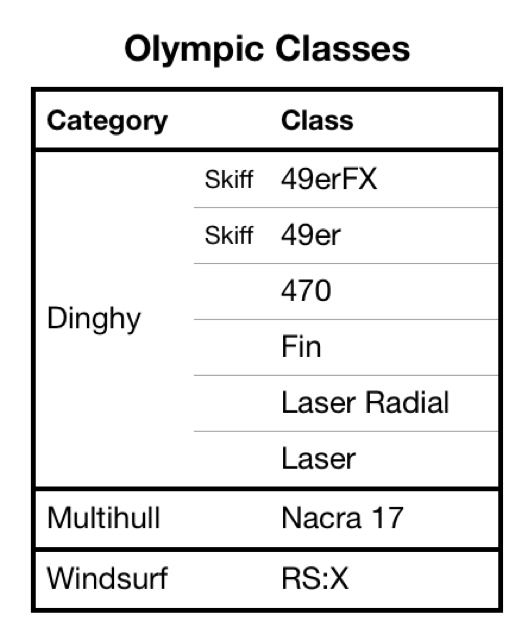
\includegraphics[width=0.32\textwidth]{olym_classes.png}
  \caption{Olympic classes \cite{sailoly}.}
\label{fig:olymp_cla} 
\end{figure}

The competition in each class stands for many races and days where the configurations of the course vary according to the environmental conditions. In each race, points are given according to its arrival position; the faster, the lower the score. The winner is the one with the lowest score. Under this competing format, athletes and coaches confront distinct scenarios for which they take different decisions at the starting line. One of these decisions refers to the initial sailing direction. Its importance is related to the configuration of the course.\par 

\section{Competition Course}\label{tracks}
The most common form of a sailing competition is the fleet racing where all participants race around a course and start at the same time along with a line. Here, not only is the reaction time important but the direction that allows the maximum speed that could be attained is too. Usually, two different types of courses take place in the Olympic classes. Figure \ref{fig:trap_c} shows the singular trapezoid course which is defined by a separate start and finish line and 4 points around (buoys); these 6 elements define the legs of the competition, the first leg is the longest one and it is running against the wind.
The trapezoid course is the most completed format courses, the other formats are a partial representation of it, considering only some legs which are already represented in the trapezoid course.\par 
%The other course is the windward/leeward, figure \ref{fig:wl_c} this is simply a two-leg race orientated in such way that the first leg is sail against the wind (called a beat) and the second leg is sail with the wind (called a run). If boats are sailing neither with nor against the wind, the leg is called reach. 

The courses characteristics and conditions of race are also subject to change every 4 years. For example, the current course is regulated as follows \cite{race_pol}: The length and angles of each leg are defined in such way that the course could be completed in maximum 1 hour and the trapezoidal course can be contained in a grid size of 2km by 2km.  Another consideration is the area of the course,  which most of the time is expressed in nautical miles (nm).Figure \ref{fig:olymp_areas_rio} is an example of how the sailing areas are defined by a circular area, within this circle the trapezoid should be located. \par 
Furthermore, the wind conditions refer to the average wind speed in addition to its shift direction. The current regulation establishes that the race will not start if the average wind speed is less than 4 knots(kn)[2 m/s] or more than 25 knots(12.86 m/s) over the entire course, with maximum wind shift of 10$\deg$. 
If wind conditions are not meet the race could be delayed, and if the race has already started, it is possible a change in the course or an abandonment of the race \cite{race_pol}. Because of this, it is clear how important the wind is for sailing; however to understand how it interacts with the boat and the athlete, firstly it is required to know the physics of sailing. \par 
\begin{figure}[ht]
\centering
 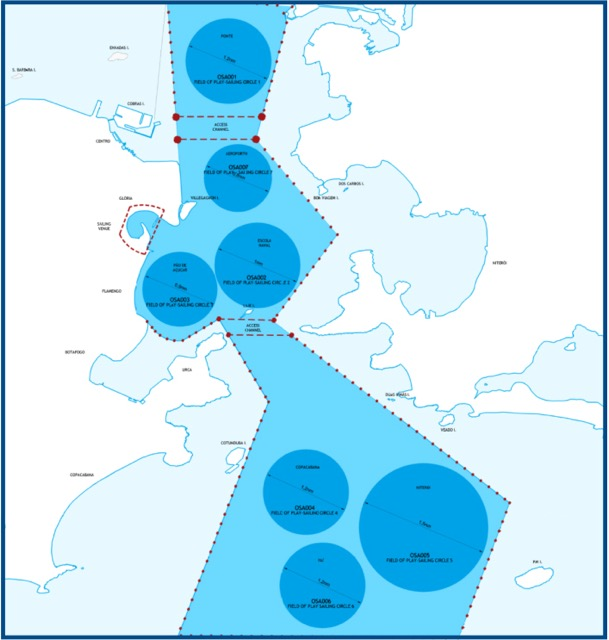
\includegraphics[width=0.6\textwidth]{16_OG_RaceAreasNOR.jpg}
  \caption{Sailing Races Areas. Olympic Games Rio 2016 \cite{instr_rio}.}
\label{fig:olymp_areas_rio} 
\end{figure}

\begin{figure}[ht]
  \centering
  \subfloat[Trapezoid Course ] {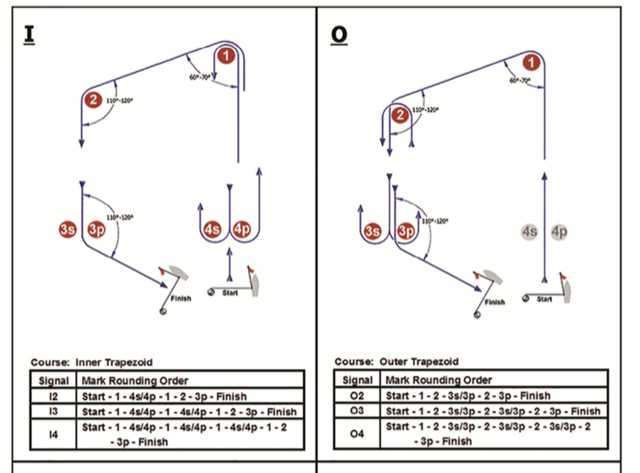
\includegraphics[width=0.53\textwidth]{trap_course.png}\label{fig:trap_c}}
  \hfill
  \subfloat[Windward / leeward course] {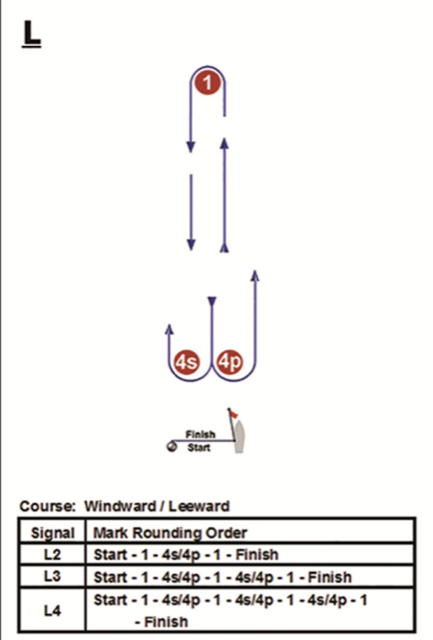
\includegraphics[width=0.25\textwidth]{l_w.png} \label{fig:wl_c}}
  \caption{Types of courses \cite{instr_rio}.}
\label{fig:typecourses} 
\end{figure}

The direction of the boat in respect to the wind determines the type of maneuvers and trajectory that must be followed. For example, the first leg of the trapezoid course runs against the wind and boats cannot displace towards it. The maneuvers used in this condition is shown in figure \ref{fig:tacking}, the trajectory forms a zig-zag pattern that can be started on the left- or on the right-hand side and each change on the heading direction is known as a tack. \par 

Even when the trajectory looks symmetrical, it is important to remember that the wind is not constant all the time and because during the competition, it is only allowed to have a maximum shift of 10 \degree \cite{race_pol}. It is important to understand how this shift affected the course, therefore the time of the course. So far there is no evidence to accept or reject this symmetric condition. This raises the question of \textit{which direction should be taken when the boat has to run against the wind}, in other words, \textit{which is the path with the minimal time to follow?}. \par \noindent
To answer this question athletes and coaches rely on their previous knowledge and experience to decide which is the starting direction. This previous knowledge is based on geographical characteristics around the area of the course and exposure to the site. Top athletes for the Olympic Games train in the site at least one year before the event.\par 
\begin{figure}[ht]
  \centering
  \subfloat[Tacking Maneuver \cite{denny2009float}.] {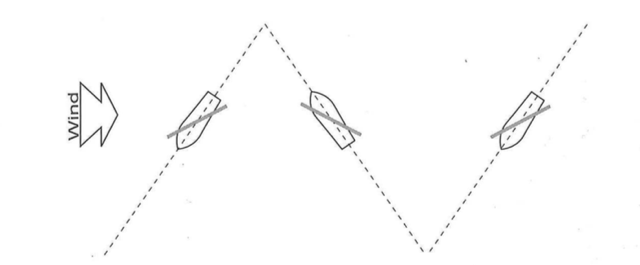
\includegraphics[width=0.65\linewidth]{tacking.png}\label{fig:tacking}}
  \hfill
   \centering
  \subfloat[Tacking maneuver]{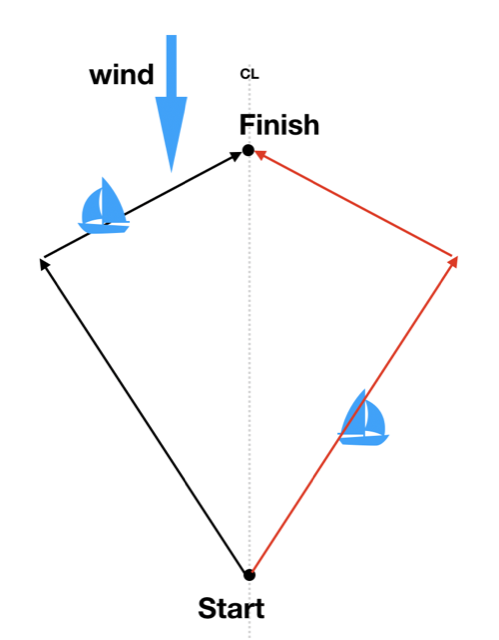
\includegraphics[width=0.3\linewidth]{images/upwind_sym.png}\label{tack_jib}}
  \caption{Tacking maneuver against the wind.}
\label{fig:tack_against_wind} 
\end{figure}

\section{Weather Forecast}
A weather forecast is calculated by supercomputers and updated every certain time according to the regions, usually every three hours. Due to its complexity different agencies and governments have developed models to predict the weather in global terms, so that local predictions could be made. This local predictions take into account the global model and adjusted according to local measurements allowing them to be updated every hour with a grid resolution of 3km by 3km \cite{warner2010numerical}. \par

Uncertain weather is a typical condition that yacht competitions and maritime transportation have to manage. In the case of yacht competitions, courses could take days, weeks or even months; like the \textit{Volvo Ocean Race}, which is an around the world. The path planning for this kind of boats has been researched especially by maritime and logistics sciences, a less number of publications can be found for yacht races and autonomous vehicles, and just a few numbers of researches refer to Olympic races. \par  

 Olympic races have a duration of maximum one hour inside a grid of size 2km by 2km and local forecast is updated every hour within a grid of 3km by 3km. Because of this, the information that coaches and athletes can access previously to the race does not match the characteristics and needs for them at first instance.\par
 Short course and long courses races are different. Short courses, for example, are more sensitive to random fluctuations \cite{philpott2001optimising}. Furthermore, the direction to take at the beginning of the competition could be the optimal just for a couple of minutes but not for the whole race. Time on Olympic sailing classes is critical to winning, but at the same time, a higher resolution on time and space for the weather is more costly in terms of computation effort for weather and the minimal time trajectory processing. The \textit{impact of a fine resolution vs a coarse on the time trajectories is unknown}. In the other hand, it is also unknown \textit{how small this resolution should be} in order to be significant for the  race.\par
 
 \section{The Aim of the Research}
This research proposes an algorithm to model sailing trajectories shaped by wind for Olympic Classes and compare wind models that has different time step and spatial resolutions. Thus this research % which %more specific for Laser (dinghies) competitions %and optimize it to obtain the minimal time for the Laser (Olympic class). 
can answer the next questions, \textit{Which is the optimal sailing route shaped by wind for the Laser (Olympic class) when the time and spatial resolution is set constant for every hour or when it changes every 10 minutes. Which resolution is the most representative and provides accurate results?}. This study suggests that the sensibility of the optimal route due to changes in the wind field and starting direction can define zones and shape the trajectory for minimal time paths. \par 

Moreover, it demonstrates the effects on their resulting trajectories with its times of 4 different time steps and spatial resolutions. This will be done by means of experiments using the optimization of the algorithm proposed. The results(simulations) obtained can be compared against the measurement data of the selected race. In this way, it is possible to identify the size of the differences and quantify the effect of the uncertain weather over the trajectory and times.\par 
%In other words,%the critical variables influenced by the wind that determine it.
%the study seek 
%To answer the question, What is the optimal sailing route for the Laser (Olympic class) shaped by wind. The objective is to analyze the sensibility of the optimal route due to changes on the wind field and start times. This will determine the zones and the shape trajectory of the optimal path. 
%and conditions that shape not only the optimal but the least route also. 
%To answer this question first, the physical model of yachts was reviewed. Despite the similarities between dinghies(Laser boats) and yachts, the physical model was adapted by adding two coefficients related with sails which indicate%the research focusing on dinghies is significantly lower as consequence adaptations have been made to represent
%how different is steering a dinghy from a yacht. Moreover, these adaptations are reflected on the %These adaptations are related with the
%Velocity Prediction Polar (VPP)diagram. By using the VPP and the wind intensity is possible to set the direction at which the dinghy reach is maximum velocity respect to the wind. This approach is known as Velocity Made Good (VMG).%  and to more specific and the use of sails
%Despite the similarities between dinghies and yachts, the research focusing on dinghies is significantly lower as consequence adaptations have been made to represent how it is steering, one of this is related with the VPP's and the use of sails. The same situation happens when the topic of research is related with optimal routes.  Since Olympic sailing is focused on the seamanship, the understanding of physical principals intends to provide or reveal hints that helps them to train and contest effectively regardless the location and routes. \newline

 \section{Terms, conditions, and limitations}
 %This report asses them 
%%these portable designs %the three concepts  

The algorithm developed is limited to dinghies, the smallest and one of the most used boats on the Olympic classes. More specific, the Laser Class with motion over the XY plane. The 2D model proposed was validated by comparing the results of the simulations obtained against the results Laser races located at Hyères, France during 2018.\par \noindent The experiments to see the effects of the time step on the time and trajectory are the three wind conditions: first, a constant wind intensity and direction along the area of the route; the second, considers a forecast wind field as time-space-dependent variable changing every 10 minutes over 1 km by 1km grid size without current and neglecting the wave disturbances and twisting effects on the sail; the last test %condition 
uses the wind measurements taken at 20 Hz during the competition. The algorithm developed is implemented on MATLAB\textsuperscript{\textregistered} and the optimization tool used is \cite{MatlabOTB}.\par 

Olympic Classes like the dinghy is not a widespread research topic. Besides most of the findings related to path optimization for boats are related to cargo ships and vessels, where the main objective is to minimize fuel costs because this ship can be set to navigate at a constant speed. A smaller amount of researches but more related to sports are the ones related to yachts; the influence of the wind is not the same as for the Olympic Classes. \par \noindent 
Another consideration is the movement of the sailor which was not considered as a variable since it was assumed that the athlete is skilled enough to keep the equilibrium of the boat and maximize speed without further complications. In the case of the crew weight, the simulations used the weight proposed by \cite{laser_opt}, which is between	55 and 70 kg.\par 

 \section{Report Structure}
The report is set as follows: chapter 2 refers to basic concepts and physics of sailboat; the forces and equation that governs its motion in general. The validation of the model, and how the wind model is integrated is reviewed in chapter 3. In chapter 4, the optimizer algorithm is explained as well as how the model is implemented with required modifications for the purposes of this research. The obtained results are analyzed in chapter 5; and finally, the conclusions and recommendations are described in chapter 6.\par 

%has been considering in the development of methods for the optimal path.
%The random fluctuation over the time is more sensitive on short courses rather long coursed.
%Taking good decisions on time depends on: the available data and processing time. The processing time refers to the time it takes to converted the available data into meaningful information. These two variables have been approaching by Different researchers to obtain 




%Because of this Philpott \cite{philpott2001optimising} describe a method for each condition to figure out the optimal path.  The weather variables in a short courses were considered to have a minimum spatial variation, although they enclose a random component due to its dependence over time.\\


%With this method the area and time have to being discretize, more over the it consider different states or possibles angles at which the wind will be directed. Which means that each location has to evaluate each of the states and find the optimal path among  \textit{n} stages.  The larger or the smaller the the discretization the more locations to solve according each stage, which seem that the computational effort will grow considerably since each leg has to be evaluated.  The paper does not mention the computational effort nor the difference of time that can be achieve by using it.Philpott \cite{philpott2001optimising}


%\references{dissertation}
\chapter{The physics behind sailboats} \label{ch:physics_sailboat}

Sailing boats are propelled mainly by wind. However, they displace through the water; in other words, sailboats move through 2 different fluids: water and wind. The mechanics of sailing have been known since the 1950s. Marchaj in 1979 review them and add information which is still being used for yacht design \cite{marchajaereo1979}.\par 

This chapter is focused on the motion of the sailboats, what are the physics concepts behind it, which forces interact in equilibrium and during motion. How the athlete takes part in this model and what other considerations are required to set-up the equations of motion. Since sailboats are governed by similar equations some adjustments are required to differentiate between yachts and lasers, these adjustments are explained on detail on later chapters. \par 
The equations of motion facilitate the identification of variables that can be used as a parameter to model the trajectory as well as to identify its limitations. These considerations are required to optimize the trajectory and obtain a minimal time path. \par
\section{The Interaction between the sailboat, water, and air} \label{sec:interaction_boat_environ}
The origin of the forces and momentum depend on the interaction of the elements of the sailboat with the 2 mediums; water and air. Some of these forces are clear, like the forces acting above the water surface which are produced by the wind and the interaction of it with the sails. These forces have to be balanced by the forces beneath the same surface; in this case, the water interacts with the hull, rudder, and keel. Therefore by adjusting the sail and the rudder, the only movable elements, the sailboat can hold a steady course.\par

Philpott explains how different elements, parts of the sailboat, interact with the surroundings and how they are used to control and attain the equilibrium during motion. Figure \ref{sailboat_terms} shows the most common elements and where are they located. Some of those elements can be manipulated by the seamanship, which means that the variables concerned can be controlled and therefore they are known as control variables \cite{philpott1993yacht}. \par

 \begin{figure}%[ht]
\centering
  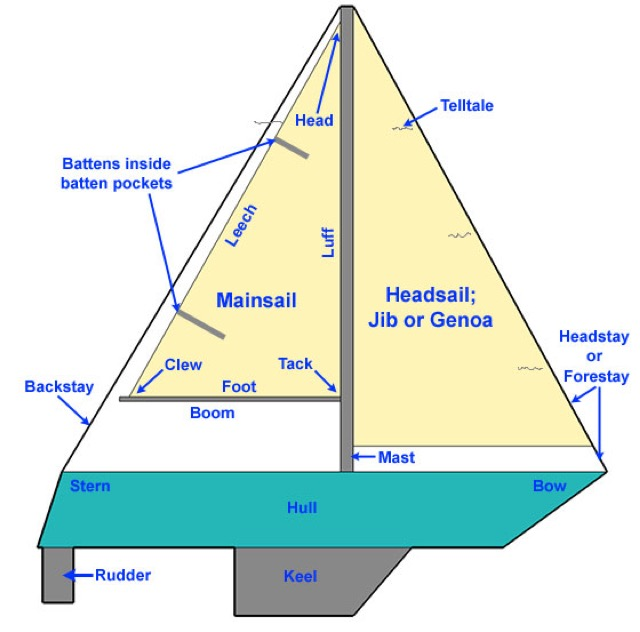
\includegraphics[width=0.4\linewidth]{sailboat_terms.jpg}
 \caption{Common sailboat terms \cite{sailboat_terms}. }
\label{sailboat_terms}
\end{figure}
\nomenclature[S]{$\lambda$}{Leeway Angle}
In order to steer a boat, the seamanship has to control the angle of the rudder, this interacts directly with the current, the direction obtained is called \textit{heading} and these two, rudder and current, generate forces that influence the boat to \textit{yaw}. \par
Due to the wind direction, mainly, the boat slips sideways and this effect is known as \textit{leeway}. The difference in course comparing with the heading is expressed as \textit{leeway angle ($\lambda$)}. %, which can be see in the figure \ref{forces_m} \textit{C}.
The sails adjustment is known as trim; when the trim reduce the area of the sail then the seaman is \textit{reefing}, most of the time this term refers to when the size of the sails is changing.  Reefing under sail allows the seamanship to control the wind intensity. \par
\nomenclature[S]{$M_{R}$}{Righting Moment}
The wind over the sails generates a force and an angle called \textit{heel angle}; which can be seen in figure \ref{forces_m} \textit{B}, this decreases the driving force. Under those circumstances, a moment is generated and to neutralize it, the seamanship generates a \textit{righting moment} (\textit{ $M_{R}$}) by standing on the windward side of the boat to produce it\cite{philpott1993yacht}. 
As a result of these forces, the velocity could be optimal or not. \cite{larsonprinciples} relates the factors and forces proposed in\cite{philpott1993yacht} in terms of forces and resistances, indicating how the dynamics of each of the mediums, water, and air, interact to keep the balance (and be capable to maximize the boat's speed). Therefore, the forces and resistances are related as showed below: \par 
\begin{itemize}  \label{milgramforces}
 \setlength \itemsep{0em}
\item Aerodynamic driving forces = Hydrodynamic resistance;
\item Aerodynamic side force = Hydrodynamic side force;
\item Aerodynamic heeling moment=Hydrodynamic (static) righting moment.
\end{itemize}
An important assumption made by  \cite{philpott1993yacht} and \cite{larsonprinciples} to keep the analysis of the boat in 2 dimensions is that vertical forces are in balance always, same as the pitching moment; Figure \ref{forces_m} \textbf{c} shows the only forces that act when this assumption is made; additionally 2 angles are shown, one of then refers to the wind.\par
\nomenclature[A]{DOF}{Degrees of freedom}
\section{Planes of motion} \label{sec:planes_motio}
Sailing boats are considered rigid bodies that can move in a three-dimensional space; figure \ref{DOF} shows the 6 fundamental types of motion or degrees of freedom (DOF)  with the names and axis where they are referred: three translations and three rotations. \par 
It also shows the water surface which is represented by the plane \textit{XY} and the orientation of the sailboat shows the positive direction of the three axes which follow the right-hand orthogonal system. Thus, \textit{X-axis} is positive in the direction of the motion, \textit{Y} is positive to port or left side of the sailboat and \textit{Z} is positive upwards. In the case of the \textit{Y-axis}, the negative direction or right side of the sailboat is known as starboard.  Besides, for future references, the speed of the boat is along the \textit{X-axis}. These six DOF correspond to three forces and three moments which are going to explain in the next section. \par 
\begin{figure} %[ht]
\centering
  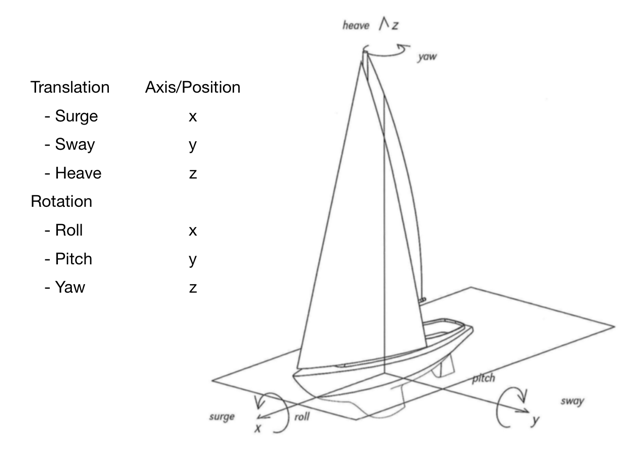
\includegraphics[width=0.7\linewidth]{dof_foss_modif.png}
 \caption{Degrees of freedom of a boat, clockwise reference system \textit{XYZ} \cite{fossati2009aero}. }
\label{DOF}
\end{figure}

%The information provided in the figure %To represent the position, velocities and forces, a set of vectors are defined in 

Because the sailboat interacts between two fluids not only do they generate forces but also resistances in both mediums. It is important to know how the elements are named and which words are related with a specific axis and  %These simple concepts are useful to understand how the equilibrium is generated in the static condition, 
which elements interact on it and how it is conserved when the sailboat moves from one point to another. \par 

\section{Hydrodynamic and Aerodynamic Forces and Momentum} \label{section:forces_moment}
The static and dynamic balance of any type of boat is based on Newton's second law. However, when the boat moves, a dynamic situation, it is the winds' velocity that leads to this equilibrium. Because the sailboat interacts between two fluids they not only generate forces but also resistances.
\nomenclature[S]{$F_{A}$}{Total Aerodynamic Force}
\nomenclature[S]{$F_{H_{TOT}}$}{Total Hydrodynamic Force}
The next equations basically show that the total aerodynamic force ($F_{A}$) is equal and opposite to the total hydrodynamic force ($F_{H_{TOT}}$). \par
From section \ref{sec:planes_motio}, a set of vectors can be defined to represent the position, velocities, and forces. The notation used here is similar to the one used by the \acrfull{sname} %\acrlong{sname} (\textit{\acrshort{sname}})%the Society of Naval Architects and Marine Engineers (\textit{SNAME}) 
because different authors use different notation, this work is intended to stay close to the norm which is shown in table \ref{table:SNAME_notation}, this notation refers to the body-fixed reference frame.
\nomenclature[A]{\textbf{SNAME}}{Society of Naval Architects and Marine Engineers}
\begin{table}%[]
    \centering
    \begin{tabular}{c|c|c|c}
    \hline
          Motion/Rotation & Force/Moment & Linear/Angular vel & Position/Angles   \\
    \hline 
         Surge(X-axis) & X & u & x \\  
         Sway (Y-axis) & Y & v & y \\
         Heave(Z-axis) & Z & w & z \\
         Roll (X-axis) & K & p & $\phi$ \\
         Pitch (Y-axis) & M & q & $\theta$\\
         Yaw (Z-axis) & N & r & $\psi$\\
    \end{tabular}
    \caption{\acrshort{sname}'s notation for motion components \cite{Alves2014ASailboat}}
    \label{table:SNAME_notation}
\end{table}

\nomenclature[S]{$\theta$}{Pitch Angle}
\nomenclature[S]{$\phi$}{Roll Angle}
\nomenclature[S]{$\psi$}{Yaw Angle}

\subsection{Wind and the Velocity Triangle} \label{sec:wind_vel_trian}
\nomenclature[S]{$V_{tw}$}{True Wind Velocity}
\nomenclature[S]{$\beta_{tw}$}{True Wind Angle}
\nomenclature[S]{$\kappa$}{Exponent for wind velocity at different height [1/7,1/4]}
In sailing, the wind is characterized by its speed and direction and it is defined as \textit{true wind velocity ($V_{tw}$)} and \textit{true wind angle ($\beta_{tw}$)}. Because it also interacts with the water surface, in some cases its intensity depends on the height where it was measured, to know its value at a different height it is estimated by equation \ref{eq:wind_h}. According to \cite{claughton1998sailing} the exponent $\kappa$ has a value between 1/7 and 1/14, and; the reference height for measurements is 10m above the water surface. \par 
\begin{equation}\label{eq:wind_h}
    V_{tw}(Z)=V_{tw}(Z_{ref}) \cdot \bigg( \frac{Z}{Z_{ref}} \bigg)^\kappa
\end{equation}

The steady motion of the sailboat not only depends on the balance of forces but also on the relation between velocities, boat, and wind, mainly. This interaction is represented by the velocity triangle shown in figure \ref{vel_triangle}. The triangle introduces the apparent wind velocity ($V_{aw}$) and angle ($\beta_{aw}$).\par 
\nomenclature[S]{$V_{aw}$}{Apparent Wind Velocity}
\nomenclature[S]{$\beta_{aw}$}{Apparent Wind Angle}
%\begin{figure}[ht]
%\centering
%  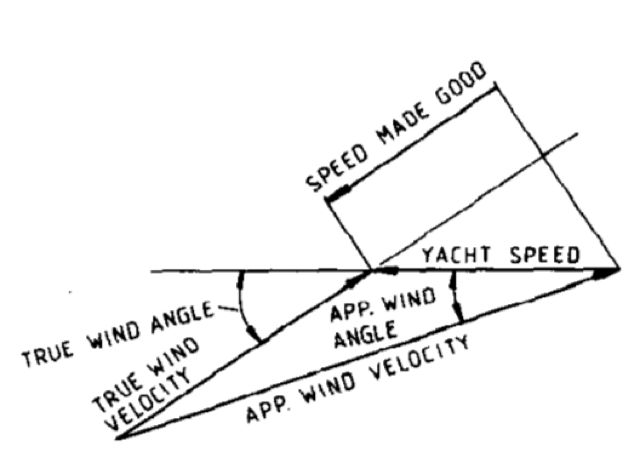
\includegraphics[width=0.65\linewidth]{Larsson_triang_vel.png}
% \caption{Velocity triangle  \cite{larsonprinciples}. }
%\label{vel_triangle_old}
%\end{figure}

%option figure to REVIEW
\begin{figure} %[ht]
  \centering
  \subfloat[Velocity triangle  \cite{larsonprinciples}. ]{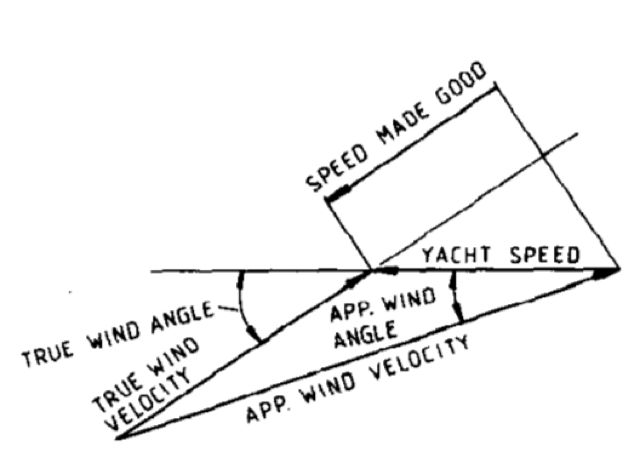
\includegraphics[width=0.45\linewidth]{Larsson_triang_vel.png}\label{vel_triangle}}
  \hfill
  \subfloat[Angles and course direction \cite{marchajaereo1979}.]{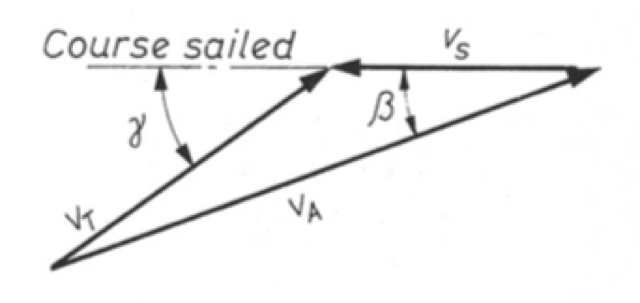
\includegraphics[width=0.45\hsize]{geo_vel_triangle}\label{fig:velTriang_sailCourse}}
  \caption{Velocity Triangle and angle directions of wind and $\lambda$  \cite{marchajaereo1979}, \cite{larsonprinciples}.}
\label{fig:Vel_Trian_Ang} 
\end{figure}

\nomenclature[S]{$V_{aw}$}{Apparent wind velocity}
%\nomenclature[A]{SGP}{Some Random Acronym}
%\newacronym{gcd}{GCD}{Greatest Common Divisor}
%EXAMPLE \acrlong{gcd} \acrfull{gcd} \acrshort{gcd} \acronymtype 

\nomenclature[S]{$\Theta$}{Heel Angle}
\nomenclature[S]{$\gamma$}{Course Angle}
\nomenclature[A]{$CE$}{Center of Effort}
\nomenclature[S]{$V_{boat}$}{Boat's velocity}

The $V_{aw}$ and $\beta_{aw}$ result from the vector summation of the true wind ($V_{tw}$) and sailboat's ($V_{boat}$) velocity, \ref{eq:vel_appVector}; a more complete estimation of them uses the heel angle ($\Theta$), equations \ref{eq:app_angle} and \ref{eq:app_angle} show how to calculate them. These equations include the heel angle because $V_{aw}$ is used to calculate some sail force coefficients which are specified at the center of effort (\textit{CE}), its location is about 40\% at the mast height. The $\beta_{aw}$ incorporated the leeway angle ($\lambda$), which value is usually less than 6\degree \cite{philpott1993yacht},\cite{claughton1998sailing}. Subsequently, the course angle $\gamma$ is complementary to the $\beta_{aw}$ when $\lambda$ is not bigger than 6\degree \ref{fig:velTriang_sailCourse}. \par
\begin{equation}\label{eq:vel_appVector}
    \vv{V_{aw}}=\vv{V_{tw}}-\vv{V_{boat}}
\end{equation}

\begin{equation} \label{eq:app_angle}
    \beta_{aw}=tan^{-1} \bigg( \frac{ V_{tw} sin \beta_{tw} cos \Theta }{ V_{tw} cos \beta_{tw} + V_{boat}} \bigg)
\end{equation}
\newline
\begin{equation} \label{eq:ap_vel}
    V_{aw}=  \sqrt{ (V_{tw} sin \beta_{tw} cos \Theta)^2 + (V_{tw} cos \beta_{tw} + V_{boat})^2}
\end{equation}

\subsection {Equilibrium Equations} \label{sec:equil_equat}
In the static condition, equilibrium is reached when the summation of all the forces and momentum equals zero. In figure \ref{forces_m} these forces are located according to the planes where they act, the names of them and the fluid that drives them. In addition to the forces and momentum, there are 4 angles to consider. Another observation is how the position and weight of the athlete are incorporated in the equilibrium equations. \par 

\nomenclature[A]{$\textit{F}$}{Force}
\nomenclature[S]{$F_{R}$}{Driving Force}
\nomenclature[S]{$R$}{Water Resistance}
\nomenclature[S]{$F_{H}$}{Heeling Force}

The equations of forces(\textit{F}) by plane in equilibrium are:
\begin{equation}\label{eq:force_x}
    \text{(Surge, x  \space axis)  \space} F_{R}=R \\
\end{equation}
\begin{equation}\label{eq:force_y}
    \text{(Sway, y\space axis) \space } \space F_{H,lat}=F_{S,lat}\\
\end{equation}
\begin{equation}\label{eq:force_z}
    \text{(Heave, z\space axis)  } \space F_{V}=F_{VW}
\end{equation}
And those for the momentum (\textit{M}) in equilibrium are:
\begin{equation}\label{eq:m_x}
    \text{(Roll, x  \space axis) \space } M_{R}=M_{H} \\
\end{equation}
\begin{equation}\label{eq:m_y}
    \text{(Pitch, y \space axis)  } \space M_{PA}=F_{PW}\\
\end{equation}
\begin{equation}\label{eq:m_z}
    \text{(Yaw, z \space axis)  } \space M_{YW}=M_{YL}
\end{equation}

 \begin{figure}[ht]
\centering
  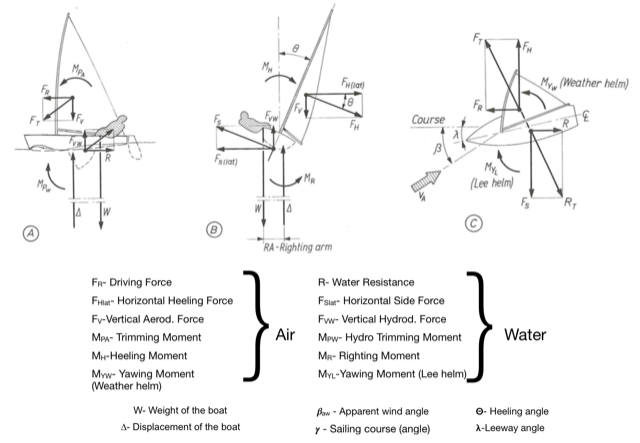
\includegraphics[width=.97\linewidth]{marchaj_forcesM.png}
 \caption{Equilibrium of forces and moments in steady-state sailing condition \cite{marchajaereo1979} }
\label{forces_m}
\end{figure}

\subsection{Aerodynamic Forces and Resistances} \label{sec:aero_forces}
\nomenclature[S]{$F_{S}$}{Hydrodynamic Side Force}
\nomenclature[S]{D}{Drag Force}
\nomenclature[S]{L}{Lift Force}

The force that drives motion of the sailboat is the driving force($F_{R}$); figure \ref{forces_m} \textit{B} shows the force that causes the drift (heel) of the sailboat is the heeling force ($F_{H}$). The motion of the sailboat happens when $F_{R}$ beat the hull resistance (\textit{R}); while in the \textit{ZY} plane the balance of the forces happens when $F_{H}$ equals the hydrodynamic side force ($F_{S}$), which is produced by the effect of the water over the hull. Then:\par 
\begin{figure} [htb!]
    \centering
    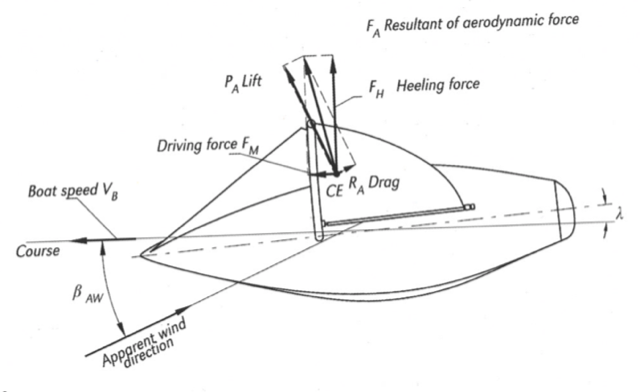
\includegraphics[width=.5\linewidth]{Ftot_aereo.png}
    \caption{Total Aerodynamic Forces \cite{fossati2009aero}}
    \label{fig:Ftot_aereo}
\end{figure}
%( Because $F_{A}$ result from $F_{R}$, parallel to the \textit{apparent wind} direction and $F_{H}$ perpendicular to $F_{R}$. Under balance the variables related to them are:)
\begin{multline}
\\
F_{A}=F_{R}(\parallel V_{aw}) + F_{H}(\bot F_{R} )\\
F_{R}=F_{R}(V_{aw},\beta_{aw}, \Theta) \\
F_{H}=F_{R}(V_{aw},\beta_{aw}, \Theta) \\
F_{S_{lat}}=F_{S}(V_{boat},\lambda, \Theta) \\
R=R(V_{boat},\lambda, \Theta)\\  
\end{multline}
%th they depend on the $V_{aw}$ and $\beta_{a}$; while $F_{S}$ and \textit{R} depend on $V_{boat}$ and $\lambda$. 
Due to the dependency on velocities, $F_{R}$ and $F_{H}$ generate drag (\textit{D}) and lift (\textit{L}) forces acting normal to the center plane of the hull and mast and they are integrated into the forces, figure \ref{fig:Ftot_aereo}, according to \cite{philpott1993yacht} and \cite{claughton1998sailing} as: \par 
\begin{equation} \label{eq:Fr_LD}
    F_{R}=L sin \beta_{a} - D cos \beta_{a}
\end{equation}
\begin{equation} \label{eq:Fh_LD}
    F_{H}=(L cos \beta_{aw} + D sin \beta_{aw}) cos\Theta
\end{equation}
\\ \textit{D} and \textit{L} depends not only on  the sail area (\textit{$A_{s}$)}, $V_{aw}$, and fluid density ($\rho_{a}$), in this case, air, but also on coefficients which depends on the trim and flatness of the sail \cite{philpott1993yacht}, \cite{carrico17symp}, \cite{day2017performance}; these last, are under the control of the seamanship. \textit{D} and \textit{L}  are expressed in those terms as follow: \par
\nomenclature[S]{$\rho_{a}$}{Air Density}
\begin{equation} \label{eq:Lift}
  L=qA_{s}C_{t}  
\end{equation}
\begin{equation} \label{eq:Draf}
    D=qA_{s}C_{d}  
\end{equation}
\begin{equation} \label{eq:dynamic_press}
    q=\frac{1}{2}\rho_{a} V_{aw}^2
\end{equation}
\begin{equation} \label{eq:Cd}
    C_{d}=C_{d}(\beta_{a},trim, flatness)
\end{equation}
\begin{equation} \label{eq:Ct}
    C_{t}=C_{t}(\beta_{a},trim, flatness)
\end{equation}
where:
\begin{itemize} \label{ae_symbols}
    \item $\rho_{a}$ air density approx. 1.225 $kg/m^3$.
    \item $A_{s}$ is the area of the sail.
\end{itemize}

\nomenclature[S]{$A_{s}$}{Sail Area}
\nomenclature[S]{$F_{ms}$}{Driven Sail Force}
\nomenclature[S]{$F_{ss}$}{Side Sail Force}
\nomenclature[S]{$q$}{Dynamic Pressure}

$C_{d}$ and $C_{t}$ values are obtained from tables or graphics and their range is over (0,1), later on, this is going to be explained in detail. \par 
$F_{R}$ is the total force applied on the sail which can be decomposed in 2 more forces; a driven force $F_{ms}$ and a side force $F_{ss}$ expressed in the terms mentioned before as:\par
\begin{equation}\label{eq:drive_sail_force}
    F_{ms}= (L cos \beta_{aw}+ D sin \beta_{aw})cos \Theta sin \lambda + (L sin \beta_{aw}-D cos\beta_{aw})cos \lambda
\end{equation}
\begin{equation}\label{eq:side_sail_force}
    F_{ss}=(L cos \beta_{aw}+ D sin \beta_{aw})cos \Theta cos \lambda - (L sin \beta_{aw}-D cos\beta_{aw})sin \lambda
\end{equation}
%%%NEW SUBSECTION %%%
\subsection {Hydrodynamic Forces and Resistances} \label{sec:hydroforces}
$F_{H_{TOT}}$ is equivalent to $F_{A}$ with the difference that they result from the interaction with the water. In this case, \textit{R}, a drag force (resistance) oppose the motion of the sailboat as shown in figure \ref{fig:Ftot_hydro}; and the horizontal side force $F_{S_{lat}}$, is a lift force acting over the hull and keel. Most of the information related with the modeling of the hull and keel is based on experimental data. % which is used to calibrate the theoretical model.
Then the drag generated by the hull is the result of the  upright, heeled and induced resistances \cite{philpott1993yacht}.\par

\nomenclature[S]{$F_{S_{lat}}$}{Horizontal Side Force}
\nomenclature[S]{$C_{d}$}{Drag Coefficient}
\nomenclature[S]{$C_{t}$}{Lift Coefficient}

\begin{equation}
    F_{H_{TOT}}=R(\parallel( -V_{aw})) + F_{S_{lat}}(\bot R )\\
\end{equation}

\begin{figure}
    \centering
    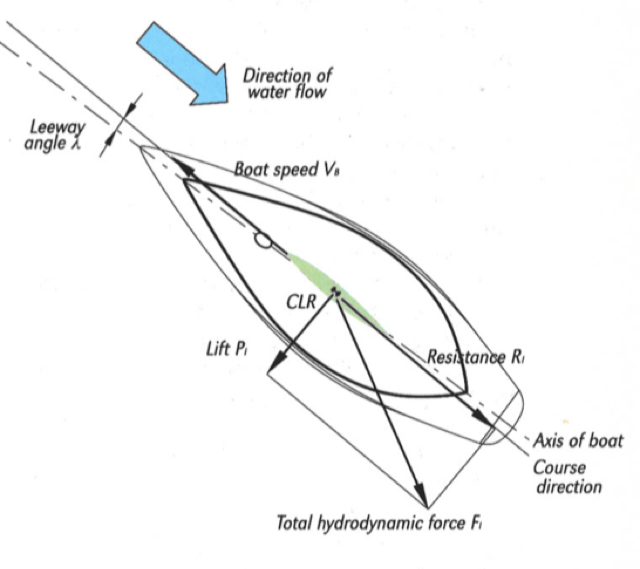
\includegraphics[width=.5\linewidth]{Ftot_hydro.png}
    \caption{Total Hydrodynamic forces. \cite{fossati2009aero}}
    \label{fig:Ftot_hydro}
\end{figure}

The upright resistance is produced by the hull drag and when $\lambda$ is zero. It is constituted by the friction generated by the water viscosity and wave drag, dissipation of energy in form of waves due to the shape of the hull. The formula to calculate these two frictional forces, equation \ref{eq:water_fric} and \ref{eq:wave_fric} is similar to the one from classical hydrodynamics, the difference is the coefficients. $C_{f}$ depends on $V_{boat}$ and its waterline length while $C_{w}$ depends on the hull shape and Froude number (\textit{Fr}), which considers the $V_{boat}$ and length of the sailboat; however, it is often determined by tests evaluations.
\nomenclature[S]{$C_{f}$}{Hydrodynamic Coefficient for the waterline length}
\nomenclature[S]{$C_{w}$}{Hydrodynamic Coefficient for the hull shape}
\nomenclature[S]{$F_{i}$}{Induced and heeled resistance forces}

\begin{equation}\label{eq:water_fric}
 F_{f}=\frac{1}{2}\rho_{w} C_{f} A_{w} V_{boat}^2
\end{equation}
\begin{equation}\label{eq:wave_fric}
 F_{w}=\frac{1}{2}\rho_{w} C_{w} A_{w} V_{boat}^2
\end{equation}
where:
\begin{itemize} \label{R_symbols}
    \item $\rho_{w}$ water density approx. 1000 $kg/m^3$.
    \item $A_{w}$ is the wetted surface area of the sailboat
\end{itemize}
\nomenclature[S]{$A_{w}$}{Wetted Surface Area of the sailboat}
\nomenclature[S]{$\rho_{w}$}{Water Density}

The induced and heeled resistances are combined and related with the heel and $\lambda$, its formula also depends on $V_{boat}$. Due to its complex derivation and different versions the expression is going to be set as; $F_{i}(\lambda,\Theta,V_{boat})$, for the purpose of this work. Then \textit{R} due to hydraulic resistances is calculated as: \par 
\begin{equation} \label{eq:R_total}
    R=F_{f}+F_{w}+F_{i}
\end{equation}

\nomenclature[S]{$S$}{Total Side Force}

In the case of $F_{S_{lat}}$, it depends also on 3 resistances generated by the hull, the lifting surface of the rudder and keel; these 2 last are the more significant and they are also perpendicular to the velocity. This total side force (\textit{S}), on the water plane, depends on the plan area of the keel and rudder and in 2 coefficients, respectively.  Thus, it is estimated as: \par 

\begin{equation} \label{eq:Side_force}
    S=\frac{1}{2} \rho_{w} V_{boat}^2(C_{rudder}A_{rudder}+C_{keel}A_{keel})cos \Theta
\end{equation}.

\nomenclature[S]{$C_{rudder}$}{Rudder Coefficient}
\nomenclature[S]{$C_{keel}$}{Keel Coefficient}
\nomenclature[S]{$A_{rudder}$}{Rudder Surface Area}
\nomenclature[S]{$A_{keel}$}{Keel Surface Area}

The shape, of the rudder and keel, in conjunction with the angle of attack, has implication on each coefficients respectively. %$C_{rudder}$ and $C_{keel}$, each depends on the the shape and angle of attack of each. 
The angle of the rudder ($\beta_{r}$) is the angle it makes with the center line of the sailboat. Each angle of attack (\textit{$\beta_{i_{a}}$})is determined as: \par 
\nomenclature[S]{$\beta_{r}$}{Rudder Angle}
\nomenclature[S]{$\beta_{r_{a}}$}{Rudder Angle of Attack}
\nomenclature[S]{$\beta_{k_{a}}$}{Keel Angle of Attack}
\begin{equation} \label{eq:att_r}
    \beta_{r_{a}}=tan ^{-1} (cos \Theta cos \lambda + \beta_{r})
\end{equation}
\begin{equation}  \label{eq:att_k}
    \beta_{k_{a}}=tan ^{-1} (cos \Theta cos \lambda )
\end{equation}

$F_{S_{lat}}$ in equilibrium can be estimated based by using $F_{H}$ which generates a reaction force below the water surface, then: %
which us know as horizontal side force $F_{S_{lat}}$ and it is determined as follow: \par
\begin{equation}
    F_{Slat}= F_{H}cos \Theta
\end{equation}

%% new section
\nomenclature[A]{$CLR$}{Center of Lateral Resistance}
\nomenclature[S]{$M_{R}$}{Righting Moment}
\nomenclature[S]{$W$}{Weight}

\subsection{Momentum at the sailboat model} \label{sec:momentum_types}
Because $F_{A}$ is applied at \textit{CE}, above the waterline and located over the sails area; and $F_{H_Tot}$ at the center of lateral resistance (\textit{CLR}), defined below the waterline. The moments generated over the sailboat depends on these 4 variables. For example, the \textit{righting moment ($M_{R}$)}, figure \ref{forces_m} \textit{B} is counterbalanced as next: 
\begin{equation}\label{eq:right_mom}
    M_{R}=F_{H}(CE-CLR)_{z}=W \cdot RA
\end{equation}
where:\par
\begin{itemize}
    \item $(CE-CLR)_{z}$ is the heeling arm or the vertical distance between \textit{CE} and \textit{CLR} when $F_{H}$ is perpendicular to it.
    \item W = weight of the boat.
    \item RA = Righting arm or the horizontal distance between the \textit{W} and the \textit{Z} axis.
\end{itemize}
\nomenclature[S]{RA}{Righting Arm}
\nomenclature[S]{$W_{c}$}{Weight of the crew}
This expression does not take into account the weight of the crew. The moment generated by the crew weight is given by the weight of the crew (\textit{$W_{c}$})) and its relative position to the centerline of the boat, which is expressed by a variable known as \textit{$y_{c}$}. This variable has a range value of [-1,1], and if the crew is in the centerline then its value is zero. Another factor to considers is $\Theta$. So the moment generated by the crew according to Philpott \cite{philpott1993yacht} is: \par 
 \nomenclature[S]{$y_{c}$}{Crew position on Y-axis from the centerline}
 \nomenclature[S]{$M_{c}$}{Crew Moment}
 
\begin{equation}\label{eq:Moment_crew}
    M_{c} = y_{c} W_{c} Y_{max} cos \Theta
\end{equation} 
\begin{equation} \label{eq:Mcrew_dist}
    Y_{max} = \frac{1}{2} beam(width)_{sailboat}
\end{equation}

\nomenclature[S]{$M_{R_{TOT}}$}{Total Righting Moment}

and the \textit{total righting moment ($M_{R_{TOT}}$)} is:
\begin{equation} \label{eq:Mr_tot}
    M_{R_{TOT}}=M_{R}(V_{boat}, \Theta, \lambda) + M_{c}
\end{equation}

\nomenclature[S]{$M_{Y}$}{Yaw Moment}
\nomenclature[S]{$R_{hull}$}{Hull Resistance}
The \textit{yaw moment} $(M_{Y})$ causes the rotation on the \textit{Z-axis} and depends on the rudder angle (\textit{$\beta_{r}$}), most of the time, since it can shift the \textit{CLR}, another way to change this distance is by trimming, which changes the area of the sail, therefore, the \textit{CE} shifts its location. If the sailing motion is steady then this moment is zero; otherwise, it can be calculated by the hydrodynamic resistance from the hull and the from the keel and rudder side forces; which are compensated by the sail forces \cite{philpott1993yacht}, \cite{claughton1998sailing}. These 3 forces generated the $(M_{Y})$, as shown next: \par
\begin{equation}\label{eq:Hull_R}
    R_{hull}=R+F_{H}=F_{f}+F_{w}+F_{H}
\end{equation}
\begin{equation}\label{eq:hull_moment}
   M_{hull}=R_{hull}(CLR_{y} cos \lambda sin \Theta - x_{y} sin \lambda cos \Theta) 
\end{equation}
\begin{equation}\label{eq:keel-rudder_moment}
   M_{k-r}=\frac{1}{2}\rho_{w} V_{boat}^2(C_{rudder}A_{rudder}x_{r}+C_{keel}A_{keel}x_{k})cos \Theta cos \lambda
\end{equation}
\begin{equation}\label{eq:sail_moment}
    M_{sail}=x_{s}F_{ss}+z_{0}r sin \Theta F_{ms}) cos \lambda
\end{equation}

\nomenclature[S]{$x_{y}$}{Distance of the CLR from the \textit{Z-axis}}
\nomenclature[S]{$x_{r}$}{Lever Arm of the Rudder}
\nomenclature[S]{$x_{k}$}{Lever Arm of the Keel}
\nomenclature[S]{$x_{s}$}{CE distance from the yaw axis (Z-axis)}
\nomenclature[S]{$z_{0}r$}{Lever Arm of the CE}
\nomenclature[S]{$r$}{Reefed/trim proportion of the sail}
\nomenclature[S]{$z_{0}$}{Height of the CE}
\nomenclature[S]{$M_{sail}$}{Total Sail Moment}
\nomenclature[S]{$M_{hull}$}{Hull Moment}
\nomenclature[S]{$M_{k-r}$}{Moment produced by the keel and rudder}

The \ref{eq:hull_moment} uses $x_{y}$ which refers to the distance of the \textit{CLR} from the \textit{Z-axis} (\textit{yaw axis}) while in \ref{eq:keel-rudder_moment} $x_{r}$ and $x_{k}$ are the lever arms of the rudder and keel, respectively, finally in \ref{eq:sail_moment} $x_{s}$ is the distance from the yaw axis to the \textit{CE} and $z_{0}r$ is the lever arm of it, where $z_{0}$ is the height of the \textit{CE}  and \textit{r} is the reefed/trim proportion of the sail. As mentioned in section \ref{sec:wind_vel_trian} $\lambda$ is small which allows cos and sin functions to be simplified by linear approximations. \par 

\nomenclature[S]{$M_{P}$}{Trimming Moment}
\nomenclature[A]{$g$}{gravity}
\nomenclature[S]{$\Delta$}{Vertical Displacement of the boat, related with the buoyancy when the boat is static}

The \textit{trimming moment} ($M_{P}$) arise from gravity (\textit{g}) and buoyancy forces, the displacement of the boat (\textit{$\Delta$}) is related with $V_{boat}$ ; for example, at high velocities, the lift forces are added to the buoyancy forces at the front sections. 

In case of rough water, however, the pitching motion reduces the speed and it is compensated by the aerodynamic and hydrodynamic forces\cite{claughton1998sailing}.\par 

The equilibrium of forces and moments of the sailboat results from the interaction between the forces generated by the air, or by  water or by both into different parts of the sailboat. These interactions in some cases are sophisticated. One of the reasons is the values that depend on coefficients related with the shape of the particular element of the sailboat and the condition of the wind beside the fact that the density value of each medium is different. The steady motion is reached when all these forces are in equilibrium considering the wind and its direction. Due to the complexity of the relation above the solution or equilibrium condition is not unique. Because of these, it is possible to sail at different directions and to reach a place even when it is on on the windward side of the sailboat. 
%%% NEW SECTION%%%%%
\section{Velocity Prediction Polar} \label{sec:VPP}

\nomenclature[A]{$VPP$}{Velocity Prediction Program/Polar}

In 1979 scientists developed the velocity prediction  program (\textit{VPP}) with the objective to predict the sailboat speed and direction for any wind condition, magnitude, and direction \cite{larsonprinciples}. The results can be interpreted easily using a polar diagram or by reading its results in the form of tables.  The kinetics of the sailboat explains how the motive forces from sails equal the hull resistance and how side forces from keel and rudder equal the sail side forces; in other words, how the aerodynamic forces and momentum are counterbalanced by the hydrodynamics of it. These relations and results are obtained from the static equilibrium equations mentioned in section \ref{sec:equil_equat}.\par 
\begin{figure}
    \centering
    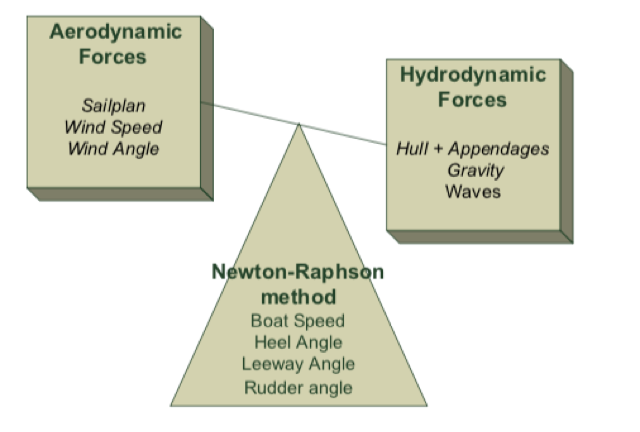
\includegraphics[width=0.5\hsize]{images/Vpp_balance_eq.png}
    \caption{VPP Force Balance Representation \cite{bohm2014velocity} }
    \label{fig:my_label}
\end{figure}
The VPP contains the solutions of the equations to accomplish this balance and it requires not only to solve the hydrodynamic and aerodynamic equations but also to know the properties of the sailboat related with its stability, such as $\lambda$ \cite{larsonprinciples}, \cite{milgram1998fluid}. The information required to get a VPP comes from different sources and all the variables involved can be classified in 4 categories or groups, according to \cite{philpott1993yacht} these groups are:
\begin{itemize}
    \item design (\textit{$_{d}$}): describe the size and shape of the sailboat and its elements.
    \item environment (\textit{$_{e}$}): describe the wind and current in which the sailboat will perform.
    \item control (\textit{$_{x_{c}}$}): these are setting variables that can be adjusted within some limits or constraints by the seamanship, such as $\beta_{r}$, $y_{c}$, \textit{f}, and \textit{r}.
    \item behavior (\textit{$_{y_{b}}$}): these variables describe the motion or condition of the motion at a given time or due to a given environmental condition. Examples of this type or variables are: $\lambda$, $\beta_{tw}$, $\Theta$, and the $V_{boat}$
\end{itemize}

\nomenclature[S]{$_{d}$}{Subscript for Design Variables}
\nomenclature[S]{$_{e}$}{Subscript for Environment Variables}
\nomenclature[S]{$x_{c}$}{Subscript for Control Variables}
\nomenclature[S]{$y_{b}$}{Subscript for Behavior Variables}
\nomenclature[S]{${aux}$}{Subscript for Auxiliary Variables}

The rest of the variables can be grouped as \textit{auxiliary} variables (\textit{$_{aux}$}). These variables describe transitional stages or intermediate calculations, such as $V_{aw}$, \textit{D}, \textit{L}, $M_{c}$, $M_{sail}$ among others. The arrangement of these groups results in at least 22 simultaneous nonlinear equations which can be solved by specifying a performance criterion and optimizing the \textit{$_{y_{b}}$} variables.
%From the equations of previous sections 18 variables were identiy as \textit{aux}.  
 
Because VPP plots are symmetric only half of it is usually represented as shown in figure \ref {typ_vpp}. The polar diagram indicates the wind direction or \textit{true wind angle} at 0\degree , $V_{boat}$ is defined by the radius size of the concentric half circles, the straight lines indicate the direction of the boat from the wind direction. Last, the wind speed is the group of lines that form a half heart shape; the intersection of these lines with direction lines indicates the maximum velocity that a sailboat can attain. \par 
\begin{figure} %[ht]
  \centering
  \subfloat[VPP plot for true wind angles from 0 \degree to 180\degree and true wind speeds from 4 to 10 m/s (7.77-19.44 kn) \cite{larsonprinciples}.]{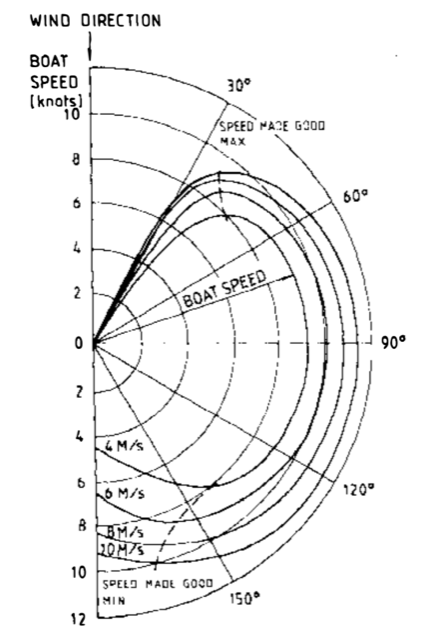
\includegraphics[width=0.38\linewidth]{vppLarsson1990.png}\label{typ_vpp}}
  \hfill
  \subfloat[Polar Curve of the Propulsion System \cite{yang2011control}(Full VPP representation).]{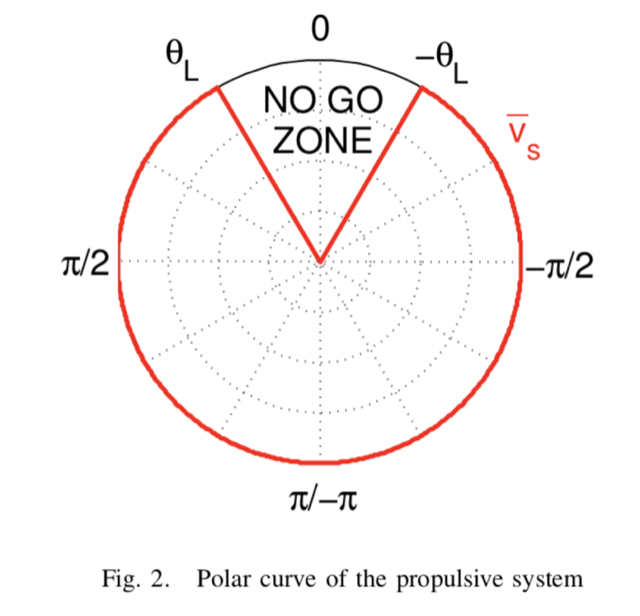
\includegraphics[width=0.45\hsize]{no-go_zone_yang.png}\label{no_go_zone}}
  \caption{VPP diagram}
\label{vpp_diag} 
\end{figure}

By using the VPP not only the direction of the maximum sailboat speed can be identified but also it shows the direction where the speed is the slowest. The angle range of this speed or speeds corresponds to the concave curve of the true wind, the area is defined as the \textit{no-go-zone} and it represents the set of directions that should be avoided to stay away from the irons \cite{yang2011control},\cite{denny2009float}, which means that under these directions the sailboat  motion is minimal, its propulsion is no enough or minimal to outweigh the resistance derived from the hull and sail.\par 

The performance criterion most used is to maximize $V_{boat}$ except when the sailing is towards the wind, upwind condition or sailing to windward. In this case, the performance criterion change from velocity to the distance that can be travel during a certain time.  This criterion is known as the velocity made good \textit{(VMG)} and it indicates where the sailboat is on the space from a reference and how is its motion \cite{larsonprinciples}, \cite{marchajaereo1979} \cite{philpott1993yacht}. \par 
\noindent
\textit{VMG} is determined by equation \ref{eq:VMG}. This relation can also be found in the velocity triangle, figure \ref{vel_triangle}, a more detailed geometrical is the figure \ref{fig:vmg_marchal_book}, where it is possible to identify how the $\beta_{tw}$ and $\lambda$ interact to gets the $\beta_{aw}$ therefore, how distance from the origin or reference point can be optimized and how different angles perform with the same given time. \par
\nomenclature[A]{$VMG$}{Velocity Made Good}

\begin{equation}\label{eq:VMG}
\begin{aligned}
VMG &=  \mid V_{boat} cos \beta_{tw} \mid 
\end{aligned}
\end {equation}

\begin{figure}
    \centering
    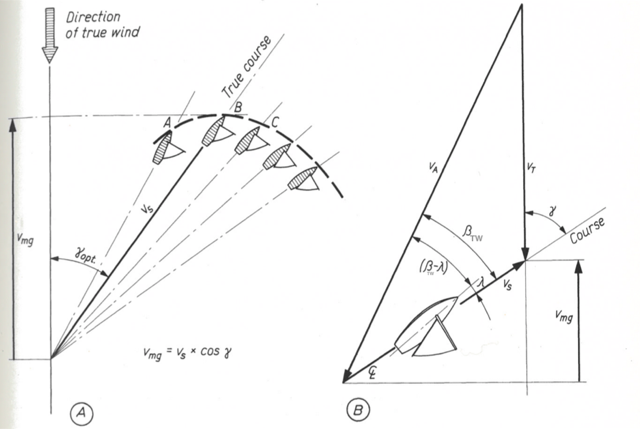
\includegraphics[width=0.75\linewidth]{vmg_marcha.png}
    \caption{Definition of VMG. A. VMG at  different angles. B. Velocity triangle including the leeway angle \cite{marchajaereo1979}.}
    \label{fig:vmg_marchal_book}
\end{figure}

The VPP is obtained by balancing the equations from previous sections, from equation \ref{eq:force_x} to equation \ref{eq:sail_moment}. It derives the $V_{boat}$ at different wind conditions and at different directions, angles respect to the wind. 

However, these equations are not usually solved in its six DOF. Because it was assumed that the vertical forces and moments are always in equilibrium, as was mentioned by \cite{larsonprinciples}, \cite{fossati2009aero} and on section \ref{sec:interaction_boat_environ}. The VPP partially solves the equations which means that the result provided only applies on 2D; particularly in the plane \textit{XY}. So it only considers the rolling moment and longitudinal forces  because changes on the \textit{Z} plane are neglected; but some of the variables related with the \textit{Z-axis} are considered, like $\Theta$. \par 
In this section, it was identified how the variables are categorized, most importantly which variables can be adjusted by the seamanship and which are defined by the sailboat and weather.


\section{Equations of Motion} \label{sec:eq_of_motion}
The motion of the boat from one point to another occurs in the XY plane. In the previous sections, the different components like forces generated by the wind and water were explained and how the seamanship or athlete compensate these forces by interacting with sailboat via sails,$\beta_{tw}$, and rudder, $\lambda$, mainly. On section \ref{section:forces_moment} 
it was mentioned that pitching moment and sway forces (vertical forces) are always in equilibrium, which means that heave and  pitch  motion can be omitted and the motion analysis only occurs on the XY plane within 4 DOF. These motions are the surge, sway, yaw, and roll.\par 

In 2004, de Keuning. et. al \cite{keuning2004mathematical} propose a mathematical model to describe the motion of sailboats or \textit{tacking maneuvers} with wide used parameters, like the information provided by the \textit{Delft Systematic Yacht Hull Series} (\textit{DSYHS}), so the estimation of the coefficients can be defined from this model without the need for experimental data for specific sailboat. \par 

\nomenclature[A]{$DSYHS$}{Delft Systematic Yacht Hull Series}

In the model, the main change refers to its coordinate system, figure \ref{fig:csys_tackmodel} shows the that the coordinate system is at the center of the sailboat, the \textit{Z-axis} is positive orientation when it points downwards and the \textit{Y-axis} is pointing at starboard \cite{keuning2004mathematical}. \par

\begin{figure} %[ht]
  \centering
  \subfloat[Motion depict by the mathematical model.]{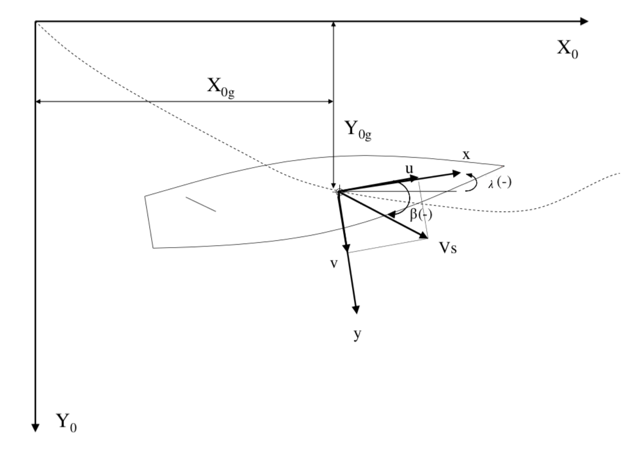
\includegraphics[width=0.38\linewidth]{ridder_motion.png}\label{fig:motion_csys_tackmodel}}
  \hfill
  \subfloat[Angle's location and axis orientation according to the coordinate system.]{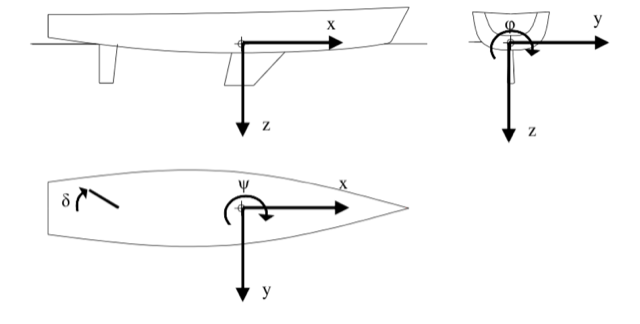
\includegraphics[width=0.45\hsize]{ridder_caxis.png}\label{fig:axis_cystackmodel}}
  \caption{Motion depiction of the mathematical model bestow by the coordinate system \cite{keuning2004mathematical}.}
\label{fig:csys_tackmodel} 
\end{figure}

The next equations or Euler's equations for sailboats motion described by \cite{keuning2004mathematical} define the total forces applied in the sailboat element corresponded to the main axis.\par

\nomenclature[S]{$X_{U}$}{Hull resistance in the upright position on the X direction}
\nomenclature[S]{$X_{i}$}{Forces in X direction of the \textit{i} element}
\nomenclature[S]{$Y_{i}$}{Forces in Y direction of the \textit{i} element}
\nomenclature[S]{u}{Velocity along the X direction}
\nomenclature[S]{v}{Velocity along the Y direction}
\nomenclature[S]{$\Dot{u}$}{Acceleration in the X direction}
\nomenclature[S]{$\Dot{v}$}{Acceleration in the Y direction}

The forces on the X and Y axis are: \\  
\begin{equation}\label{eq:force_X_motion}
    X_{U}+X_{hull}+X_{rudder}+X_{sail}=m_{T}(\Dot{u}-v\Dot{\psi})
\end{equation}
\begin{equation}\label{eq:force_Y_motion}
    Y_{hull}+X_{rudder}+X_{sail}=m_{T}(\Dot{v}-u\Dot{\psi})
\end{equation}
And the momentum on the X and Y axis are: \\
\begin{equation}\label{eq:moment_X_motion}
    K_{hull}+K_{rudder}+K_{sail}+K_{stability}=I_{xx} \Ddot{\phi}
\end{equation}
\begin{equation}\label{eq:moment_Y_motion}
    N_{hull}+N_{rudder}+N_{sail}=I_{zz} \Ddot{\psi}
\end{equation}
%<vertical forces are in balance always same as the pitching moment
where: 
\begin{itemize}  \label{symbols o motions}
 \setlength \itemsep{0em}
\item $m_{T}$ = the total mass of the sailboat not including crew.
\item u = velocity along the X-axis.
\item v= velocity along the Y-axis.
\item $\phi$ = roll angle, related to $\Theta$.
\item $\psi$ = yaw angle. %which is the course angle respect to the wind).
\item $I_{xx}$ = total mass moment of inertia in the roll axis (X.axis).
\item $I_{zz}$ = total mass moment of inertia in yaw axis (Z-axis).
\item K = Rolling moment (X-axis).
\item N = Yawing moment (Z-axis).
\item $X_{U}$ = is the hull resistance in the upright position.
%\item $X/Y_{hull}$ = is the resistance of the hull under the heeled resistance.
\end{itemize}

\nomenclature[S]{$m$}{Total mass of the sailboat including crew mass}
\nomenclature[S]{$K_{i}$}{Rolling moment (X-axis) of the \textit{i} element}
\nomenclature[S]{$N_{i}$}{Yawing moment (Y-axis) of the \textit{i} element}
\nomenclature[S]{$I_{ii}$}{Total mass moment of inertia in the \textit{i-axis}}

It is important to clarify that $\psi$ and $\phi$ are variables that describe the location of the sailboat over an area while and they are related with $\Theta$ and $\lambda$ from the kinematics of the sailboat; because the motion described by Keuning et. al \cite{keuning2004mathematical} includes waves effect because of this there is a difference between $\phi$ and $\Theta$. The heel angle $\Theta$ is the rotation from the \textit{Z} plane in \textit{flat water}; while $\phi$, the roll angle, is $\Theta$ plus the rotation induced by the fluctuations on the front wave \cite{kimball2009physics}, \cite{denny2009float}. \par 
\textit{ $ K_{stability} $ } is the moment generated by the weight when $\Theta$ is not zero; the center of buoyancy (\textit{B}) of the sailboat moves laterally and when its vertical line crosses the midplane of the sailboat creates a metacenter (\textit{M}). The distance between \textit{CG} and \textit{M} is known as the metacentric height, \textit{$\overline{GM}$} ) \cite{patterson2014ship} this displacement generates an oscillation and a mass moment that is calculated as follow:
\begin{equation} \label{eq:k_stability}
    K_{stability}=-mg\overline{GM} sin \phi 
\end{equation}

\nomenclature[A]{$B$}{Center of buoyancy}
\nomenclature[A]{$M$}{Metacenter}
\nomenclature[S]{$\overline{GM}$}{Metacentric Height}
\nomenclature[A]{$CG$}{Center of Gravity}

The rudder and the sail are sailboat elements controlled by the seamanship. 
The rudder produces hydrodynamic forces and momentum, as explained in section \ref{sec:momentum_types}; and the weight of the crew generates a momentum \ref{eq:Moment_crew} 
this momentum can be included on the previous equations by assuming that the centroid of $W_{c}$ is located in the center of gravity (\textit{CG}) and so forth the equations are:\par \noindent
Surge (X-axis):
\begin{multline}\label{eq:force_xMasuyama}
    X_{U}+X_{hull}+X_{rudder}+X_{sail}+X_{V\Dot{\psi}}V\Dot{\psi}\\ =(m+m_{x})\Dot{u}-(m+m_{y}cos^2\phi+m_{z}sin^2\phi)v\Dot{\psi}
\end{multline}
\\
Sway  (Y-axis):
\begin{multline}
\label{eq:force_yMasuyama}
Y_{hull} + Y_{rudder} + Y_{sail} + Y_{\Dot{\phi}} \Dot{\phi} + Y_{\Dot{\psi}} \Dot{\psi} \\ 
=\{(m + m_{y})cos^2 \phi + m_{z} sin^2 \phi \} \Dot{v} + (m + m_{x})u \Dot{\psi} + 2(m_{z} - m_{y}) sin\phi cos\phi \cdot v \Dot{\phi}
\end{multline}
\\
Roll (X-axis):
\begin{multline}
     K_{hull} + K_{rudder} + K_{sail} + K_{stability} +K_{\Dot{\phi}} \Dot{\phi} \\
 =(I_{xx} + J_{xx}) \Ddot{\phi} - {(I_{yy} + J_{yy})-(I_{zz} + J_{zz})} sin\phi cos\phi \cdot \Dot{\psi}^2
\end{multline}  \label{eq:m_xMasuyama}
\newline
Yaw (Z-axis):
\begin{multline}
   N_{hull}+N_{rudder}+N_{sail}+N_{\Dot{\psi}}\Dot{\psi}\\
 = \{ (I_{yy} + J_{yy}) sin^2 \phi +(I_{zz} + J_{zz})cos^2 \phi \} \Ddot{\psi} +2 \{(I_{yy} + J_{yy})-(I_{zz} + J_{zz})\}sin\phi cos\phi \cdot \Dot{\psi} \Dot{\phi}  
\end{multline}\label{eq:m_yMasuyama}
\newline
where: 
\begin{itemize}  \label{symbols_motions2}
 \setlength \itemsep{0em}
\item m = mass of the boat without crew
\item $m_{i}$ = the added masses in \textit{i} direction.
\item $I_{ii}$ = total mass moment of inertia.
\item $J_{ii}$ = total added mass moments of inertia.
\begin{itemize}
    \item i= x,y and z.
\end{itemize} 
\item $X_{V\Dot{\psi}}$, $Y_{\Dot{\psi}}$, $N_{\Dot{\psi}}$  = hydrodynamic derivatives of the hull due to yawing.
\item $N_{\Dot{\phi}}$, $K_{\Dot{\phi}}$  = hydrodynamic derivatives of the hull due to rolling.
\end{itemize}

\nomenclature[S]{$J_{ii}$}{Total add mass moment of inertia in the \textit{i} direction }
\nomenclature[S]{$\Dot{\psi}$}{Angular Velocity in the yaw axis (\textit{Z-axis})}
\nomenclature[S]{$\Dot{\phi}$}{Angular Velocity in the roll axis (\textit{X-axis})}
\nomenclature[S]{$\Ddot{\phi}$}{Angular Acceleration in the roll axis (\textit{X-axis})}
\nomenclature[S]{$\Ddot{\psi}$}{Angular Acceleration in the yaw axis (\textit{Z-axis})}
\nomenclature[S]{$X_{V\Dot{\psi}}$, $Y_{\Dot{\psi}}$, $N_{\Dot{\psi}}$}{Hydrodynamic derivatives of the hull due to yawing motion}
\nomenclature[S]{$N_{\Dot{\phi}}$, $K_{\Dot{\phi}}$}{Hydrodynamic derivatives due to rolling}

By using the last equations it is possible to determine the position of the boat and because the sailboat to model is the \textit{dinghy}, sailed by \textit{professional athletes}, the heel angle is considered small close to 0 ( \textbf{$\Theta \approx$ 0}). This assumption means: \textbf{$X_{hull}$, $Y_{hull}$, some terms of $M_{hull}$ and $M_{sail}$ will be canceled, and the \textit{yaw equation} can be neglected}. The \textit{yaw equation} not only because of the restriction of one boat design but because the athletes keep the balance on this axis; additionally, competitions are regulated in such way that the safety of the participants is not compromised, this last restrict the $V_{boat}$. \par 

With this assumptions the equations of motion can be simplified as: \par \noindent
Surge (x axis):
\begin{equation}
       X_{U}+X_{rudder}+X_{sail}+X_{V\Dot{\psi}}V\Dot{\psi}  =(m+m_{x})\Dot{u}-(m+m_{y})v\Dot{\psi}
\end{equation}\label{eq:Fx_motion}
\noindent
Sway (y axis):\par 
\begin{equation}
\label{eq:Fy_motion}
Y_{rudder} + Y_{sail} + Y_{\Dot{\phi}} \Dot{\phi} + Y_{\Dot{\psi}} \Dot{\psi} 
=(m + m_{y})\Dot{v}  + (m + m_{x})u \Dot{\psi}
\end{equation}
\\
These 2 equations can be reorganized so we can get the accelerations vector of the sailboat. The only decision variable identifies until know refers to $\Dot{\psi}$, which is related to the \acrshort{b_aw}%$\beta_{aw}$
, therefore, the $\lambda$. 
From the equation of section \ref{section:forces_moment} and substituting in equation \ref{eq:Fx_motion} and in \ref{eq:Fy_motion} the previous equations becomes:
\begin{equation}\label{eq:X_tot}
    X_{TOT}=X_{U}+X_{rudder}+X_{sail}
\end{equation}
\begin{equation}\label{eq:X_tot2}
    X_{TOT}=Rcos\psi+F_{R}cos\psi+Scos\psi+
    %-\frac{1}{2}\rho_{w}V_{ac}^2 C_{D,h} +F_{l,r}sin \beta_{ac}-F_{d,r}cos \beta{ac} + F_{l,s}sin \beta_{aw} - F_{d,s}cos \beta_{aw}
\end{equation}
\begin{equation}\label{eq:y_tot}
    Y_{TOT}=Y_{rudder}+Y_{sail}
\end{equation}
\begin{equation}
    Y_{TOT}=F_{R}sin\psi+S sin\psi
    %-F_{l,r} cos \beta_{ac} - F_{d,r}sin \beta_{ac} -F_{l,s}cos\beta_{aw}-F_{d,s}sin \beta_{aw}
\end{equation}

\begin{equation}\label{eq:u_dot}
    \Dot{u}=\frac{X_{TOT}}{m+m_{x}}+v\frac{m+m_{y}}{m+m_{x}} \Dot{\psi}+\frac{X_{V\Dot{\psi}}}{m+m_{x}}V\Dot{\psi}
\end{equation}
\begin{equation}\label{v_dot}
    \Dot{v}=\frac{Y_{TOT}}{m+m_{y}}-u\frac{m+m_{x}}{m+m_{y}} \Dot{\psi}+ \frac{Y_{\Dot{\psi}}}{m+m_{y}}\Dot{\psi}
\end{equation}
\begin{equation}\label{x_dot}
    \Dot{x}=ucos\psi +u_{tw}+u_{tc}
\end{equation}
\begin{equation}\label{y_dot}
    \Dot{y}=usin\psi +v_{tw}+v_{tc}
\end{equation}
where:
\begin{itemize}
    \item $u_{tc}$ = True current velocity in the \textit{X-axis}
    \item $v_{tc}$ = True current velocity in the \textit{Y-axis}
\end{itemize}
From table \ref{table:SNAME_notation} it was defined that $\psi$ is related with \textit(r) the yaw angular velocity, and it defines the position or orientation of the boat, which means that it set the direction of the course ($\lambda$).  $\lambda$ is considered a behavior variable(\textit{$y_{b}$}) in section \ref{sec:VPP}. % it was mentioned 
%that  . One of this variables is $\lambda$,  %one of this variables is $\beta_{r}$ while one of the behaviour variables that describes motion is $\lambda$, 
Because it describes the motion of the sailboat, and the seamanship set the direction, this variable is set as a control variable.\par

This chapter explained how the motion of a sailboat can be determined in 2D with the different types of variables or sources for information. In the next chapter, the environmental variables \textit{e} are going to be explained and how they interact with the equations of this chapter.
%\chapter{Integrating the Weather Model into the Sailing Path Generation}
% Question to answers during the next chapters
%%% Instruments used, set-up, materials
%%Description of the instruments and materials

\chapter{The Weather Research and Forecasting Model(WRF) in the Sailing Path Generation} \label{ch:weatherModel} 

%Introduction
The wind model used in this research is a numerical weather prediction (\acrshort{nwp}) known as the Weather Research and Forecasting Model (\acrshort{wrf}). This particular model has the ability to forecast weather and serves as a tool for atmospheric research. This chapter explains the characteristics of the common weather forecast provided during and before the Olympic sailing races and compare it with the requirements of athletes and coaches. This comparison shows the importance of a customized weather(wind) model and describes its characteristics and limitations. \par \noindent 

For the purpose of this project, the model provided is a \acrshort{wrf} wind model stored in a NetCDF file, while the measured data from past race events is provided in a tabular layout. The last part of the chapter explains the reference frames and their relation with the sailboat velocity.\par

The importance of the wind is not only because it is considered the main propulsion source of the sailboat; but also, because it is the wind which demands changes to the seamanship, like direction on the rudder and sail, to balance the kinematic equations of chapter \ref{ch:physics_sailboat}, and reach the maximum velocity  estimated by the \acrshort{vpp}.In such manner, the seamanship uses the wind information to maximize the velocity of the sailboat by adjusting the direction of the sailboat in a similar way the algorithm for path generation uses that information. \par

\nomenclature[A]{NWP}{Numerical Weather Prediction}
\nomenclature[A]{WRF}{Weather Research and Forecasting Model}

\section{The application of the weather models into Olympic Sailing Races} \label{sec:WindModel_on_Olympics}
%WRF weather models into Olympic sailing races}

A wind model forecast is based on a 3-dimensional time-space model, which can be described as a 4-dimensional model. The resolution of this model or granularity is defined by the size of the data sets that describe it. Moreover, the use of weather models during the summer Olympic Games is not new, but neither widely used. In sailing, the main use of them is as an informative source for the organizers. It helps to warranty the safety of the competitors, like in the Para-Olympic events, and reduce delays due to the wind conditions of the competition  \cite{spark2004wind}, \cite{sheng2009structure}, \cite{golding2014forecasting}. Only \cite{giannaros2018ultrahigh} refers to the \acrshort{nwp} model as a tool to develop a strategic plan to course the race for a sailing team. \par 

Previous to competing, athletes and coaches know the exact location of the sailing area which is enclosed by a diameter of a magnitude between 0.8 and 1.5 nm (1.482 - 2.778 km) and course diagrams \cite{SailRaceRio}. For them, it is important to identify wind patterns, such as average magnitude, direction, the range of variation, the location of vortexes, and even the time of the day when they occur. This information allows coaches and athletes to develop a strategic plan to course the race by avoiding undesirable conditions or to maximize the use of favorable zones.\par

Even when the location, dates and times of the races are known, the wind characteristic and details about the area is still not well understood. The time horizons of local forecasts of short term know as \textit{nowcast} for public access is between 1 to 2 hours as a minimum and up to 6 hours, with a spatial resolution between 40 to 100 km \cite{warner2010numerical}, \cite{kristensen2010weather}. These local predictions use measurements from weather stations or any weather data available around the area of interest and extrapolate in time these conditions; whereas days or weekly forecast can use deterministic predictions.\par

Because sailing Olympic races are set into a grid of 2km with a maximum duration of 1 hour; the public information about wind (weather forecast) does not meet the requirements of the athletes and coaches. As a consequence, customized models have been developed to provide the information required by them. A clear example of this type of models was developed by Giannaros \cite{giannaros2018ultrahigh}, which is defined as a \acrshort{wrf} with \textit{ultrahigh resolution wind forecasting}.\par 

An ultrahigh resolution, a detailed level of granularity, means that the spatial variation captured by the model is in the order of hundred meters in the horizontal plane. In this case, the minimum grid size used was about 200 meters on the area of interest and surrounded by different grid sizes up to 25 km. The vertical dimension was defined by 40 unequally spaced elevations or altitudes; while the duration of the forecast stands for 48 hours starting at 0:00 UTC hours each day with a time interval or time step of 30 minutes. \par \noindent 

Just considering the area of the course which is placed within a grid of 2 km, a model of ultrahigh resolution has a granularity of 10,200 data sets or 39.5$\times 10^6$ data points. The model developed by Giannaros has more data sets since the \acrshort{nwp} model considers a larger area around the races and other factors which will be explained in the next section. Furthermore, it was calculated using 300 computer cores of a high-performance computing cluster and more than 900,000 core hours \cite{giannaros2018ultrahigh}. 

Before \cite{giannaros2018ultrahigh}, only \cite{philpott2001optimising} and \cite{allsopp2000optimal} developed models to include the weather for offshore yacht competitions. Instead of using an \acrshort{nwp} model to determine the wind, each work uses a different stochastic process to calculate it. The details about the discretization of the time were not provided. Only \cite{philpott2001optimising} acknowledged a short-course competition where the Markov process only applied to the wind direction; the granularity of the model was 4000 data sets with a time step of 5 seconds. Other applications of wind models refer to vessels routing where the focus is on fuel costs and other logistics metrics. \par 

The \acrshort{wrf} model can provide the detailed information required by the sailors and coaches of Olympics Classes; however, it demands time and high-performance computing equipment, without considering the preliminary input data and validation process it requires to have a feasible and reliable model to work with. In the other hand, the inclusion of weather models for path generation has not evaluated the sensibility of the trajectory due to the granularity of the model. The next section will provide the details about the \acrshort{wrf} model used for this project as well as its general characteristics. \par 

\section{Components of the WRF Wind Model} \label{sec:WRF_WindM}
Weather models, like wind or current models, are discretized over the space and time because the data is organized into a four-dimensional grid data sets. The most used computer formats to share this type of models are GRIB(.grib) and NETCDF(.nc). The form in which they organize the information may differ but both formats contain the volume representation of the wind model. A straightforward format sometimes used to share the information is the tabular format with all the variables as headers. \par

%\subsection{The WRF Model }
The \acrshort{wrf} is a model that combines global atmospheric models with regional measurements to developed high-resolution models. This means that regional models are inserted within global models, as a result, its range of applications is from meters to many latitude-longitude degrees. The integration allows the identification of small climate variations and other types of phenomena, like precipitations. The incorporation of observable data measured at a constant rate and at known locations given flexibility to the model and unification of the available data \cite{warner2010numerical}. \par

\subsection{Spatial Representation of the Wind Model} \label{sec:Space_WindM}

Weather models are volume representations of a particular region, because of this, it is important to identify the data dimensions, to either manipulate or extract properly the variable of interest, like the wind velocity, if the height does not match the CE of the sail, equation \ref{eq:wind_h} should be used to determine it. \par \noindent

Figure \ref{fig:map_projection} shows the sketches of the most common type of map projection used on atmospheric modeling. The main idea of these projections is that a set of rays coming from the same axis of rotation project points from the sphere into the surface of projection which later can be flattened. The advantage of them is that the angles between curves are preserved and the distance distortions are the same in all directions of a point. The map projection to use depends basically on the latitude of interest \cite{warner2010numerical}. \par

\begin{figure}
    \centering
    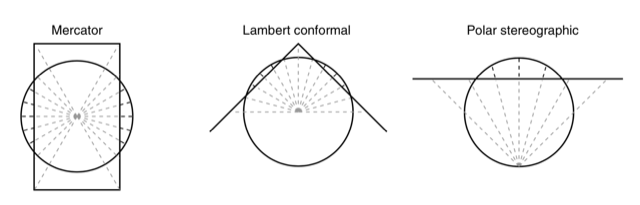
\includegraphics[width=1 \linewidth]{map_proj.png}
    \caption{Most common map projections used on atmospheric models. Mercator is a cylinder projection commonly used for grids in tropical latitudes, Lambert-conformal is a cone, used for mid-latitude grids and the Polar stereographic uses a plane and is used for high latitude grids. The axis of all 3 is always coincident with the Earth's axis. \cite{warner2010numerical}.}
    \label{fig:map_projection}
\end{figure}

The points on the spatial grid of the \acrshort{wrf} model are quasi-regular because the grid is defined by the map projection used. Each intersection of the grid is a data point defined by 4 dimensions (\textit{$n(x_{i},y_{j},z_{k},t)$}) and it represents the location of a variable value. The value of $\Delta x$ is chosen to have a sufficient number of grid points to adequately represent the smallest meteorological feature of interest. \par

Under some circumstances, the model uses a nested approach; where $\Delta x$ is reduced as it gets close to the area of interest. The size of the grid was a crucial concern for \cite{giannaros2018ultrahigh} since the topography of public databases were replaced by new sets that at least match the size of the stipulated grid.\par

\subsection{Time Representation on the Wind Model}\label{sec:Time_onWindM}
The time dimension on the forecast models is limited by the \textit{Courant number} and in consequence with the spatial resolution required. Modifications on the grid have implications closely related with the computational effort; since on each time step the space equations on each grids point have to be solved. The measurement data is another element to incorporate and related to time. \par 

The computational effort for weather models results from the space granularity. Meanwhile, the time step brings stability to the model. Then a small time step provides stable solutions to the equations. While the computational effort is related to the space granularity in a non-linear form. For example, if only one space dimension is double (by a factor of 2), the computational effort time will be 8 times more. \par 

The use of measurement data has an impact on the quality of the results because the rate of their incorporation and values adjust the model forecast. Figure \ref{fig:data_meas_integration} shows how often the measured data is incorporated into the model. This incorporation determines the rate of the re-initialize and the number of cycles within the model forecast that it has to assimilate the observable values. In this form, the measured data not only affects the time of processing but also the accuracy of the forecast. \par

\begin{figure}
    \centering
    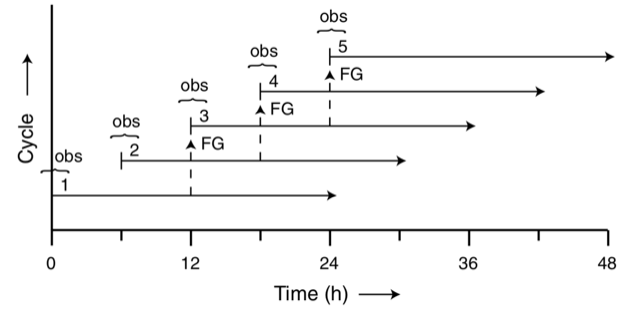
\includegraphics[width=1 \linewidth]{re-run_model.png}
    \caption{Forecast Model with the integration of measured data. During 24 hours, the forecast models are adjusted every 6 hr by the observations. This generates 4 cycles which are assimilated by the model \cite{warner2010numerical}. }
    \label{fig:data_meas_integration}
\end{figure}

\section{The WRF model for the World Cup Series 2018 Hyéres, France}\label{sec:WRF_WindM_FR}

The algorithm for the minimal time path for sailing competitions was developed considering the characteristics of the \acrshort{wrf} wind model on a date of competitions so wind measurements are available. The measurements served not only to set-up the model but also to compare their results. Since \cite{giannaros2018ultrahigh} found that the topography allocation and representation in addition to the initialization of the model have a great impact on the results. \par

The World Cup Series 2018 Hyéres, France Laser competition was chosen. The area where the races took place was named as Echo and the coordinates of its center were: 43\degree 04.144'N, 006\degree 11.913' E. The diameter of the area was 1.6 nm (2.96 km). The date was April 24, 2018. The model forecast 24 hours starting at 0:00 Hrs local time and it was provided by professor Sukanta Basu from the Geoscience Department at TU Delft. \par 
%43,4.144;6,11.913
The information of the wind model was stored in the NetCDF file which is organized in dimensions, variables and attributes defined as data sets \cite{netcdf56302}. In this case, 4 coordinates describe the location and time of the wind velocity. The attributes vector refer to the dimensions of each variable, in this case, the velocity's units were $m \backslash s $. \par 

The wind speed variables were \textit{u} and \textit{v} velocities. Over a rectangle area of coordinates: 41.663\degree N, 4.752\degree E and 44.451\degree N,  7.251\degree  E. The grid size is about 1 km or approx 0.009\degree. The coordinates latitude and longitude where store independently and discretize over a plane of 198$\times$300 elements. \par

The components of the wind velocity were stored on a grid plane of 199$\times$300 for \textit{u} and 198$\times$301 for \textit{v} velocity. This arrangement is known as grid staggering where the different dependent variables are on different grids so the spatial resolution is increasing while the effects of truncation error are decreased. The velocity corresponding to each coordinate is the horizontal average velocity calculated as equations \ref{eq:hor_AVG_velu} and \ref{eq:hor_AVG_velv} indicate.  \par  

\begin{equation} \label{eq:hor_AVG_velu}
    u_{{i,j}_{avg}}=\frac{ u_{i,j} + u_{{i+1},j} } {2}
\end{equation}

\begin{equation} \label{eq:hor_AVG_velv}
    v_{{i,j}_{avg}}=\frac{ v_{i,j} + v_{i,{j+1}} } {2}
\end{equation}

The vertical dimension, height, of the model where discretized over 50 non-uniform steps. The first level corresponds to 7.8 m while the second height is at 25 m. Because the \acrshort{ce} is estimated to be at 2.68 m from the water level \cite{pennanen2015optimal} and the measurements were taken at 10 m above the sea level, equation \ref{eq:wind_h} is used to determine the \acrshort{kappa} value and convert \acrshort{u} and \acrshort{v} fields to the corresponding height. Finally, \acrshort{v_tw} and \acrshort{b_tw} on each grid point can be calculated with equations \ref{eq:v_tw} and \ref{eq:b_tw}, respectively. \par \noindent Equation \ref{eq:b_tw} uses the four-quadrant inverse tangent, (atan2(Y,X)) from \acrshort{matlab} to return values over the [$- \pi, \pi  $] interval.\par 

\begin{equation}\label{eq:v_tw}
    V_{tw_{i,j}}=\sqrt{{u_{i,j}}^2+{v_{i,j}}^2}
\end{equation}

\begin{equation}\label{eq:b_tw}
    \beta_{tw_{i,j}}= atan2d \frac {v_{i,j}}{u_{i,j}}
\end{equation}

The 24 hrs forecast model was discretized in time steps of 10 minutes or ${1} \backslash {6}$ hr. This means that there are 145 steps on the time dimension. Figure \ref{fig:wind_model_FR} shows the wind model provided at 2 different hours, the difference of time is only 1 hour and 10 minutes. The red cross is the center of laser course area named Echo and the black arrows indicate the direction of the wind. The figure also shows the relevance on the scale or granularity; on one side public forecast weather are larger than the one showed here; in the other hand, the interested region is too small even when the granularity was increased significantly. \par    

\begin{figure} [hb!]
  \centering
  \subfloat[Wind model forecast at 10:00 Hrs]{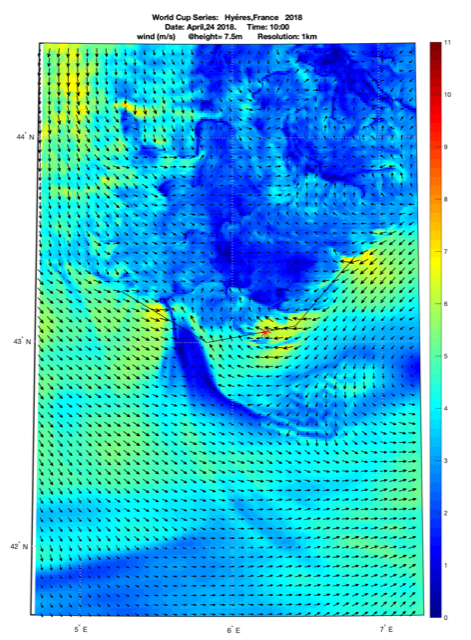
\includegraphics[width=0.5\hsize]{images/fr_10_22.png}\label{fig:fr_10hr}}
  \subfloat[Wind model forecast at 11:10 Hrs]{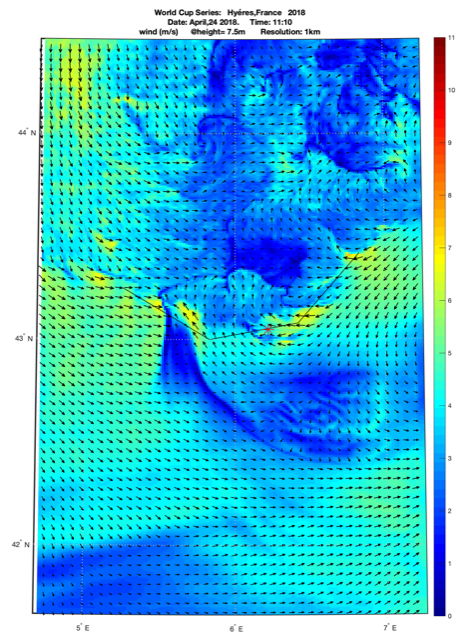
\includegraphics[width=0.5\hsize]{images/fr_11_22.png}\label{fig:fr_11hr}}
  \caption{Wind Model for the World Cup Series 2018 at Hyéres, France. The red asterisk indicated the center of the Echo area for the Laser Course. The area of the model is defined by the corner coordinates at 41.663\degree N, 4.752\degree E and 7.251\degree N, 44.451\degree E.}
\label{fig:wind_model_FR} 
\end{figure}
In summary, the wind model provided is a 4D(\textit{(x,y,z,t)}) grid model of 198 $\times$ 301 $\times$ 50 $\times$ 145 datasets with a space resolution ($\Delta x$) of 1 km and time step ($\Delta t$) of 10 minutes(600 seconds). This kind of granularity is defined as high resolution, and despite the size of the grid the area of competition, its center looks small. This is one of the reasons why \cite{giannaros2018ultrahigh} developed a model with ultrahigh space resolution.\par  

\section{Reference Frames the relation between wind and sailboat velocities} \label{sec:RefFrames}

The wind velocity and direction determines the velocity of the sailboat. However, the wind velocity perceived by the seamanship when the sailboat moves is not the same as the velocity of the sailboat. This perceived velocity is known as the \textit{apparent wind} (\acrshort{v_aw}) and it not only includes the velocity and direction of the wind but also the velocity and direction of the current (\acrshort{v_tc} and \acrshort{b_tc}). The \acrshort{v_aw} and \acrshort{b_aw} are not new concepts, they were introduced on section \ref{sec:wind_vel_trian} and on equation \ref{eq:vel_appVector}. \par

The \acrshort{v_aw} is modified by the current in a similar form as on equation \ref{eq:vel_appVector}, from this equation the current vector is subtracted as shown in equation \ref{eq:vel_wind_current} this velocity is defined as \acrshort{v_awc}. The vector expression shows how different directions influence the results even when the magnitude is the same. On the other hand, if the boat is moving in the same direction as the wind then the apparent velocity increases \cite{denny2009float},\cite{allsopp1998stochastic}. \par 

\begin{equation} \label{eq:vel_wind_current}
\vv{V_{a_{w,c}}}= \vv{V_{tw}} -\vv{V_{tc}} - \vv{V_{boat}}
\end{equation}

However, the previous equation is not the only modification to consider related to wind. %The wind model describes the velocity of the wind 
The wind model only applies over a specific region on the Earth-fixed frame, while the sailboat frame moves along it and is located as indicated by section \ref{sec:eq_of_motion}. It was assumed that the area and the trajectory of the sailboat can be expressed as [\textit{X,Y}] coordinates. This is possible for Olympic Sailing Races because the course area is relative small compared with the total surface of the Earth. Thus to convert the latitude-longitude to [\textit{X, Y}] coordinates, the \acrshort{matlab} function \textit{deg2utm(Lat, Lon)} can be used \cite{allsopp1998stochastic}.\par \noindent 

For the purposes of this research, it is assumed that the Earth circumference is about 40003.2 km. In addition, the nautical mile is one minute (\textit{$1 \backslash 60 \degree$}) of arc on the surface of this sphere, thus the nautical miles is 1852 m. \par 
   
\begin{figure}[hbt!]
    \centering
    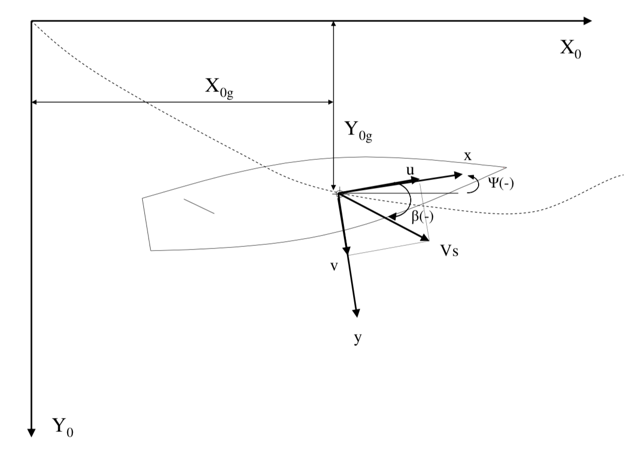
\includegraphics[width=.8 \hsize]{boat_csys.png}
    \caption{Sailboat reference coordinate system and Earth-fixed reference frame \cite{keuning2004mathematical}. }
    \label{fig:boat_Csys}
\end{figure}

Since the sailboat displaces through the horizontal plane of the wind model, another transformation has to be applied in order to describe the motion and forces of the sailboat. Figure \ref{fig:boat_Csys} shows how \acrshort{u} is always aligned with the sailboat mid-plane, therefore to its heading direction (-$\Psi$). The change in orientation respect to the same reference frame is done with the rotation matrix \ref{eq:RotMat}. This transformation is shown in equation \ref{eq:velTransFrame} and it expresses the velocity from the Earth-fixed frame to the sailboat-fixed frame \acrshort{v_btw} \cite{yang2011control}, \cite{bohm2014velocity}, \cite{Alves2014ASailboat}, \cite{keuning2004mathematical}.\par 
\begin{equation}\label{eq:velTransFrame}
    V_{tw}^b= \mathcal{R} \cdot V_{tw}= \mathcal{R}
    \begin{bmatrix}
    u\\
    v
    \end{bmatrix}
\end{equation}

\begin{equation} \label{eq:RotMat}
    \mathcal{R}(- \Psi)=
    \begin{bmatrix}
    cos \Psi & sin\Psi \\
    -sin \Psi & cos \Psi
    \end{bmatrix}
\end{equation}

If the \acrshort{v_tc} is included in the model without waving effects the \acrshort{v_tw} has to be modified before the transformation of equation \ref{eq:velTransFrame}. This is expressed in equation \ref{eq:V_twModifV_C} \cite{allsopp1998stochastic}. However, more equations like the \acrshort{b_aw} and \acrshort{v_aw} have to be redefined because of this inclusion. The equations modified are shown next:\par

\begin{equation}\label{eq:V_twModifV_C}
    \vv{V_{tw,c}}=\vv{V_{tw}}- \vv{V_{tc}}
\end{equation}

\begin{equation}\label{eq:v_twCurBoat}
    V_{tw,c}^b=\mathcal{R} \cdot V_{tw,c}
\end{equation}

\begin{equation} \label{eq:VelCurrWind_boat}
    \vv{V_{aw,c}^b}= \vv{V_{tw,c}^b} - \vv{V_{boat}}
\end{equation}

\begin{equation}\label{eq:b_tw_c}
    \beta_{aw,c}= atan2d \frac {v_{aw,c}^b}{u_{aw,c}^b}
\end{equation}

The transformation of the terms from the sailboat-fixed to the Earth-fixed coordinate system and \acrshort{v_tw} using \acrshort{RM} is not necessary on the equations from \ref{sec:eq_of_motion} since they were already included in their development \cite{keuning2004mathematical}.\par  

\nomenclature[A]{$ MATLAB\textsuperscript {\textregistered}$}{MATLAB R2018b Student License}

\nomenclature[S]{$V_{tc}$}{True Current Velocity}
\nomenclature[S]{$\beta_{tc}$}{True Current Angle}

\nomenclature[S]{$V_{a_{w,c}}$}{Apparent Velocity due to wind and current}
\nomenclature[S]{$V_{tw}^b$}{True Wind Velocity respect to the sailboat}
\nomenclature[S]{$\mathcal{R}$}{Rotational Matrix}
\nomenclature[S]{$\Psi$}{Heading Direction of the sailboat over the horizontal plane}
\nomenclature[S]{$V_{tw}^b$}{True Wind Velocity respect to the sailboat}
\nomenclature[S]{$V_{tw,c}$}{True Wind Velocity affected by true current velocity($V_{tc}$)}
\nomenclature[S]{$V_{tw,c}^b$}{True Wind Velocity affected by $V_{tc}$ respect to the sailboat}
\nomenclature[S]{$V_{aw,v}^b$}{Apparent Wind Velocity affected by $V_{tc}$ respect to the sailboat}

This section explained the \acrshort{wrf} wind model used for the generation of trajectories on Olympic Sailing Races. The characteristics of this model define some of the parameters of the Path Algorithm, therefore for the Minimal Time trajectory. The scale of the Olympic Sailing Courses is small compared with the coverage of wind models, the impact of this coverage hasn't been evaluated and the use of customized models is very limited. Even when the algorithm to develop does not include any model for current, and it is assume that current velocity \acrshort{v_tc} is constant some modifications have to take place. 
% Question to answers during the next chapters
%%% Instruments used, set-up, materials
%%Description of the instruments and materials
%%How the instruments are set-up and what auxiliary connections might need to be used.
%%% add statment
\chapter{The Algorithm to Optimize the Sailing Path for Laser Classes.} \label{sec:AlgOptSail}
%Introduction
The optimization problem for the minimal path is a problem frequently related to logistics and operations research. This problem is usually associated with the \textit{Euclidean} shortest path and solved either with networking optimization or dynamic programming (\textit{\acrshort{dp}}). Although for Olympic sailing classes the optimal path is not related to distance but with time instead. \par \noindent 
Because of this, the research of this type of problem in sports is minimal and it is mainly focused on yacht competitions. Whereas the laser class is the smallest and one of the most used sailboats on Olympic Classes. The objective of this section is not only to explain widely used methods but their elements and how they should apply to develop an algorithm for the Laser Olympic class.\par

Many techniques used on \acrshort{dp} and networking optimization can be used in combination with the \acrshort{vmg} criterion to developed an optimization algorithm for laser races.  Because the target's location and the geometrical domain are the features that allow the use of both criteria thus the optimal solution is found inside the polygon \cite{mitchell2000geometric}.\par 

The first part of this chapter explains how chapter \ref{ch:physics_sailboat} and chapter \ref{ch:weatherModel} are integrated to develop the algorithm to optimize the path of laser boats and obtain a minimal time path. But because most of the formulas on section \ref{sec:equil_equat} are generic, the adjustments required to describe the laser class are explained in the second part of this chapter. Followed by the explanation about the algorithm, details such as the objective function, the constraints, and its validation. The validation of the algorithm is at the end of the chapter, and it provides information about the parameters defined by the user and at the initialization of the algorithm. \par 

%\section{Incorporation of the Wind Model into a Path Algorithm}
\section{Weather Routing Models and Path Algorithms for Sailboats}\label{sec:weatherRoute}

Uncertainty weather is a typical condition that not only yacht competitions have to manage but also maritime transportation. The direction-dependency of the vessel's velocity is seen as a series of regions where the flow's velocity is designed as uniform. This is characterized as an anisotropic medium condition, and path algorithm problems with this characteristic have been solved with different methods \cite{dolinskaya2013fastest}. \par 
\noindent 
The most used methods identified with vessels or yachts and anisotropic medium come from operations research and logistics. For example, from operations research, these methods are dynamic programming (\acrshort{dp}), direct and indirect methods while the networking method is associated with logistics. \cite{kelly2015transcription},\cite{mitchell2000geometric}. In the networking method, the order in which the locations can be reached is not as important than time. \par 
The formulation of the problem is to focus on the time and not in the length of the trajectory. However, it is the velocity of the sailboat the one that determines the direction of the sailboat and considers the wind properties. Because of this, equation \ref{eq:rabaudmintime} defines the time of the path to displace a sailboat between 2 points \cite{rabaudoptimal}. This is the easiest formulation of the problem but it shows how this problem differs from the shortest path approach.  \par

\begin{equation} \label{eq:rabaudmintime}
\begin{aligned}
T_{AB}=\int_{t_{{A}}}^{t_{{B}}} dt=\int_{l_{o}}^{l_{f}} \frac{dl}{v}  \\
\end{aligned}
\end{equation}

\subsection{Dynamic Programming and direction-dependence for Path Algorithms} \label{sec:dynProg}

\acrshort{dp} is a widely used technique to solve the optimal path problem for yachts and maritime transportation. The reason is that it breaks the main problem into multiple stages all connected. In this case, to move from point \textit{A} to point \textit{B} the trajectory is composed for more than two points. Meaning that the main trajectory is assembled by multiple stages or smaller trajectories continuously coupled until it arrives at its final destination. \par \noindent 
The fact that one stage depends on the previous one, allows the recognition of the state of the variables implicated in that solution. This set of state variables is used to optimize the trajectory by iterating each stage until the optimal solution by stage is found. Thus the next stage always starts from the optimal solution given by the last stage \cite{philpott2001optimising}. \par

In yacht competitions and maritime transportation, the trajectory is not only defined by the location of the points but also by the area within they are located. This area has to be defined first and later discretized not only to use variables that depends on its location and time, like wind and current but also to apply \acrshort{dp}. The discretized area is composed of nodes and the line that connects 2 nodes is defined as an arc ($c_{arc}$). For example, node \textit{i} and \textit{j} is connected by the $c_{arc}(\textit{i,j,t(i)})$ which also depends on time (\textit{t}). Since the time at the starting point(\textit{$t_{A}$}) and the wind (\textbf{w}\textit{(i,j,t)}) and current(\textbf{c}\textit{(i,j,t)}) characteristics are known, the minimal time path using \acrshort{dp} is defined in equation \ref{eq:DP_minTimeP_Allsop}  \cite{zyczkowski2017method},\cite{allsopp2000optimal}.

\begin{equation} \label{eq:DP_minTimeP_Allsop}
f^*(i,t)=
\begin{cases}
0,  &  \\
\\
\noindent 
\displaystyle
\min_{j \in \Gamma_{i}} \Bigg[c_{arc}(i,j,t)+f^*\Big(j,t + c_{arc}(i,j,t)\Big) \Bigg]\\
\end{cases}
\end{equation}
\hspace{20mm} otherwise
\begin{equation}
j^*(i,t)=
\noindent 
\displaystyle
arg \min_{j \in \Gamma_{i}} \Bigg[ c_{arc}(i,j,t)+f^*\Big(j,t + c_{arc}(i,j,t)\Big) \Bigg], \quad i \neq n_{finish} 
\end{equation}

The equation explains how the time is minimized at each node until the final destination, point \textit{B}, is reached. $f^*$\textit{(i,t)} is the time at node (\textit{i,t}) which is optimal time resulting from the previous stages. $j^*$\textit{(i,t)} is the next node from \textit{i} on the optimal path, while $\Gamma_{i}$ is the set of subsequent nodes of \textit{i}. The minimal time of equation \ref{eq:DP_minTimeP_Allsop} to move from node \textit{i} at time \textit{t} when the next node is \textit{j} is given by:\par 
\begin{equation*}
    c_{arc}(i,j,t)+f^*\Big(j,t + c_{arc}(i,j,t)\Big) 
\end{equation*}

\noindent
Figure \ref{fig:dp_Allsop} is the graphical explanation of the equation to determine the minimal time from node 1 to 5, starting at time 1 (\textit{n(1,1)}). Node 5 ($n_{5}$) can be reached by 3 different paths, or in other words, there are 3 alternative nodes before $n_{5}$ can be reached.  The nodes 2, 3 and 4 can be reached at different times, the minimum time between them is given by $n_{4}$ with a time of 2 (\textit{n(4,2)}). The next arc is formed from $n_{4}$ to $n_{5}$ and because the starting time of $n_{4}$ is the minimal/optimal time for the first stage, the final time is then the minimum time path from $n_{1}$ to $n_{5}$. \par \noindent
This state-space algorithm for the shortest path includes explicitly the time dimension \cite{allsopp1998stochastic}.

\begin{figure}[hbt!]
    \centering
    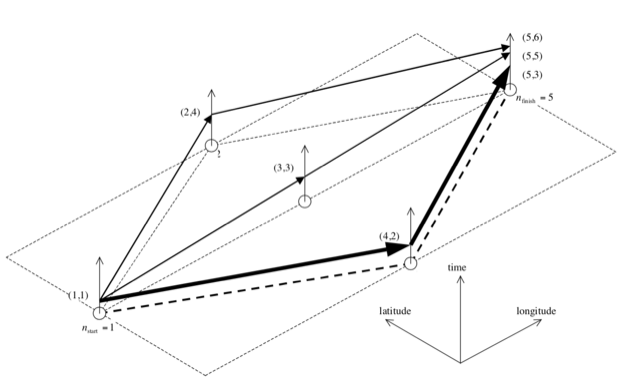
\includegraphics[width=.85 \linewidth ]{Allsopp1.png}
    \caption{Minimal Time Path from node 1 at time 1 (\textit{n(i,t)=n(1,1)}) to node 5 using \acrshort{dp}. The minimal time path to move from node 1 to 5 has gone through node 4 and the path is indicated by the thicker  line \cite{allsopp2000optimal}.}
    \label{fig:dp_Allsop}
\end{figure}
\par 

An alternative process to discretize the area is based on the grid method and the heading decision, which is driven by the maximum velocity of the sailboat. This method can be related to the \acrshort{vmg} criterion because the same distance from the starting point can be reached at different times. Here, the heading-angle decision is discretized by intervals of size $\Delta \Psi$, clockwise and counterclockwise, as a result, multiple sub-routes are generated. If the symmetry of the \acrshort{vpp} is taken into account, some nodes and sub-routes can be represented within a diamond shape \cite{xing2012path} \cite{zyczkowski2017method}. \par \noindent
The number of stages($n_{stages}$) along the straight sailing distance (\textit{L}) between point $P_{0}$ and $P_{n}$ determines the shortest distance between (\textit{L} $\backslash n_{stages}$ ). In this case, $n_{stages}$ can have any value bigger than 1 and it can be seen as the number of attacks that the seamanship could perform. The bigger the number the longer the time of the computational effort to determine the trajectory of the optimal time path \cite{xing2012path}. \par 
\noindent
The optimal heading is finding when the next stage is reached with minimal time. In this case, it is possible that multiple nodes arrive at the same time to the next stage. For this reason, the sub-routes have to been stored and the process continues until the destination point is reached. The algorithm to estimate the minimal time path is similar to the $c_{arc}$ process, the difference is in the form in which the area and stages are determined. The heading-direction approach sometimes uses additional factors over directions where the speed is the maximum. \par

Figure \ref{fig:diamondshape_subR} shows how the heading decision works. In this particular case, e all the sub-routes from $P_{0}$ to $P_{n}$ are contained into a diamond shape. Each node is described by the stage and the node-number per stage, $P n_{stage},i_{sub-route}$ which is determined by the size of $\Delta \Psi$. The nodes over the edges of can only reach the half of nodes compared with the nodes at the center. The number of clear stages represented here is 6 and on each node there a maximum number of sub-routes is 21 and a minimum of 10. It is important to remember here the concept of the \textit{no-go-zone} from section \ref{sec:VPP} because it could reduce the range of the heading direction angle.\par 

%\begin{figure}[hbt!]
%\centering
%  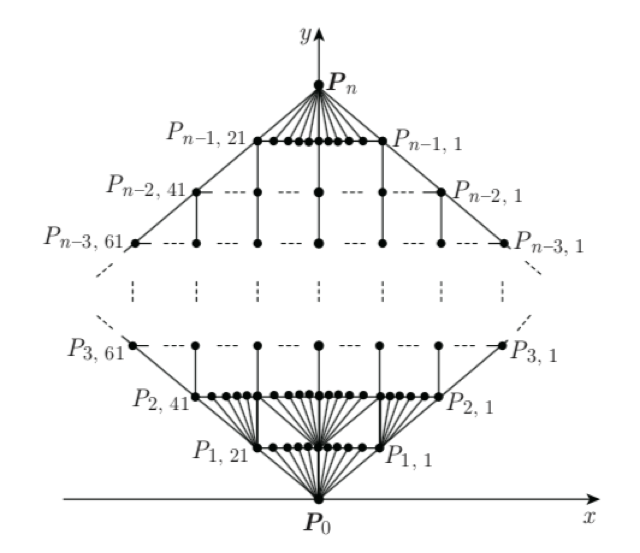
\includegraphics[width=0.6\linewidth]{legyachtxing.png}
% \caption{Leg yatching model \cite{xing2012path} }
%\label{fig:xing_nodesi}
%\end{figure}

\begin{figure} [hbt!]
  \centering
  \subfloat[Sailing Area Discretization for a Sailing Path from point A to B \cite{zyczkowski2017method}.]
  {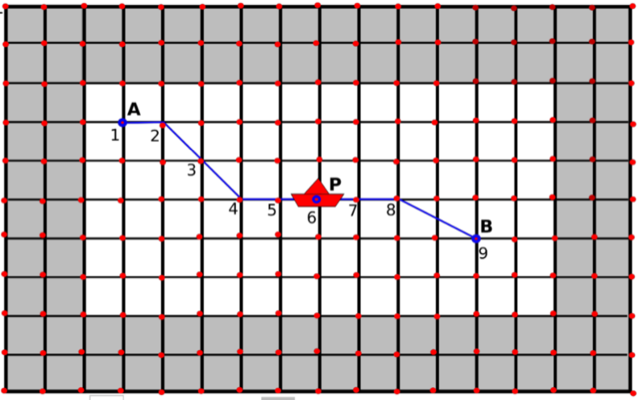
\includegraphics[width=0.33 \linewidth]
  {Sailing_area_heading.png}\label{fig:GridAreaSail}}
  \hfill 
  \subfloat[Heading Directions at a node, 8 angle discretizations \cite{zyczkowski2017method}.]{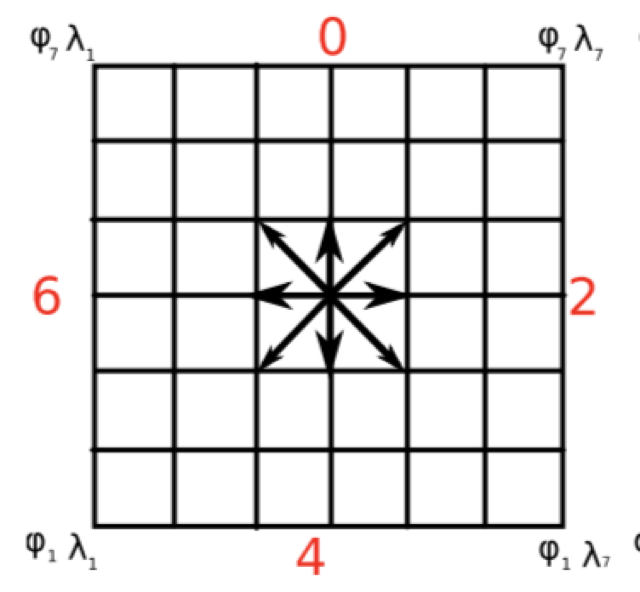
\includegraphics[width=0.22\hsize]
  {HeadDirNode.png} \label{fig:HeadAngle_Discret}}
  \hfill
  \subfloat[Diamond Shape with the Sub-routes for a heading-angle discretization to move from $P_{0}$ to $P_{n}$ \cite{xing2012path}.]
  {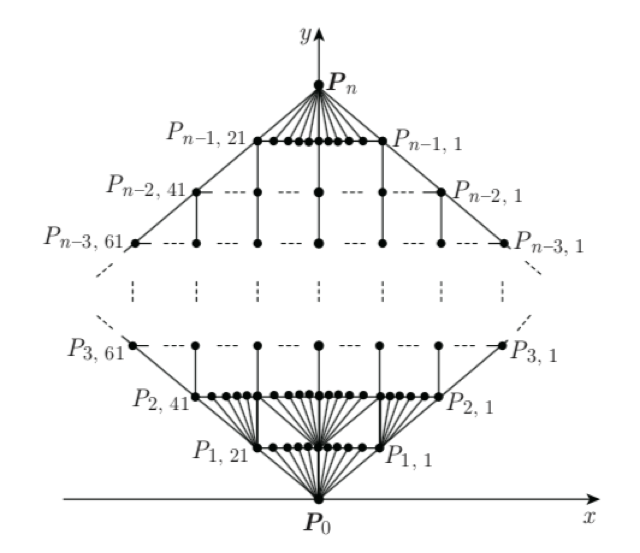
\includegraphics[width=0.33 \linewidth]{legyachtxing.png}
  \label{fig:diamondshape_subR}}
  \caption{Area discretized with a sailing path and Heading Angle discretization}
\label{fig:AreaDiscret} 
\end{figure}

\subsection{Path Algorithm Using Isochrones} \label{sec:isochrones}
A common solution with visual information obtained with \acrshort{dp} in weather routing is the isochrones. The isochrones lines compose a map where each line shows the maximum distance a sailboat can reach during a certain time. Moreover, this map can be seen as the visual representation of the \acrshort{vpp} over different anisotropic media when the weather variation is minimal \cite{allsopp1998stochastic}. \par 
A similar approach relates this type of solution with geometrical optics more specific with wavefronts. This analogy is because the speed of the wavefront depends on the refractive index of the material \cite{rabaudoptimal}. Figure \ref{fig:isochrone_ex} shows how \textit{qtVlm} software uses isochrones to determine the optimal path for a generic yacht.\par

\begin{figure}[hbt!]
    \centering
    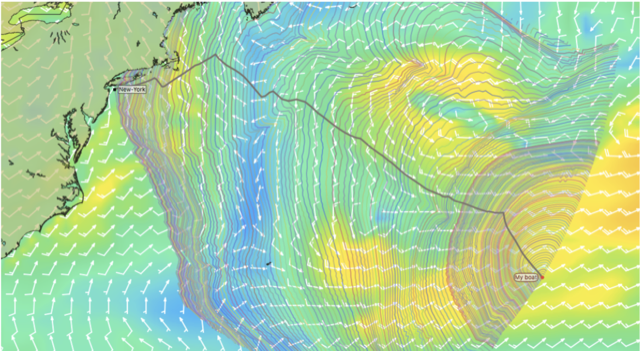
\includegraphics[width=.75 \linewidth]{isochrone_ex.png}
    \caption{Optimal Path Solution from qtVLm software using isochrones for a generic Yacht from a random location over the Atlantic to New York. The optimal path is the gray thick line, the wind direction is indicated by the white arrows \cite{rabaudoptimal}. }
    \label{fig:isochrone_ex}
\end{figure}

The visual information presented by most of these algorithms has been employed by various weather routing software. Despite this, the use of them in sports and in Olympic Sailing Classes is limited. This because they are designed for long-distance yachts races or for maritime-logistics purposes. In both cases, the weather model is assumed to be homogeneous in space and time and frequently loaded from public sources. Meaning that the time step and grid size is much bigger than the required for Olympic Sailing races. Furthermore, when it is used for maritime-logistics purposes the vessels are equipped with communication and other measuring systems that account for weather variations. \par
Despite the advantages of the isochrones techniques and its usage on large course races, the number of application for short courses is limited. The reason is because of the weather is assumed to be perfectly known and even when the \acrshort{vpp} is assumed symmetric the algorithm doesn't explain or shows the limitations of choosing the symmetric path not even as an alternative for some space-time-intervals.\par    

%The envelop shape of the VPP used in \cite{rabaudoptimal} was explained in detail by \cite{dolinskaya2009optimal}.This type of shapes represent a feasible region where a vessel can moves in a straight line in a period of time from the origin; and it was called     \textit{linear path attainable region} for point (0,0)" \cite{rabaudoptimal}.
% resumen 
% points to include use of stages to set the path
% the discretiation of the area, and the wind is assumend location is know
% weather is perfectly know
% alssop interpolation 
% include advantages
\hspace{5mm}
In resume,
%As explained at the beginning of this section
\acrshort{dp} is a flexible method used to find the optimal sailing path and widely used for weather routing. The main characteristics of the previous techniques that have been considered for the development of the laser path algorithm are explained afterward. Before starting any sailing path, first, it is important to define the area within any path might take place. This is not only because of the wind or current model but because inside that area, a set of stages have also to be defined. This area for the sailing path has to cover effectively all the alternatives so the minimal time path can be found. \par 
After the area is defined it has to be discretized, the grid approach is commonly used. By using the grid it is easy to locate the node for either the node or the arc and to find the value for both wind and current. The discretization is directed related to the granularity of the problem and at the same time with the computational effort. \par 
The next characteristics to define is the number of stages is a free number that must be taken with care. The number of stages in combination with the number of variables define the state-space vector. This vector has to been estimated and later on compared as many arcs or nodes were determined. As a consequence of the size of the vector the computational effort can be affected and at this point, the number of operations could grow exponentially.

\section{Adapting the Yacht Model to the Laser Class} \label{sec:laser_yacht}

Most of the research either for path planning or for the physic model for sailboats are associated with the yacht or with bigger boats such as sailing vessels. The figure shows the differences in heights for the mast only, where the AC45 yacht race has a height of 25.5 m while the Laser Olympic class mast's height is 6.1 m. Equations on section  \ref{sec:eq_of_motion} are generic and applicable to any kind of sailboat. Hence to represent properly the laser class some modifications have to made before to properly represent its motion.\par 
\begin{figure} [hbt!]
    \centering
    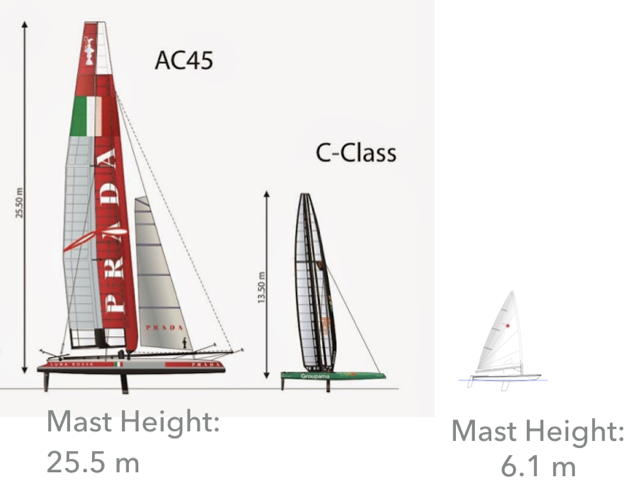
\includegraphics[width=0.74 \linewidth]{yacht_comp.png}
    \caption{Mast Height Comparison between two yachts models AC45 and C-Class versus the Laser Olympic Class, side view. \cite{yacht_compw}.}
    \label{fig:yacht_mast_height}
\end{figure}
The sailboat of the laser class is the dinghy one of the smallest boats propelled by wind, with a maximum weight of 59 kg \cite{sailoly}. Therefore its balance on the \textit{heave axis} (\acrshort{heave_ax}), between the heel angle (\acrshort{heel_ang}) and righting moment (\acrshort{right_m}) is determined by the ability of the crew to adjust its posture over each side of the boat. The posture of the crew respect to the boat is determined by the wind speed and direction mainly. So it can be said that the crew's posture is a response to the weather variations \cite{marchajaereo1979}.\par 

Even when these assumptions are implicit to keep the sailboat analyses in 2-dimensions and developed the \acrshort{vpp} there's is being some discussion about it \cite{philpott1993yacht},\cite{larsonprinciples}. The discussions are associated not only with the posture but also with the impact of the crew's mass (\acrshort{crew_m}). Since for Olympics Sailing Races, it could represent more than $50 \% $ of the total mass of the sailboat (\acrshort{m})\cite{day2017performance}. These without considering the rate of change of these postures adjustments and the assumption that its centroid (\acrshort{crew_m}) is located in the center of gravity (\acrshort{c_g}) of the sailboat. \par 

A deeper analysis and comparison between the adaptations on the standard \acrshort{vpp} were addressed about the coefficients and forces related to the sails. The comparison of the different coefficients values include the data taken from the Offshore Rating Congress (2013) and the observations made in other works \cite{day2017performance}, \cite{carrico17symp}, \cite{binns2002development}, \cite{flay1996twisted}. Furthermore, these modifications correspond to the addition of the \textit{reef} and \textit{flat} coefficients of the sail. Particularly, they account for the fact that dinghy's sail does not reef against strong winds. As a consequence of this, the drag and lift coefficients must be adjusted during the upwind and downwind course \cite{carrico17symp}. \par \noindent
The adaptations directly associated with the 
%were divided according the 
aerodynamic 
%and hydrodynamic 
forces, as a result of the \textit{flat}, \textit{twist} coefficients and the \textit{spill}(\acrshort{spill}) variable 
%were included. 
are showed next. These coefficients model the behavior of the sails and the athlete under strong wind conditions and it includes not only the upwind conditions but also the downwind course \cite{day2017performance}. % in additions to some conditions to be included when a downwind course is sailedIn \cite{day2017performance}. \par 
Therefore, equations \ref{eq:Cd} and \ref{eq:Ct} are modified to account the required adjustments. \par \noindent 
Then \acrshort{spill} modifies equation \ref{eq:Ct} and is shown in equation \ref{eq:liftMod} where \acrshort{Ctwist} has a value of  \textit{8.0} and \acrshort{twist} which is the \textit{twist variable} has a range value of [0,1], \acrshort{CDv} and \acrshort{CLmax} is obtained by interpolation from tabulated values and it depends on \acrshort{b_aw} while \acrshort{CDs} has a value of \textit{0.005} and \acrshort{ARE} is based on the rig geometry and calculated according to it \cite{day2017performance}. \par \noindent  
Equation \ref{eq:Cd} is replaced by \ref{eq:draftMod}, the values taken were the smallest with a reduction of the area of 20 \% to consider shielding from the cockpit \cite{day2017performance}.\par 
%The effective aspect ratio ARE is calculated from the geometric aspect ratio based on rig geometry

\begin{equation} \label{eq:liftMod}
    C_{t}^*=C_{Dv}(\beta_{aw}-s)+C_{Dp}+f^2 \cdot C_{Lmax}^2 \cdot (\beta_{aw}-s) \cdot \Big(\frac{1+C_{twist} \cdot t^2}{\pi AR_{E}} + C_{Ds}\Big)
\end{equation}

\begin{subequations} \label{eq:draftMod}
 \begin{align}
  C_{d}^*= 1.075 && \text{for the frontal area} \label{eq:FrontalAreaDraft} \\
  C_{d}^*= 0.954 && \text{for sideways area} \label{eq:SideAreaDraft}
 \end{align}
\end{subequations}

\par 
The literature regarding \acrshort{vpp} for laser boat classes is limited and it is mainly accounted in \cite{day2017performance}, the comparisons made here are only valid for wind speed between  4 and 16 knots, while races are performed up to 25 knots. This range has to be considered in the development of the algorithm to find the optimal path since it is the velocity of the wind that determines the direction that should be taken in order to maximize the \acrshort{vmg} criterion. \par 

\section{The Optimization Algorithm for the Minimal Time Path}
At this point, all the elements required to define the algorithm for the sailing path have been described. In this section, those elements are going to be implemented in a similar order in which they were described. First, the parameters of the Laser are going to be described so its \acrshort{vpp} can be estimated, then the area for the sailing race has to be defined and finally how the optimization was setting up and validated. 

\subsection{The Laser Olympic Class}
As mentioned before the Laser sailboat is the smallest class of the Olympics Sailing Classes and it is shown in the figure. The dimensions and parameters that describe the laser are regulated by the \acrfull{ilca} and they are shown next in addition to some coefficients previously defined. The figure shows a side view of the Laser Standard and Laser Radial which are Olympic Classes. %For the \acrshort{Asail} and \acrshort{Asail_La} equation is used, where $L_{luff}$ refers to the luff lenght and $L_{foot}$ is the length of the foot, for which the maximum dimensions were used.
%\begin{equation} \label{eq:sail_area}
 %   A_{sail}=0.5 \cdot L_{luff} \cdot L_{foot}
%\end{equation}
\begin{description}
        \item \acrshort{mboat}= 59 [kg] \acrlong{mboat}
        \item \acrshort{Loa} = 4.2 [m] \acrlong{Loa}
        \item Beam = 1.37 [m] Beam width
        \item \acrshort{Tc} = 0.787 [m] \acrlong{Tc}
        \item \acrshort{Asail_La} = 5.76 [$m^2$] \acrlong{Asail_La}
        \item \acrshort{Asail} =  7.06 [$m^2$] \acrlong{Asail}
        \item \acrshort{Ak} = 0.23 [$m^2$] \acrlong{Ak}
        \item \acrshort{Ar} = 0.11 [$m^2$] \acrlong{Ar}
        \item \acrshort{Cdhull} = 0.02 [-] \acrlong{Cdhull}
    \end{description}
\begin{figure} [hbt!]
    \centering
    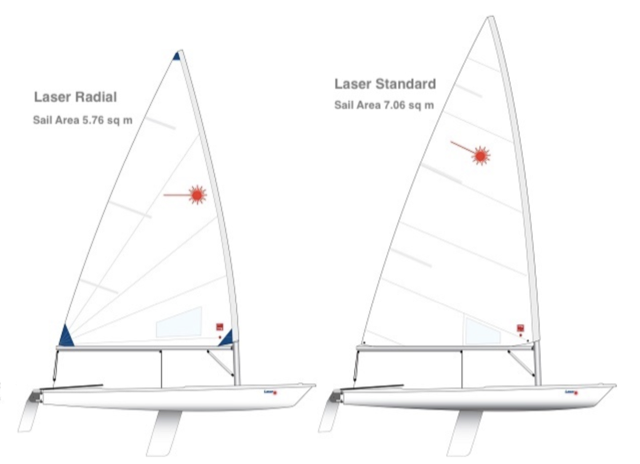
\includegraphics[width=0.65 \linewidth]{LaserOlympicClasses.png}
    \caption{Laser Olympic Classes. Laser standard refers to men category while Laser Radial is for women. The difference between them is only the size of the sail. \cite{2015LaserAssociation}}
    \label{fig:LaserSideView}
\end{figure}
The equations of section \ref{sec:eq_of_motion}, use the added mass over each axis which according to \cite{keuning2004mathematical} can be determined by equations \ref{eq:mx_add} and \ref{eq:my_add}. At this point, the \acrshort{crew_m} is required and for the purposes of this research, the maximum value suggested by \cite{laser_opt} is used. 
\begin{equation}\label{eq:mx_add}
    m_{x}=2\frac{T_{c}} {Loa} m_{T}=2\frac{T_{c}} {Loa} (m_{boat} + m_{c})=2\frac{0.787}{4.2}(59+70)=48.34 \text{ kg}
\end{equation}
\begin{equation} \label{eq:my_add}
    m_{y}=0.25 \cdot m_{T}=0.25 \cdot (59+70) = 32.25 \text{ kg}
\end{equation}
\par 
Most of the coefficients used on the equations of section \ref{sec:eq_of_motion} can be found on tables, however, they can be approximated by using sine and cosine functions \cite{rein2012tra},\cite{moreira2011guidance}. These coefficient approximations are referred to the keel ($C_{i,keel}$) and rudder ($C_{i,rudder}$) only and they are shown next, the sub-index \textit{L} is for the \textit{lift} while \textit{D} is for the \textit{drag}. \par 
\begin{subequations} \label{eq:keel_coeff}
    \begin{align}
        C_{L,keel}=0.615sin(2\beta_{k_{a}})+0.025 \label{eq:keel_Liftcoeff}\\ 
        C_{D,keel}=-0.55cos(2\beta_{k_{a}})+0.55 \label{eq:keel_Dragcoeff}
    \end{align}
\end{subequations}
\begin{subequations} \label{eq:rudder_coeff}
    \begin{align}
        C_{L,rudder}=0.6175sin(2\beta_{r_{a}})+0.0325 \label{eq:rudder_Liftcoeff}\\ 
        C_{D,rudder}=-0.55cos(2\beta_{r_{a}})+0.55 \label{eq:rudder_Dragcoeff}
    \end{align}
\end{subequations}
Due to these approximations equations \ref{eq:Side_force}, \ref{eq:att_r} and \ref{eq:att_k} are modified and facilitate the separation of the \textit{lift} and \textit{drag} forces to use them. The angle of attack (\acrshort{a_a})is related to the \acrshort{b_aw}, therefore it is associated with the trim angle of the sail (\acrshort{trim_sail}). The keel is a fixed element and it is assumed rigid then \acrshort{b_k_a} is the same as the \acrshort{b_ac}.   \par \noindent %The approximations related to the sail will not be used since equations \ref{eq:draftMod} and \ref{eq:liftMod} 
\begin{equation} \label{eq:app_current_ang}
    \beta_{ac}=atan2\frac{v}{u}
\end{equation}
\begin{equation} \label{eq:app_current_vel}
    V_{ac}=\sqrt{u^2 + v^2}=V_{boat}
\end{equation}
\begin{equation} \label{eq:keel_lift}
    F_{L,keel}=\frac{1}{2} \cdot \rho_{w} V_{ac}^2 A_{keel}C_{L,keel}(\beta_{ac})
\end{equation}
\begin{equation} \label{eq:keel_drag}
    F_{D,keel}=\frac{1}{2} \cdot \rho_{w} V_{ac}^2 A_{keel}C_{D,keel}(\beta_{ac})
\end{equation}
\begin{equation} \label{eq:angle_attack_rudder}
    \beta_{r_{a}} = \beta_{ac} - \delta_{r}
\end{equation}
\begin{equation} \label{eq:rudder_lift}
    F_{L,rudder}=\frac{1}{2} \cdot \rho_{w} V_{ac}^2 A_{rudder}C_{L,rudder}(\beta_{r_{a}})
\end{equation}
\begin{equation} \label{eq:rudder_drag}
    F_{D,rudder}=\frac{1}{2} \cdot \rho_{w} V_{ac}^2 A_{rudder}C_{D,rudder}(\beta_{r_{a}})
\end{equation}
\begin{equation} \label{eq:angle_attack_sail}
    \alpha_{a} = \beta_{aw} - \delta_{sail}
\end{equation}
The motion of the sailboat is dominated by the wind and this research is focused on the effects of the wind. As a result, the $\beta_{i_{a}}$ of the rudder and keel are treated as one component and substituted by $\alpha_{a}$ \cite{rein2012tra}. The implication of this substitution has two effects, first on the \acrshort{Rhull} and second on the lateral force. The coefficient related to the \acrshort{Rhull} has to account for thus it has to increase to \textit{0.025}. \textbf{The lateral forces are assumed to be in equilibrium all the time,  as a result, the \acrshort{v} velocity known as drift speed is neglected} hence equation \ref{v_dot} is omitted from the equations of motion for the Laser Class \cite{rein2012tra}.\par  
Another modification is identified with the equation \ref{eq:u_dot} which has to be modified to replace the hydrodynamic derivative expression ($X_{V\psi}$) by a damping expression showed on the equation \label{eq:u_dotLaser}. The damping expression is related to a constant value  (\textit{Cnst}) of 0.3 according to \cite{rein2012tra}. \par
\begin{equation} \label{eq:u_dotLaserM}
    \Dot{u}=\frac{X_{TOT}}{m+m_{x}}-Cnst \cdot \Dot{\psi}^2
\end{equation}
To recapitulate all the previous changes, the equations of motion that describe the motion for the Laser Olympic Class are: \par 
\begin{equation} \label{eq:X_uM}
    X_{U}=\frac{1}{2}\rho_{w}V_{boat}^2 \cdot C_{D,hull}=\frac{1}{2}\rho_{w} \cdot V_{ac}^2 \cdot 0.025 
\end{equation}
\begin{equation}\label{eq:X_sailM}
       X_{sail}=F_{L,s}sin\beta_{aw}-F_{D,s}cos\beta_{aw} 
\end{equation}
\begin{equation}\label{eq:Forces_M} 
     X_{current}=m\cdot V_{boat} \Dot{\psi}= m\cdot V_{tc}^b \cdot \Dot{\psi}
\end{equation}
\begin{equation}\label{eq:X_TOTM}
    X_{TOT}=X_{U}+X_{sail}+X_{current}
\end{equation}
where:
\begin{equation} \label{eq:SailLiftM}
    F_{L,s}=\frac{1}{2}\rho_{a}V_{aw}^2 \cdot A_{s} C_{t}^*
\end{equation}
\begin{equation} \label{eq:SailDragM}
    F_{D,s}=\frac{1}{2}\rho_{a}V_{aw}^2 \cdot A_{s} C_{d}^*
\end{equation}
Finally, the equations that describe the motion are:\par
\begin{equation}\label{eq:x_dotM}
\Dot{x}=u \cdot cos\phi + u_{tw} + u_{tc}
\end{equation}
\begin{equation}\label{eq:y_dotM}
\Dot{y}=u \cdot sin\phi + v_{tw} + v_{tc}
\end{equation}
\begin{equation} \label{eq:u_dotLaserMR}
    \Dot{u}=\frac{X_{TOT}}{m+m_{x}}- 0.3 \Dot{\psi}^2
\end{equation}

These modified equations serve only for the laser Olympic class and with them, the \acrshort{vpp} can be estimated. Even so, at some wind velocities the %the approximations of 
equation \ref{eq:liftMod} %and \ref{eq:keel_coeff}
could be less accurate, especially at \acrshort{v_tw} close to 20 kn and above it. Since equations \ref{eq:liftMod} and \ref{eq:draftMod} work fine when the \acrshort{v_tw} is close to 10 kn \cite{day2017performance}, which is at the lower range of the \acrshort{v_tw} range defined by \cite{laser_opt}. \par 

\subsection{ VPP for the Laser Olympic Class}
The optimization of the minimal time path as showed in equation \ref{eq:rabaudmintime} requires to determine first the velocity which in this case \acrshort{v_aw}($\psi$). \acrshort{v_aw}($\psi$) is related to the wind speed and direction and considering the computational effort and the fact that the wind model is space and time discretized. The \acrshort{vpp} can be estimated first since the wind speed range rule ([4,25]kn) conditions the laser races. To estimate the \acrshort{vpp} not only the \acrshort{b_tw} but also the \acrshort{v_boat} has to be discretized with small steps values. \par \noindent 
Using the previous equations and replaced in equations from \ref{eq:X_tot} to \ref{y_dot} the \acrshort{vpp} can be obtained using an optimization method. The systems of equations can be solved over the angle range of [0,180 \degree] using the built-in function of \textit{fmincon} from \acrshort{matlab}\cite{rein2012tra}. The problem is defined as maximization of the \acrshort{v_boat} which means that all the forces are in equilibrium. However, any  optimization problem has to be defined in terms of the minimum value, then the problem is defined as:
\begin{align}
    \text{minimize:}\qquad & -u(u,\psi,\delta_{s},V_{tw})  \label{eq:max}\\
\text{subject to:} \qquad & X_{TOT}=0 \\
 \qquad & Y_{TOT}=0
%& \Dot{v}=0 \\
%& \Dot{\psi}=0
\end{align} \label{eq:opt_vpp2}
instead of: 
\begin{align}
    \text{maximize:}\qquad & u(u,\psi,\delta_{s},V_{tw})  \label{eq:max2}\\
\text{subject to:} \qquad & \Dot{u}=0 \\
%& \Dot{v}=0 \\
& \Dot{\psi}=0
\end{align} \label{eq:opt_vpp}
Equation \ref{eq:max} shows that \acrshort{u} is the boat's velocity and it depends on itself which means that the system is not linear. Moreover, its influence on \acrshort{b_tw} \acrshort{v_aw} determines the sail's forces. The control variables this problem are $\Dot{\psi}$ and \acrshort{trim_sail}, this last could have a value over the range of [0,180 \degree] but it should not cancel $\Psi$, during motion.
\par
\begin{figure}[hbt!]
    \centering
    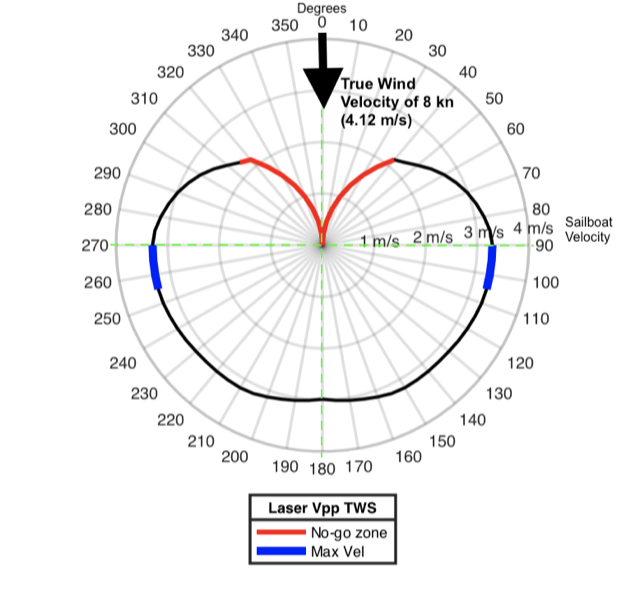
\includegraphics[width=.53 \linewidth]{Vpp_8.png}
    \caption{Full VPP for the Laser Class at 8 kn $V_{tw}$ coming at $0\degree$ from the North, the angles were discretized with an interval of $10\degree$} 
    \label{fig:Laser_Full_Vpp85}
\end{figure}
Figure \ref{fig:Laser_Full_Vpp85} shows the full \acrshort{vpp} of the Laser Olympic Class for a wind of 8 kn. In this graphic, the direction of the wind is zero degrees from the North. The angle's interval is $10\degree$ and the \acrshort{v_boat} is indicated by the diameter of the circles, in this case, it has a range value of [0,3.3] m$\backslash$s. In the figure, the \textit{no-go-zone} is in the angle range of [0, 40] degrees and [320, 360] degrees while the maximum velocity of the boat can be reach in the angle range of [90, 115] degrees and [255, 270] degrees. \par 
\noindent
The \acrshort{v_boat} range taking out the \textit{no-go-zone} is [2,3.3] m$\backslash$s, the \acrshort{vpp} shape over the range of [90,270] degrees does no vary too much. The shape is close to a semi-circle, this means that under a downwind condition a straight trajectory could be more efficient if the tack loss time is bigger than the velocity change ratio while the \acrshort{v_tw} remains are constant.  \par  

An alternative method to estimate half of the  \acrshort{vpp} uses wind measurements for the speed and its direction. These measurements, however, do not have a constant interval, so to predict any other wind speed and its direction, the measured data is interpolated  
%Interpolating between known values can then give predicted maximum speeds for any true wind angle and true wind speed
\cite{philpott2001optimising},\cite{allsopp2000optimal}. For the purpose of this project, some wind measurements for wind speed  were provided by \acrlong{sailctr}. \par \noindent 
The interpolation used for the missing points was the \acrfull{pchip} from \acrshort{matlab}. The use of this data not only serves as validation for the \acrshort{vpp} calculations but also as a data source. This because of many of the research regarding \acrshort{vpp} for the Laser Olympic Class only cover a wind speed range of [9,12] kn \cite{day2017performance} and the measurements provided are out of this range and they are shown in figure \ref{fig:hvpp_MeasData}.\par \noindent
Figure \ref{fig:hvpp_MeasData} indicates the measurements taken with a black asterisk, the rest of the points, therefore the line is the result of the \acrshort{pchip} interpolation. The wind measured is referred to as \textit{TWS} and it is assumed to come from the North, top of the graph. The \acrshort{vpp} is assumed to be symmetric and due to this, the measurements were only taken in the range of [0,180] degrees. \par 
\begin{figure} [hbt!]
    \centering
    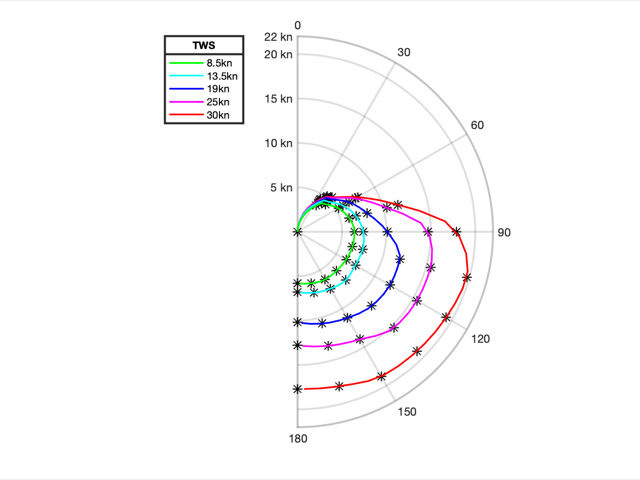
\includegraphics[width=0.72 \linewidth ]{Half_Vpp_laser2.png}
    \caption{Vpp developed with measurements provided by $InnoSportLab\textsuperscript {\textregistered}$, The Hague. The measurements are indicated with a black asterisk. The results of the interpolation vary according to the wind velocity (TWS)}
    \label{fig:hvpp_MeasData}
\end{figure}
The measured data not only serves to develop the \acrshort{vpp} but also to validate some of the assumptions previously made. Now that the \acrshort{vpp} was determined the formulation of the minimal time path for the Laser Sailing Class can be described.  \par 

\subsection{The Objective Function: The Minimal Time Path}
At this point, all the elements required to develop the algorithm have been explained. In this section, their implementation is going to take place. The objective is to find the path with the minimum time, regardless of the type of sailing course. Figure \ref{fig:SailModes_Man}, shows the three types of courses with its main maneuvers and an angle range where they take place. The angle range is not specified since it depends mainly on the \acrshort{vpp} (according to the sailboat) and sailor preferences. For example, under a downwind condition, many sailors prefer to follow a straight line rather than a zig-zag pattern.  \par
\begin{figure} [hbt!]
  \centering
  \subfloat[The 3 main modes to sail respect to the wind direction.]
  {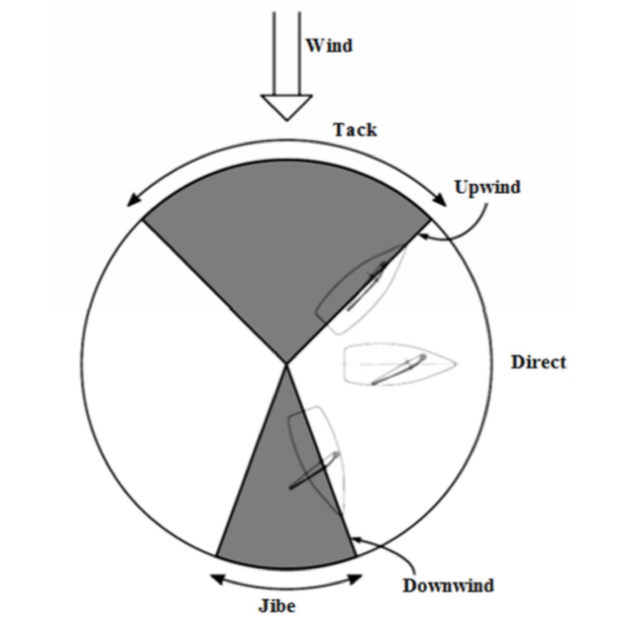
\includegraphics[width=0.45 \linewidth]
  {SailingModes.png}\label{fig:SailModes}}
  \hfill 
  \subfloat[Types of Maneuvers for sailing according to the boat and wind direction.]{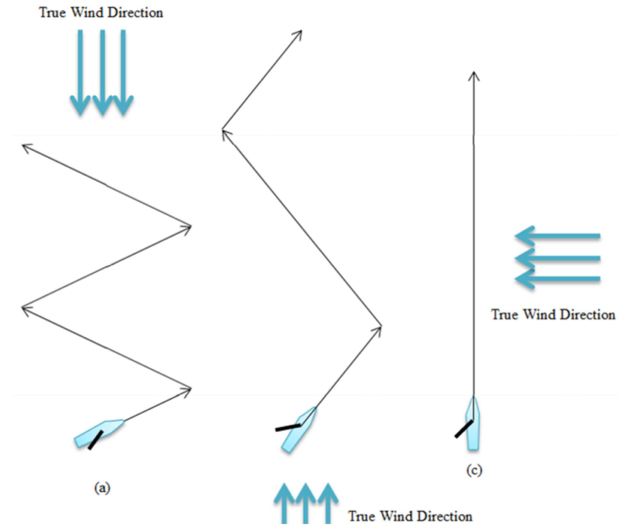
\includegraphics[width=0.5 \linewidth]
  {SailinMAnu.png} \label{fig:maneuversType}}
  \caption{Type of courses and its Maneuvers \cite{Alves2014ASailboat}}
\label{fig:SailModes_Man} 
\end{figure}

The combination of at least two of these sail-modes determines a race for Olympic Sailing Competitions. Each sail-mode over the course is defined as \textit{Leg}, them the minimal time for the race is given by the minimal time on each leg. This optimization problem is defined as a multi-phase problem, where each \textit{leg} is the phase of the problem. It is a multi-phase problem not because all the phases are connected but because on each phase different sets of constraints are implemented.\par
Each leg of the course to race is defined by the index \textit{i} and it starts at 1. %, the total number of legs on a race is 5 but this value could change.. 
The number of stages or states of the variables is defined by the index \textit{n} and it can be described as an intermediate set of points inside each \textit{i leg} where the time and distance are evaluated.  This means that if there are two legs in total and the number of stages is 5, therefore there are twelve stages in total (\textit{$n \times i = (5+ 1) \times 2 = 12$}).\par 
The approach of this problem is based on direction-dependence technique with the heading-angle decision to generate \textit{k} sub-routes. The reason for the \textit{k} sub-routes is to evaluate the symmetry of the \acrshort{vpp} especially at the beginning of the race.
This not only for the upwind mode and \textit{answer the question of why start to port is better (or not) than start to starboard}, furthermore to evaluate the straight-line trajectory over the rest of the wind modes. \par \noindent %on the downwind and direct(reach) mode
Consequently, \textit{k} is assigned to have \textit{three values}, 1 for the straight-line trajectory, 2 is for the port(left) and 3 is for the starboard (right) start direction. As a note, on the upwind condition, the straight-line is not evaluated, nor optimized. Further details about \textit{k} and \textit{n} are given oncoming sections of this chapter.\par 
Then the minimal time path for the Olympic Laser races is based on equation \ref{eq:rabaudmintime} and defined as follow.
The objective function is established by equation \ref{eq:minTO} and it is composed of two terms. The first term accounts for the accumulated minimal time up to the previous \textit{i leg} and it stores the  \textit{k,n} state-space variables of the previous legs, as established on equation \ref{eq:CollectPointsTime}.
The second term is the minimal time for the current \textit{i leg} from the \textit{k} sub-route over the \textit{n} stages. \par \noindent 
The time on the second term is determined by the velocity $v_{k,n}$ which depends on its heading-direction, and on the length's trajectory ($dl_{k,n}$). This means that $v_{k,n}$ is  conditioned by equations \ref{eq:C_xvel} and \ref{eq:C_yvel}, and estimated with equation \ref{eq:VelovertheLenght}.
\begin{align}
%\min_{j \in \Gamma_{i}}\\ 
    \text{min } & T=
    %\int_{t_{0}}^{t_{f}} dt=
    L_{k,n}^{i-1}(\Psi,t_{f})+ min \bigg[ \int_{t_{0}}^{t_{f}}  \frac{dl_{k,n}^i}{v_{k,n}^i} \bigg] \quad ,k \in \{1,2,3\} \label{eq:minTO}\\
\text{subject to:} \quad & \Dot{x}=u(\Psi)cos(\Psi) + u_{tw}+u_{tc} \label{eq:C_xvel} \\
\quad & \Dot{y}=u(\Psi)sin(\Psi) + v_{tw}+v_{tc} \label{eq:C_yvel}
\end{align}
where:
\begin{equation}\label{eq:CollectPointsTime}
     L_{k,n}^{*}(\Psi,t_{f})=[x_{k,n}, y_{k,n},t_{f}]^{*}
\end{equation}
\begin{equation}\label{eq:VelovertheLenght}
     v_{k,n}^{*}=\sqrt{\Dot{x}^2+\Dot{y}^2}
\end{equation}
The boundary conditions showed on equations \ref{eq:locIniX}, \ref{eq:locFinX}, \ref{eq:locIniY} and \ref{eq:locFinY} are determined by the leg, particularly by the location of the start buoy and end buoy. These buoys are located over the sailing area and they determine the direction of the boat to follow along with the direction of the wind, to arrive at the next buoy. The location of each buoy is provided in Cartesian coordinates, as explained in \ref{sec:RefFrames}, the latitude-longitude coordinates can be converted to [X,Y] using the \acrshort{matlab} function \textit{deg2utm(Lat,Lon)}. Equation \ref{eq:InitialTime} defines the initial time for the first leg (\textit{i=1}) which is zero. The initial time for the next leg is given by the final time of the previous leg, as shown in equation \ref{eq:FinalTimeLeg}.\par 
\begin{align}
    \quad & x_{k}(0)^i=x_{1}\label{eq:locIniX} \\
    \quad & x_{k}(t_{f})^i=x_{2}\label{eq:locFinX} \\
    \quad & y_{k}(0)^i=y_{1}\label{eq:locIniY} \\
    \quad & y_{k}(t_{f})^i=y_{2}\label{eq:locFinY}\\
    \quad & t_{0}^1=0 \label{eq:InitialTime} \\
    \quad & t_{0}^{i}= t_{f}^{i-1} \label{eq:FinalTimeLeg}
\end{align}
\par 
To connect all the legs, and predict the optimal time path for the whole race, the next equations \ref{eq:x_linkC} and \ref{eq:y_linkC}, gives continuity to the path. This continuity helps the algorithm to control the tacking maneuver and estimate the tack angle for each leg change.
\par 
\begin{align}
    \quad & x^{i+1}(t_{0}^{i+1})=x^{i}(t_{f}^{i})\label{eq:x_linkC}\\
    \quad & y^{i+1}(t_{0}^{i+1})=y^{i}(t_{f}^{i}) \label{eq:y_linkC}
\end{align}
\par 
The tack maneuver refers to the change in direction due to a change of a leg, in other words, it is a transition maneuver. This transition maneuver or the turn/tack angle is the angle between the end section (stage) of one leg with the start  section (stage) of the next leg and it is constrained by two equations showed as following and in figure \ref{fig:tackAngL}.\par
\noindent
for the tack to port:
\begin{equation}\label{eq:tackportC}
40\degree < \Psi_{n_{max}-1}^{i}(t_{f}^{i}) -
\Psi_{n+1}^{(i+1)}(t_{0}^{i}) < 130 \degree
\end{equation}
\noindent
and for the tack to starboard:
\begin{equation}\label{eq:tackstarbC}
-130\degree < \Psi_{n_{max}-1}^{i}(t_{f}^{i}) -
\Psi_{n+1}^{(i+1)}(t_{0}^{i}) < -40 \degree
\end{equation}
\begin{figure} [hbt!]
    \centering
    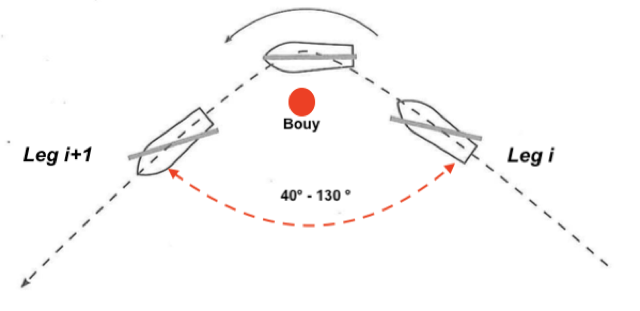
\includegraphics [width=0.55 \linewidth]{tack.png}
    \caption{Tack angle range between legs.}
    \label{fig:tackAngL}
\end{figure}
\par 
The final time on each leg is the minimal time and the result of the optimization over that \textit{i leg} and \textit{k} start direction. However, it is known that on the upwind condition, the Laser follows a zig-zag pattern to move against the wind. Moreover, each of these changes in direction takes time and speed and this has to quantify. For example, \cite{rein2012tra} mentioned a speed loss of 2 kn due to change in direction, other authors refer to these changes as a delay in time of about 4 to 10 seconds before they are reflected in the trajectory \cite{keuning2004mathematical}, \cite{Alves2014ASailboat}.\par \noindent % \hl{(\textbf{find reference from ch1 and ch2})}. \par \noindent
In this algorithm, the number of changes in the trajectory is quantified as a time loss added to the final time on each leg by equation \ref{eq:FinalTime}. The time loss to add of the equation \ref{eq:Tot_TimeLoss} depends on the total number of changes in direction during the \textit{i leg}, set on equation \ref{eq:shiftDirCount}, multiply by a constant defined as a $t_{tack-loss}$ and its value is defined in further sections on this chapter. In addition, the equation \ref{eq:shift_Dir} controls these shifts in the direction so changes larger than 180 \degree  does not happen.\par 
\begin{equation}\label{eq:shift_Dir}
    0 \degree <=\Psi_{k,n+1}^{i}(t_{f}^{i}) - \Psi_{k,n}^{i}(t_{0}^{i}) <180 \degree
\end{equation}
\begin{equation} \label{eq:FinalTime}
e\end{equation}
\begin{equation} \label{eq:Tot_TimeLoss}
    \Delta T_{loss}^i=t_{tack-loss} \sum_{n=1}^{n} \Delta \Psi_{k}^* (i)
\end{equation}
\begin{equation} \label{eq:shiftDirCount}
\Delta\Psi_{k}^*(i)=
\begin{cases}
0, \quad  \text{if: } \Psi_{k,n+1}^{i}(t_{f}^{i}) = \Psi_{k,n}^{i}(t_{0}^{i})\\
\\
1 %\quad  \text{if: } \Psi_{k,n+1}^{i}(t_{f}^{i}) \neq  \Psi_{k,n}^{i}(t_{0}^{i})\\
\end{cases}
\end{equation}
\begin{equation} \label{eq:TimeFinal_acum}
    t_{f}^{*i}=\sum_{i=1,k}^{i} \Big( t_{f}^{i,k} - t_{0}^{i,k} \Big)
\end{equation}
The state-space limits for the variables are defined in equation \ref{eq:xlox_leg_alt}, \ref{eq:ylox_leg_alt} and \ref{eq:Dirlox_leg_alt}.  The first two limits the position of the sailboat while the last limits the heading angle ($\Psi$) to evades the \textit{no-go-zone}.
\begin{align}
    \quad & x_{min}^{i,1}<x(t)_{n}^{i,1}<x_{max}^{i,1} \label{eq:xlox_leg_alt}\\
   \quad & y_{min}^{i,1}<y(t)_{n}^{i,1}<y_{max}^{i,1} \label{eq:ylox_leg_alt}\\
   \quad & \Psi_{min} <\Psi(t)< \Psi_{max} \label{eq:Dirlox_leg_alt} \\
  \text{where:} \quad & 40\degree  <\Psi(t)< 320\degree \nonumber 
\end{align}
 As mentioned before on each leg the state-space constraints are different, to determine these limits the coordinates of the midpoint of the straight-line trajectory (\textit{k=1}) between buoys are required. The tolerance factor $x_{SAtot}$ and $y_{SAtot}$ determine the minimum and maximum values of the coordinates and defined the limits on each leg. The next equation shows how these estimations are done. In the case of the minimum value or lower bound, it requires the minimum coordinate for \textit{X} and \textit{Y} coordinates from the \textit{3 sub-routes} while for the upper limit, it is the maximum of them, in both cases, it is also required the $x_{mean}^{i}$ \textit{mean values from the 3 sub-routes (k)}. \par 
 
 The value of this factor should be chosen carefully, one of the reason is that a bigger area not always have more nodes, and the algorithm will take more time to estimate the optimal solution. Moreover, it is possible that a local minimum will be found instead of the global solution, because of this it was suggested to run the algorithm several times guessing some of the initial conditions. The next iterations serve to tune these conditions until they remain the same \cite{philpott1993yacht}. %and changing them for the next time. If the solution remains the same the solution is the optimal, otherwise  
\begin{equation} \label{eq:Xmin_SailArea}
    x_{min}^{i}=x_{mean}^{i} - x_{SAtol}\cdot \Biggm|  x_{mean}^{i} -  min \bigg( x(t_{0}^{i})^{i},x(t_{f}^{i})^{i} \bigg) \Biggm| 
\end{equation}
\begin{equation} \label{eq:Xmax_SailArea}
    x_{max}^{i}=x_{mean}^{i} + x_{SAtol}\cdot  \Biggm|  x_{mean}^{i} -  max \bigg( x(t_{0}^{i})^{i},x(t_{f}^{i})^{i} \bigg)  \Biggm| 
\end{equation}
\begin{equation} \label{eq:Ymin_SailArea}
    y_{min}^{i}=y_{mean}^{i} - y_{SAtol}\cdot \Biggm|  y_{mean}^{i} -  min \bigg( y(t_{0}^{i})^{i},y(t_{f}^{i})^{i} \bigg) \Biggm| 
\end{equation}
\begin{equation} \label{eq:Ymax_SailArea}
    y_{max}^{i} = y_{mean}^{i} + y_{SAtol}\cdot \Biggm|  y_{mean}^{i} -  max \bigg( y(t_{0}^{i})^{i},y(t_{f}^{i})^{i} \bigg) \Biggm| 
\end{equation}

The optimization problem and its constraints for the minimal time path for the Laser Class have been defined. These constraints not only helps the algorithm to get the optimal solution but also to connect all the legs. The connection between legs is made by means of the tack angle, a simplify approach followed for the purposes of this research \cite{jouffroy2009steering}, \cite{LinXiao2011ModelingYachts}.\par 
The state-space constraints are coupled not only with the wind forecast model but with the course of the competition. Even when some space boundaries varies according to the leg to course, it is the orientation of leg relative to the wind angle the parameter that tunes the boundaries of this area. For this reason, a further section will explain how the integration of the curse is made, more precisely the locations of the buoys into the minimal time path trajectory.\par 

% which is simplification approach to acknowledge.    For more details review 
 \subsection{Definition of the Sub-routes (\textit{k=2,3}) at the port and starboard direction} \label{sec:sub_routes_DEF}

The optimization algorithm initializes using one of the 3 alternative sub-routes and they are identified by the \textit{k} index. %these sub-routes are set up in the same way as any leg. 
The reason for them is not only because of the heading-angle approach but also because of the \textit{fmincon} function from \acrshort{matlab} request initial values of the variables used on the cost function to find the optimal solution. Because the problem is non-linear, this means that starting at different points could get different results and these different start conditions facilitate the algorithm to converge to the optimal solution %the problem by starting at different points 
\cite{mitchell2000geometric}, \cite{kelly2015transcription}. \par 

Starting at different points allows the conversion of the solution, however, in this case, it also aim to the strategy of the race for coaches and athletes. In addition, it aims to limit the area within the optimal path is found and reduces the computational effort also. Because the \acrshort{vpp} has a non-convex shape a path attainable region can be defined, the implication of a non-convex \acrshort{vpp} implies that the optimal path may not be unique \cite{dolinskaya2012time},\cite{dolinskaya2013fastest}.  For example, on the upwind condition, the maximum velocity is found after the 40\degree, and there are two possible trajectories to follow and reach the next buoy using also the \acrshort{vmg} criterion. \par 
First, at 45\degree the sinus and cosine functions have the same value and it is out of the \textit{no-go-zone}. This means that it is possible to sail at 45\degree respect to the wind direction until the midpoint %on the \textit{X-coordinate} 
and then tack at -45\degree until the target buoy is reached. By doing these tacking maneuvers on both directions port and starboard directions, the sailing area for each leg can be set up. This area can also be stretched using the $x_{SAtol}$ and $y_{SAtol}$, this is done to give additional space for possible wind shifts, \cite{xing2012path}. \par \noindent
The second alternative is to tack at 45\degree until the target buoy can be reached by making a turn of 90\degree respect to the wind. This alternative was not followed, first because even when the velocity at 90 \degree is the fastest the distance to sail is the larger. Moreover, under a constant wind speed and  direction, the ratio between the distance to sail versus the ration between velocities is larger. Therefore, there is no advantage to sail at a higher velocity because the distance to cover does no compensate the increment on the velocity and this only increase the time to reach the target buoy. \par 
\begin{figure}[hbt!]
    \centering
    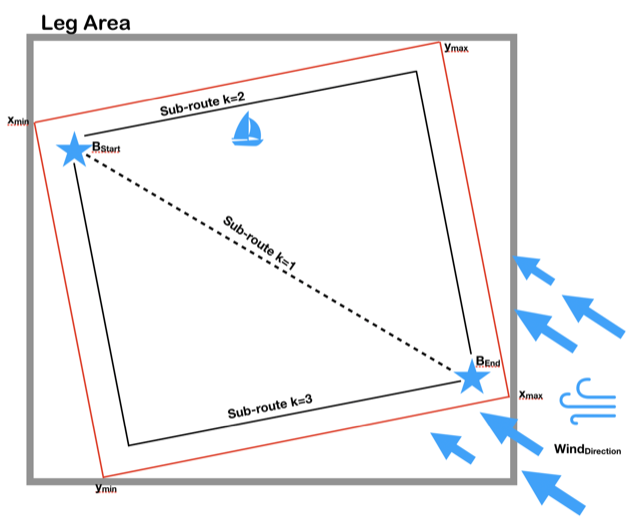
\includegraphics[width=0.5 \linewidth]{LegSail.png}
    \caption{Example of a Sail Area for a Leg using the sub-routes}
    \label{fig:LegSailArea}
\end{figure}
Following the first alternative 2 sub-routes where developed one for the port direction which is assigned by \textit{k=2} and the other to starboard assigned by \textit{k=3}. For the rest of the wind conditions, the same approach is followed to define these two sub-routes and therefore the bounds for the sailing area on each leg.  \par
The \textit{n} stages of each sub-route are located within each sub-route, so \textit{n} are points defined by \textit{[X,Y]} coordinates and its location determines the path to follow for a particular leg. In addition to this \textit{n} stages, a number of intervals between them were defined to describe properly the $dl_{k,n}^{i}$ of the objective function (equation \ref{eq:minTO}).  This number of intervals and the \textit{n} stages are designated at the beginning of the algorithm and they are part of the initialization parameters a large number for the interval value is recommended to have a smooth path, so the interval is designed by equation \ref{eq:interval}. For example, \textit{9 stages} with \textit{100 intervals} it generates \textit{1010} length elements per sub-route. \par 

\begin{equation} \label{eq:interval}
   \text{Interval: }  m=100
\end{equation}
\begin{equation} \label{eq:interval-example}
  elements_{dl}=(n+1) \cdot (m+1)
\end{equation}

These sub-routes serves to define the limits on each leg, not by the means of coordinates of each point but by the maximum and minimum value of those coordinates. The shape of the area for each leg is a rectangle where the coordinates of the opposite corners are defined as equations \ref{eq:Xmin_SailArea}, \ref{eq:Xmax_SailArea}, \ref{eq:Ymin_SailArea} and \ref{eq:Ymax_SailArea} an example of this area is showed in figure \ref{fig:LegSailArea}. In later sections, it will be clear that this sub-routes not only facilitates the algorithm in terms of the space constraints but also in finding the optimal solution for each leg. \par 
%Because inside each leg numer of \textit{n} st
%The algorithm is build in states (\textit{n}) inside each leg \textit{n}) , along each stage the dl will take place. The reason of this is to control the number of tacks along the leg, and in such way the zig-zag could be define.

\subsection{Course Integration into the Time Optimization Path Algorithm} \label{sec:Coure_LegIntegration}

The setup of the course is defined by the organizers of the event and this is done with the diagram and the location of the buoys using \textit{latitude-longitude coordinates}. The importance of them is because the space constraints explained before are linked with the legs of the course which in consequence are related to the buoy's location. The location of the buoys define the distance to sail, the angle direction of the leg respect to the wind direction and as a result, the wind mode to sail. \par 

An example of the information about the course is showed in figure \ref{fig:Rio_Course1} and it shows a \textit{trapezoid course}, where the start and end of the competitions are defined by a line. In this course, there are 6 buoys, 2 line indicator and 2 boats. The letter next to the number of the buoy indicates it locations respect to the boat, so \textit{s} is for \textit{starboard} and \textit{p} for \textit{port}. The order of the marks, indicated in the table below of the diagram, describes how the legs are designated and the code or signal for that sequence. The coordinates of the buoys are provided previously to the race since they depend on the wind direction and other factors.  \par 
\begin{figure} [hbt!]
    \centering
    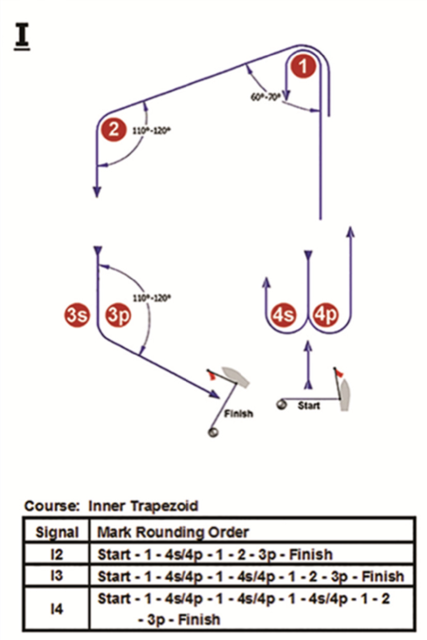
\includegraphics[width=0.41 \linewidth]{course_rio.png}
    \caption{The I Trapezoid Course diagram provided for the Sailing competitions on Rio 2016 Olympics \cite{sailoly}.}
    \label{fig:Rio_Course1}
\end{figure}
For the purposes of this research, the marks where a line is defined or where 2 buoys are designated with the same number, a midpoint is going to be calculated to represent this condition. However, for the start and the end line, the location of both ends is considered and the midpoint is also going to be calculated. The reason of these three points, on the start and on the end line is to account the variation of the wind direction and review how sensible is the time path on the first leg and on the last leg. \par

The location of the buoys most of the time is provided in \textit{latitude-longitude coordinates} and the units are degrees-minutes-seconds before to convert them to \textit{[X,Y] coordinates} they need to be converted to degrees. This conversion is made using the \textit{dms2degrees} from \acrshort{matlab}. Once this conversion is done and using the order of the buoys the algorithm will estimate the distance between them with the \acrshort{matlab} function \textit{pdist($b_{1},b_{2}$,'euclidean')}. \par \noindent The angle between them is based on the normal plane, since the wind angle respect to the \textit{North} is determined in degrees by equation \ref{eq:bouy_angle}, where \textit{i} is the index related to the leg. However, even when this expression only refers to the leg, it can be used to estimate the heading-angle($\Psi$) and  therefore $dl_{k,n}^{i}$. \par 

\begin{equation} \label{eq:bouy_angle}
    \theta_{{i}}=atan2d \bigg [\frac{x_{2}-x_{1}}{y_{2}-y_{1}} \bigg] ^{i}
\end{equation}

The wind mode of the leg is given by the difference between %the angle of the leg 
\acrshort{ang_bouy} %respect to the wind and
and the wind angle, %for now on it is defined as \textit{\acrshort{twd}} instead of 
\acrshort{b_tw}, depending on the difference between those angles the wind mode and its angle are defined by equation \ref{eq:wind_modesDef}. The wind mode angle of the leg (\acrshort{angLegWind}) is defined at the beginning of the competition (\textit{$t_{0}$}), in order to start the calculations of the sub-routes. In this case, %The \acrshort{twd} 
the \acrshort{b_tw} only depends on time in the next section is going to be explained how this value is determined since in section \ref{sec:SailinArea_WindModel} it was explained that it depends on 4 dimensions.\par 
\begin{equation} \label{eq:wind_modesDef}
\Omega_{i,t_{0}} = \mid \theta_{i}-\textrm{TWD}_{t} \mid,
- \quad 
    \begin{cases}
        \text{Upwind(Upw)} \quad &
            \begin{cases}
                0\degree  &\leq  \mid \theta_{i}-\textrm{TWD}_{t} \mid    \leq    45\degree \\
                315\degree  &\leq    \mid \theta_{i}-\textrm{TWD}_{t} \mid  \leq   360\degree \\
            \end{cases} \\ 
    \\
        \text{Direct(Rch)}\quad &
            \begin{cases}
                45\degree   &<     \mid \theta_{i}-\textrm{TWD}_{t} \mid \leq   135\degree \\
                225\degree &\leq \mid \theta_{i}-\textrm{TWD}_{t} \mid <  315\degree \\
            \end{cases}\\
    \\
        \text{Downwind(Dwn)}\quad &
            \begin{cases}
                135\degree &<  \mid \theta_{i}-\textrm{TWD}_{t} \mid <  225\degree \\
            \end{cases}
            
    \end{cases}\\
\end{equation}
The buoys and its orientations respect to the wind define the legs and the limits of the area for each leg using the sub-routes as a reference. The \acrfull{angLegWind} determines the maximum velocity that the sailboat can achieve, once the intensity and location of the boat are known.  Now that the parameters for the course on each leg are defined, the next section will be explained how the wind model is going to be integrated into the algorithm. \par 

\subsection{Coupling the Wind Model with the Sail Course} \label{sec:SailinArea_WindModel} %for the Time Optimization Path Algorithm
Until now, the optimization algorithm has been described along with the state-space constraints only in terms of spatial coordinates. In the other hand, section \ref{sec:WRF_WindM} has described the \acrshort{wrf} wind model in general, while section \ref{sec:WRF_WindM_FR} provides all the details for the model used on this research. To move the sailboat not only it needs a target but also to know the wind velocity \acrshort{v_tw} at a specific time and location.\par \noindent %where is going to be head sailboat from one point to another it the
This section describes how the wind model of section \ref{sec:WRF_WindM_FR} is integrated into this algorithm, so equation \ref{eq:VelovertheLenght} can be determined. The reasons for this integration and adaptation, first, is because the area covered by the \acrshort{wrf} wind model of section \ref{sec:WRF_WindM_FR} is much larger than the area of the course. Second, the time step ($\Delta t$) is about 10 minutes, meaning that the wind characteristics remain constant along this $\Delta t$. However, it is most probably that the space-time dimensions for the estimation of the \acrshort{v_tw} do not correspond exactly with the space-time coordinates of the grid from the \acrshort{wrf} model despite this its value has to be estimated. \par \noindent 
Moreover, the time at which the competition starts has to be included during the initialization of the algorithm in addition to the duration of the race and some delays, all these factors are considered for the definition of the \textit{time window}.\par

Previous to the race date, the location of the sailing course and the estimated time to start it are known. If the conditions are not meet the race could be a delay until this they are meet or in the worst case scenario, the race could be canceled. Because of this, using the start time and the duration of the race (estimated to be about \textit{one hour}). The \textit{time window} is estimated by equations \ref{eq:time_window0} and \ref{eq:time_windowf} adding a bonus time or tolerance up to \textit{three hours} for the upper limit and subtracting \textit{two hours} for the lower limit.\par

\begin{align} %
    \textrm{Time window} &=\big[\textrm{Time window}_{0},  \textrm{Time window}_{f} \big]\label{eq:time_window}\\
    \textrm{Time window}_{0}&=\textrm{Time start}_{floor}-\textrm{Lower Tolerance} \label{eq:time_window0}\\
    \textrm{Time window}_{f}&=\textrm{Time start}_{ceil}+\textrm{Upper Tolerance}+\textrm{Duration}_{Race} \label{eq:time_windowf}
\end{align}
\par
The tolerances are not the same for both limits because due to the weather conditions most of the time the competition could delay rather than changed for an earlier time. In cases where the time is not defined in hours only, the start time is rounded to a \textit{floor} value, while for the end time it is rounded to a \textit{ceiling} value. The round or floor value, in this case, is set for an integer hour value, but it can be changed for a half-hour or any other value. For example, if the start time is 13:25 hrs, the time window is:\par
\begin{align} %\label{eq:time_window}
   \begin{split}
        \textrm{Time window}_{0}&= 13:25\textrm{ hr}_{floor} -\textrm{2 hr}\\ 
        &= 13:00\textrm{ hr} - 2\textrm{ hr}
   \end{split} \label{eq:time_window0Ex}\\
    \begin{split}
        \textrm{Time window}_{f}&=13:25\textrm{ hr}_{ceil}+\textrm{3 hr}+\textrm{1 hr}\\
        &= 14:00 \textrm{ hr} + 3\textrm{ hr} +1 \textrm{ hr} \label{eq:time_windowfEx}
    \end{split}
    \\
    \textrm{Time window} &= \big[11:00,18:00 \big]
\end{align}
\par
The definition of the \textit{time window} helps to reduce the length of the \textit{time dimension} from the \acrshort{wrf} wind model. For example, in section  \ref{sec:WRF_WindM_FR} it was mentioned the size of their dimensions, which are (\textit{x,y,z,t}) 198 $\times$ 301 $\times$ 50 $\times$ 145, since $\Delta t = 10$ minutes. Using the previous example of the \textit{time window}, this means that instead of using the 145 time-datasets only \textit{43} time-datasets are used on this algorithm. This reduces the time of processing for this model since only approx. $30\%$ of them are used to determine the solution of the minimal time path.\par 

Previous to the competitions, with a couple of months in advance, the location and diameter of the course area are communicated to the participants. Using this information, without any details about the location of the buoys, the area from the wind model for this algorithm is defined as a circle inscribed in a square. The coordinates of the opposite corners of this square are modified as equations \ref{eq:Xmin_WindArea},\ref{eq:Xmax_WindArea},\ref{eq:Ymin_WindArea} and \ref{eq:Ymax_WindArea} indicate. The tolerance of the wind area is determined by the radius of the sailing course multiplied by \textit{$n_{sc}$} times the grid space  ($\Delta x$) of the \acrshort{wrf} wind model. \par
\begin{equation} \label{eq:Xmin_WindArea}
    X_{W,min}= X_{CTR,course}-\frac{\clock_{course}}{2} \cdot n_{sc}   \Delta x
\end{equation}
\begin{equation} \label{eq:Xmax_WindArea}
    X_{W,max}= X_{CTR,course} + \frac{\clock_{course}}{2} \cdot n_{sc}  \Delta x
\end{equation}
\begin{equation} \label{eq:Ymin_WindArea}
    Y_{W,min}= Y_{CTR,course}-\frac{\clock_{course}}{2} \cdot n_{sc}    \Delta x
\end{equation}
\begin{equation} \label{eq:Ymax_WindArea}
    Y_{W,max}= Y_{CTR,course} + \frac{\clock_{course}}{2} \cdot  n_{sc}  \Delta x
\end{equation}
\par
The value of \textit{$n_{sc}$} depends on the size of the grid, $\Delta x $, respect to the \textit{radius} of the course as indicated in equation \ref{eq:n_windTolerance}. Since the  \cite{race_pol2017} establishes that the trapezoid course must be contained in this area, so \textit{$n_{sc}$} is the next integer value from the ratio between them. If the coordinates of the buoys are known, the minimum and maximum value of all of them are used instead of the coordinates of the center of the sail area to define the corners of the wind area. \par % and the limits for the wind model are defined in a similar way. \par 
%\begin{equation}\label{eq:WRF_windArea}
%\end{equation}
\begin{equation} \label{eq:n_windTolerance}
    n_{sc}=\lceil \frac{\clock_{course}}{2 \cdot \Delta x}
\end{equation}
%\begin{equation} \label{eq:TolWindArea}
%2\cdot \Delta x =
%\begin{cases}
%\Delta x \textrm{,} \quad & \Delta x < 1000\\
%\Delta x\textrm{,} \quad & \Delta x 
%\end{cases}
%\end{equation}
\par 
Using the previous equation the wind area is defined for this algorithm and it is larger than the area of the course, figure \ref{fig:WindAreaSketch} sketch this concept. It shows that if the center of the sail area is sufficiently far for any grid data-point, for example, within a sail of area with a $\clock = 3 \Delta x$ it only contains \textit{four} data-points while within the wind area defined with the previous equations it contains 64 data-points.\par

It is important that regardless of the location or time, the algorithm should be capable to estimate the wind's velocity. % at any time and location. 
Particularly when the coordinates are not coincident with those of the grid from the wind model. Thus to estimate the velocity at any point over the space and time an interpolation method is required. The data-points around the point of interest must be enough to estimate this value, moreover the area defined for the wind.  \par 
%For example, %if the location is close to the limits of the sail area, the available datapoints are sufficient and the interpolation can be made without compromising 

\begin{figure} [hbt!]
    \centering
    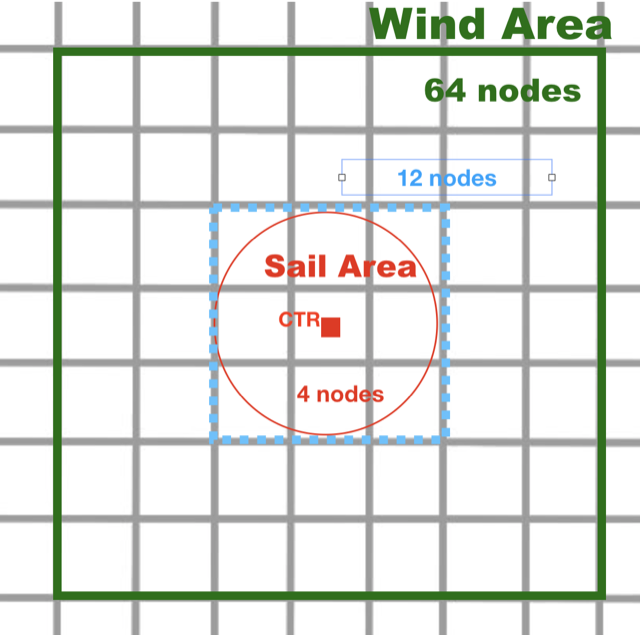
\includegraphics[width=0.32 \linewidth ]{gridWind.png}
    \caption{Wind Area Concept using a wind model representation. The inscribed sail area shows the limits of the square and its corners are used for the definition of the wind area.}
    \label{fig:WindAreaSketch}
\end{figure}

The interpolation method used in this algorithm is the \textit{griddata} function from \acrshort{matlab}. This function-method estimate the components of the wind's velocity %($u_{tw}$ and $v_{tw}$) at any time and position 
using the coordinates from the grid arrangement of the \acrshort{wrf} wind model. Figure \ref{fig:gridDataInterpo} shows a graphical representation of how this function and the wind model interact. It shows how two datasets for the velocity with coordinates \textit{[X,Y,t]} are used to determine the velocity $V_{tw}^{*}$ at $t^{*}$ which is intermediate from $t_{0}$ and $t_{1}$. Inside the function to obtain the requested value, a method has to be defined in cases where a linear interpolation doesn't apply. %for the interpolation of the values 
For the velocities, in this research, the \textit{nearest} option for the method is used inside the \textit{griddata} function.\par

\begin{figure}[hbt!]
    \centering
    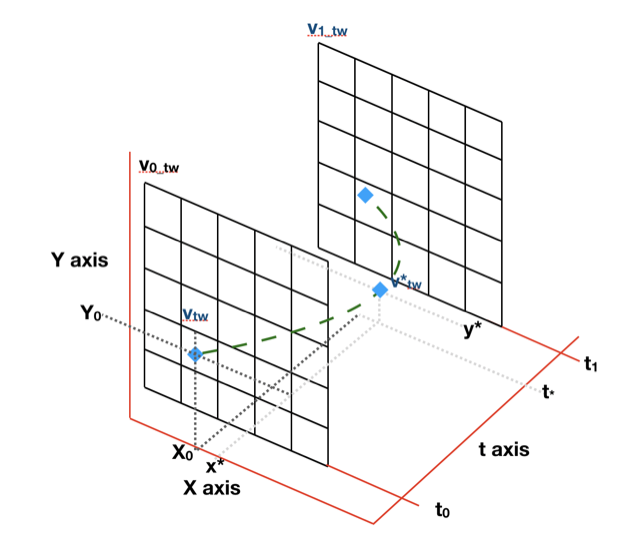
\includegraphics[width=0.47 \linewidth]{gridDataInterp.png}
    \caption{Griddata Method, a graphical representation of two datasets. The function interpolates the coordinates and values from the grid to obtain an intermediate value}
    \label{fig:gridDataInterpo}
\end{figure}

The coordinates used along this algorithm are \textit{[X,Y,t]}, this means that any data using \textit{[Lat, Lon]} coordinates have to be converted to \textit{Cartesian coordinates} (\textit{[X,Y]}), such as the buoys coordinates. In the case of the time dimension (\textit{t}), the units of the time step are defined in minutes, and this has to be converted to seconds, moreover, the number of digits after the point is only one. \par

The minimal time path algorithm not only requires the characteristics of the boat and athlete to solve the problem, but also constraints. These constraints are related to the state-space variables and they embody the environment within the competition takes place. In addition, to the type of maneuvers commonly used by athletes and sailor to sail from one point to another. But to represent properly the environment the area to sail has to be coupled to the wind area so the minimal time path can get a solution. \par \noindent 
Now that the algorithm has been defined and most of their parameter also, the next section will validate them. At the same, it will review that the parameters defined such as the number of stages is acceptable. All these to verify that a path developed using this algorithm represent the typical path of the laser class developed during races. \par % to meet the purposes of this research. 
%nm 1852 m
%2nm diamter
\section{Validation of the Algorithm: Results and Considerations}
\label{sec:ValidationAlgo}

The purpose of this section is to verify and validate the functionality of this algorithm to estimate the time of the predicted paths, thus to determine the minimal time path. These paths have to meet the constraints previous established and at the same time evaluate the values for the parameters assigned. Particularly the parameter for the number of stages per leg (\textit{n}) when the wind mode to sail is \textit{upwind}. In addition, to the constant related to the tack loss time ($t_{tack-loss}$) added to each of the shifts on directions of the laser class. By the end of the section, the considerations, and adjustments on the model required are mentioned in order to solve the optimization problem.  \par 

The validation is made on an upwind mode because during this mode the laser class is prone to follow a zig-zag pattern. As a result of this, it was defined that the wind speed (\acrshort{v_tw}) and direction (\acrshort{b_tw}) to be constant over time and space. In the other hand, the number of stages to evaluate begins at one (\textit{(n=1)}), so one shift in direction is made to reach the target.%at least one tack maneuver can be made.
\par 
The setup of the parameters and conditions represent the most simplified conditions to evaluate the algorithm but it can reveal easily if the algorithm works properly or not. The first aspect to review is that the algorithm identifies the \textit{no-go-zone}, for this the distance between marks is \textit{0.96 nm} equivalent to 1730 meters and $\Delta \Psi$ is 5\degree. Using these parameters, figure \ref{fig:Onestages_NoGoZone} shows that the algorithm develops more than. 346,000 nodes over the whole area defined inside a rectangle of approx. 8000$\times 4000 m$; however, many of these points are located above the target's location. The marks on green, only at one side of the start point are the nodes that meet the criteria about the angle and the \textit{no-go-zone}. The other side was not plotted %in this way to avoid confusion 
since the \acrshort{vpp} is assumed symmetrical.\par 

\begin{figure} [hbt!]
    \centering
    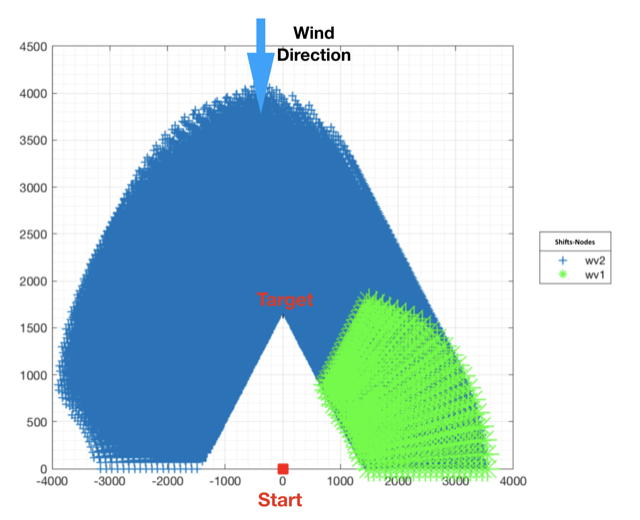
\includegraphics[width=0.45 \linewidth]{images/Nodes_2wv_5deg_5s.png}
    \caption{Nodes generated between 2 marks with one stage \textit{(n=1)} and  $\Delta \Psi = 5 \degree$}
    \label{fig:Onestages_NoGoZone}
\end{figure}

The values for the parameters and conditions to validate the algorithm are shown below. In this case, only half of the angles from the \acrshort{vpp}([0,$\pi$]) was used since it is assumed that it is symmetrical. Moreover, it is assumed constant wind conditions so the paths on both sides from the vertical line on the start mark are symmetrical. These parameters are:
\begin{itemize}
    \item \acrshort{v_tw}= 8.5 kn equivalent to 4.37 $ m/s $.
    \item \acrshort{b_tw}= 0\degree  from \textit{North}. 
    \item The distance between the start line and the next mark is \textit{0.977 nm} equivalent to 1809 meters. %\textit{0.96 nm} equivalent to 1730 meters. %1852 meters.
    \item The number of points stages is two, \textit{(n=2)}.
    \item The time step ($\Delta t$) is 5 seconds.
    \item The heading step angle ($\Delta \Psi$) is 1\degree. %5\degree.
    \item The $t_{tack-loss}$ = 10 seconds.
    \item The tolerance factor for the leg area are for $x_{SAtol}=2.5$ and for $y_{SAtol}=2$.
\end{itemize}

%For the next trial, $\Delta \Psi$ parameter was changed from 5\degree  to 1\degree, and the distance between marks was increased to \textit{0.977 nm} equivalent to 1809 meters, the rest of the parameter remains the same and only one side of the \acrshort{vpp} .
Under these conditions, more nodes were generated compared with figure \ref{fig:Onestages_NoGoZone}, and in consequence more paths with even the same time. This is shown in figure \ref{fig:Paths_2wv_1deg_5s} where paths inside the same time range were plotted with the same color. The figure also shows that the fastest paths do not shift after 1200 meter from the start point. In fact, figure \ref{fig:PathsTops_2wv_1deg_5s} shows that the paths with the top 5 times shifts before a horizontal distance of 1000 meters, which is only 10.5\% more than the midpoint distance between the marks. Despite the number of paths and its times the target mark hasn't reach perfectly 
%In this case with a smaller $\Delta \Psi$ and a larger distance between marks the paths never reach the target,
this is shown in figure \ref{fig:PathsZoom_2wv_1deg_5s}, where the second best time is the closets path within a radius of 6 meters from the target mark. % and it is the second best time that has this condition. \par
\begin{figure} [hbt!]
  \centering
  \subfloat[Paths generated with \textit{n=1} and $\Delta \Psi =1\degree$.] {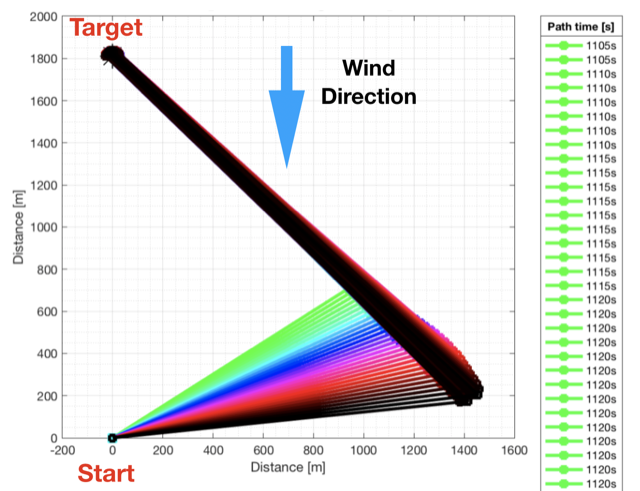
\includegraphics[width=0.31 \linewidth] {images/Paths_2wv_1deg_5s.png} \label{fig:Paths_2wv_1deg_5s}}
  \hfill
  \subfloat[Top 5 time paths and closets to the marked. These paths have the same time.] {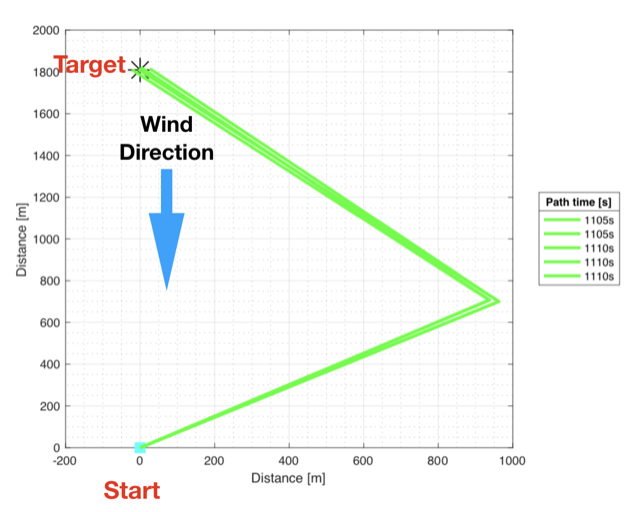
\includegraphics[width=0.31\linewidth]{images/PathsTop_2wv_1deg_5s.png}\label{fig:PathsTops_2wv_1deg_5s}}
  \hfill 
  \subfloat[Minimal time paths close-in end at the target mark.] {\includegraphics[width=0.31\linewidth] {images/ZoomPaths_2wv_1deg_5s.png} \label{fig:PathsZoom_2wv_1deg_5s}}
  \caption{Paths generated with one shift point in the direction (\textit{n=1}) and $\Delta \Psi =1\degree$.}
\label{fig:Nodes_Paths_2wv_1deg_5s}
\end{figure}

When the number of points-stages increase to two (\textit{n=2}), not only the number of nodes and paths increase but the top 5 times also increase by 5 seconds. In this case, the first shift in direction occurs at a horizontal distance from the start mark of 1100 meters and following the same heading-angle, figure \ref{fig:Path_3wv_1deg_5s}. The second shift on direction occurs within a radius of 46 meters from the target mark as shown in figure \ref{fig:PathZoom_3wv_1deg_5s}. But despite all these alternatives, the end of each of the paths does not reach perfectly the target mark. Figure \ref{fig:PathTops_3wv_1deg_5s} shows that all the paths with the same time end within a radius of 3 meters from the target mark.  \par 

\begin{figure} [hbt!]
  \centering
  \subfloat[Top 5 times using 2 attacks with $\Delta t$ =5s and $\Delta \Psi =1\degree$. The time for all the paths is 1100s] {\includegraphics[width=0.31 \linewidth]{images/Paths_3wv_1deg_5s.png} \label{fig:Path_3wv_1deg_5s}}
  \hfill
  \subfloat[Close-up of the top 5 times at the target mark. The ends of paths are within a radius of 3m from the target mark.] {\includegraphics[width=0.31\linewidth]{images/PathsZoom_3wv_1deg_5s.png}\label{fig:PathTops_3wv_1deg_5s}}
  \hfill 
  \subfloat[Details about the shifts in the direction after the first heading-direction was taken.] {\includegraphics[width=0.31\linewidth] {images/PathsZP_3wv_1deg_5s.png} \label{fig:PathZoom_3wv_1deg_5s}}
  \caption{Top 5 time paths generated with two shift points in the direction (\textit{n=2}) and $\Delta \Psi =1\degree$, the time of all them is 1100 seconds.}
  %Top 5 time paths and close-up at the target zone with two shifts in direction with $\Delta \Psi =1\degree$, } %$\Delta t$ =5s and
\label{fig:Paths_3wv_1deg_5s}
\end{figure}

From the previous results, it was clear that either another constraint or other type of adjustments to the algorithm are required to eliminates this kind of solutions. One of these changes refers to the definition of \textit{n}, which is the number of points inside each leg in order to define the number of internal stages within it. To represent this \textit{n} is a point with coordinates \textit{[X,Y]} inside a vector where its first set of values represent the coordinates of the start buoy and the last element is the coordinates of the end buoy. This means that \textit{n} is the number of points inside a vector and regardless the coordinates of these points they are linked to the legs using the buoys. It can be said that \textit{n} defines the size of a vector for the stage-state variables as in equation \ref{eq:n_vector}. \par
\begin{equation} \label{eq:n_vector}
\textrm{stage-state vector} = 
    \begin{bmatrix}
        x_{bouy,start} & y_{bouy,start} \\ 
        x_{1} & y_{1} \\
        \vdots & \vdots\\
        x_{n} & y_{n} \\
        x_{bouy,end} & y_{bouy,end} 
    \end{bmatrix}
\end{equation}

The value of \textit{n} stage points in this research is assigned to be \textit{7}, this means that inside each leg there are 8 stages where a shift in direction could occur. Besides, at least 70 seconds could be added to the time's path if these shifts occur along each leg. The locations of these \textit{n} points are determined by the space constraints assigned to each leg and by the angle constraints, in other words by equations \ref{eq:Xmin_SailArea} to \ref{eq:Ymax_SailArea}. \par 

\begin{figure}[hbt!]
    \centering
    \includegraphics[width=0.5 \linewidth]{n_stage_state_v.png}
    \caption{Paths generated using the stage-state vector \textit{n=2} and $\Delta \Psi =1\degree$}
    \label{fig:n_stage_state_vector_paths}
\end{figure}

Applying these changes figure \ref{fig:n_stage_state_vector_paths} shows some of the paths developed with them. It also shows that the fastest paths make the first shift before 1050 meters from the vertical axis of the start mark. Furthermore, this distance is 1.15 times the midpoint distance between marks and this ratio is the same when \textit{n=2}, and equations equations \ref{eq:Xmin_SailArea} to \ref{eq:Ymax_SailArea}, use a factor ($x_{SAtol}$ and  $y_{SAtol}$) to scale up the area for each leg. Using these trials  %the maximum coordinate between the two buoys is required. 
equation \ref{eq:SailAreaTol} indicates the value of these tolerance factors, for now, it is assumed that the value for each factor is the same for both coordinates. \par

\begin{equation} \label{eq:SailAreaTol}
    x_{SAtol}=y_{SAtol}=1.15
\end{equation}

Applying all thee changes the algorithm can developed paths that meet the constraints and estimate its time. For the optimization problem, particularly for the \textit{fmincon} function, where the option for the internal algorithm has to set as \textit{'active-set'}. This option allows the algorithm to take large steps far from the target so the number of iterations and evaluations of the algorithm are used effectively to find the optimal solution. It was observed that without this change, the solution takes a larger number of iterations and evaluations of the function to get the optimal solution. Besides, most of the time this solution is not even the optimal compared with the solutions provided with the \textit{'active-set'} method. \par 

After making these changes in the algorithm and adding a trapezoidal route as figure \ref{fig:Rio_Course1}, with the same \acrshort{v_tw} as previously defined but with \acrshort{b_tw} about 140\degree. The optimal path for the race was found it and it is shown in figure \ref{fig:Val_route}, where each leg is indicated by a different color, the total time is about 56 minutes. Because the wind is constant in time and space the fastest trajectory in a downwind and direct wind mode is described as a straight line between the buoys. \par \noindent 
The optimal path for the upwind mode on leg 1 was found by developing the 2 sub-routes described on section \ref{sec:sub_routes_DEF}, these sub-routes represent different start conditions. %these start conditions meet the constraints. 
These two conditions were used by the algorithm to be optimized and the minimal time between them provides the optimal path for the leg. Figure \ref{fig:Val_leg1} shows 4 paths, two of them are the start conditions, the sub-routes \textit{k=2} marked in red and \textit{k=3} marked in yellow. The estimated time for \textit{k=2} is \textit{20.84} minutes while for \textit{k=3} is \textit{21.46} minutes, the optimization from \textit{k=3} is marked in blue and its time is \textit{20.59} minutes. The green trajectory is the optimal path between them with \textit{19.43} minutes and it was used to construct the optimal path for the rest of the race since it was used on the angle constraint with the next leg. \par 

\begin{figure} [hbt!]
  \centering
  \subfloat[Leg 1, Upwind Mode ] {\includegraphics[width=0.425 \linewidth]{images/Val_leg1.png} \label{fig:Val_leg1}}
  \hfill
  \subfloat[Race Optimal Path per leg] {\includegraphics[width=0.55\linewidth]{Val_route.png} \label{fig:Val_route}}

  \caption{Trapezoid Course Optimization Time Path Solution} %$\Delta t$ =5s and
\label{fig:Val_algorithm_Route}
\end{figure}

The optimal time path or the minimal time path can be found by finding the minimal times per leg, the initialization of the algorithm requires an initial guess for the variables used. Because the system is non-linear due to the no-convex shape of the \acrshort{vpp} the optimal solution is not unique. The algorithm developed considers two initial guess values for the variables (sub-routes \textit{k}), after their optimization their results are compared to find the minimum time path between them.  
The algorithm uses the heading-direction approach to find the optimal path, and it divides each leg into stages. \par 
\noindent
These points also control and limits the number of shifts in direction that define the zig-zag pattern specifically in the upwind mode. % These shifts are particularly common on the upwind mode. 
Furthermore, the points-stages \textit{(n)} inside the leg enable the continuity between legs, this continuity is constrained by the angle between legs and between these points. The locations of these points are limit by the area assigned to each leg since the space area determines the number of nodes or coordinates where these points can be located. Most important, the area must be contained inside the wind model area and it has to be large enough to estimate the wind's velocity (\acrshort{v_tw}) and direction (\acrshort{b_tw}) at any time and location.
%since a tight area limits the number of datasets available to estimate the wind's velocity (\acrshort{v_tw}) and direction (\acrshort{b_tw}) at any time and location. 
\par Now that the algorithm was validated to developed paths, estimate its time and optimized them to get the minimal time path the next chapter will evaluate 2 conditions related with the time-step. All the details about the conditions and parameters will be provided in the next chapter.





%at 0\degree (\athicrshort{b_tw})  while the distance between the start line and the next buoy is \textit{1 nm} equivalent to 1852 meters and with different valuetimes for the stages. The first condition to test is with only one stage (\textit{n=1}), 


%First to review if the algorithm can make attacks when the wind mode to sail is \textit{upwind} and if the es
%\section{Considerations: Results from  the Validation}
%During the \textit{upwind} wind mode the sailboat is prone to follow a zig-zag pattern 
%Because of this, the wind properties are setup

%[x,y] = mfwdtran(lat,lon)
%\subsection{Wind Model}
%Weather model forecast are calculated  by super computer and updated every three hour according regions. Different agencies have developed models to predict it in global terms. The local prediction are made based on it with via extrapolation and interpolation between local measurements with the intention to predict it every hour, for local purposes. The global and open information is stored in what is know as GRIB or NET files. This files, GRIB, is downloaded according the region of interest the common grid size provides is a 3 km square. 
%In \cite{binns2002development} the simulator use a guts wind model  with the next parameters: the time step was defined as 60 seconds and the length of 200 m. It can be said that the grid 

%definition of the wind area and its implementation into the sail course 

%\begin{figure} [hbt!]
 %   \centering
  %  \includegraphics[width=0.5 \linewidth ]{windArea.png}
  %  \caption{Wind Area Concept using a wind model representation. The lines in red are the ctr and limits of the sail area, which can be inscribed on a square.}
   % \label{fig:WindAreaSketchLEG}
%\end{figure}
%\chapter{Simulations: Time and Trajectory using the optimizer algorithm}
%\chapter{Laser Simulations for the Race 1 at the World Cup Series 2018 Hyéres, France}
\chapter{%Simulations: for time and trajectory for the Race 1 at the World Cup Series 2018 in Hyéres, France}
Results of the time and trajectory for the Race 1 at the World Cup Series 2018 Hyéres, France} \label{sec:simulations}

Sailing regattas for Olympics classes take place all around the world and one event that features them is the World Cup Series. This competition is a series of regattas organized at various cities around the world during a year and it is the Word Sailing Organization  responsible to regulate this event. This means that the races follow most of the policies that govern the Olympic Sailing Events.
One series of the World Cup Series 2018 was hosted by Hyéres, France during April. \par \noindent
\textit{SAP Sailing Analytics}\textsuperscript{\textregistered} recorded all the details of each race, including participants, times, GPS trajectories and wind measurements and it is open access \cite{SAPsailingana}. Because of this, one race during this event is a reference for the estimated results using the algorithm developed on this research and for the \acrshort{wrf} wind model developed.  \par 

The aim of this chapter is to compare the optimization results, time and trajectory, for a laser race from 3 sizes granularity configurations of the wind model.
The first configuration of the wind model assumes a step time of 1 hour, this means that all the wind properties remain constant for 1 hour. The second assumes a step time of 10 minutes (\textit{1/6 hr}) and for the last, the algorithm uses the wind measures from \cite{SAPsailingana}. In each configuration, the legs under the upwind mode compare the results from the optimization when the heading-direction is the port and when it is at starboard. \par 

This chapter is organized into three sections, the first section describes the location and area of the race with the parameters mentioned during the previous chapter. The next section shows the inclusion of the \acrshort{wrf} wind model area with the course area and last part presents the results of the tests described before. The order of these results follows the same order introduced in this chapter.   \par 

%\section{Set-up Parameters for the algorithm}\label{sec:details about the place} Set-up parameters and location details about of the race

\section{Integration of the Race: Location and Configuration for the initialization parameters of the algorithm}\label{sec:details about the place}

The laser race to simulate took place in the World Cup Series 2018 in Hyères, France during April. The identification label of the race is \textit{R1}, and it is a trapezoid course with 5 legs, 2 of them sailed at upwind-downwind mode and the last under direct wind mode. The event features all the Olympic classes organized in 5 areas around the bay as shown in figure \ref{fig:course_area}, the area within R1 took place in \textit{Echo} and its diameter is approximately \textit{1.5 NM} equivalent to 2963 meters, with its center at 43º 04.144'N,006º 11.913'E. %43,4.144;6,11.913
 \par 
 
The wind area defined uses the parameters from section \ref{sec:SailinArea_WindModel} and the courses areas to limit the wind model area before knowing the locations of the buoys. Figure \ref{fig:Courses_LatLon} shows the locations of the areas for the competition in \textit{Lat-Lon coordinates in degrees} while figure \ref{fig:Courses_XY} is the same figure but with \textit{XY coordinates in meters}. In both figures, the red lines are the limits of each course and the green squares denote the limits of the \acrshort{wrf} wind model used during this simulation. The green square at the center shows the center coordinates from all the courses areas. First, the algorithm uses the area inside these limits, and once the buoys coordinates are available, then it defines the area of each leg which limits the location of the stage-points at each leg. \par
%is this area included in the definitions of the space constraints for each stage inside the leg. \par
%figure shows both areas and the limits of the \acrshort{wrf} wind model used during this simulation. 


%\begin{figure} [hbt!]
%    \centering
%    \includegraphics[width=0.4 \linewidth]{images/CourseAreaFR.png}
 %   \caption{Course Areas of the World Cup Series 2018 in Hyéres, France \cite{france_laser}}
%    \label{fig:course_area}
%\end{figure}%
\begin{figure} [hbt!]
  \centering
  \subfloat[Courses Areas Locations using Lat-Lon (deg)Coordinates.] {\includegraphics[width=0.47 \linewidth]{images/FR_LatLon.png} \label{fig:Courses_LatLon}}
  \hfill
  \subfloat[Courses Areas Locations using X-Y Coordinates (m).] {\includegraphics[width=0.45\linewidth]{images/FR_XY.png} \label{fig:Courses_XY}}
  \caption{Courses Areas of the World Cup Series 2018 Hyéres, France} %$\Delta t$ =5s and
\label{fig:course_area}
\end{figure}

The courses of the competition adjusted the wind model area in the \textit{XY coordinates}, for the height (\textit{Z coordinate}) this optimization algorithm only considers the first two levels. Their corresponding heights, in meters, are \textit{7.5} and \textit{25}. %Using the velocities of the first level it compares the wind measurements from the race. 
The comparison between the \acrshort{wrf} wind model and the wind's measurements of the race uses only the first level because both heights are approximately at the same. However, the velocities for the optimal path are at the \acrshort{ce}, at a shorter height, and they are getting using equation \ref{eq:wind_h}. \par  

%The \acrshort{ce} of the laser is calculated at  is the distance from the deck to the sail foot (boom above deck)
First, the calculation of the \acrshort{ce} for the laser's sail uses the \textit{40\%} of the height's sail and then adds the height of the sail foot, from the top of the deck \cite{pennanen2015optimal},\cite{philpott1993yacht},\cite{claughton1998sailing}. % from the top of the deck, 
As a result, the \acrshort{ce} is at \textit{2.68 meters} from the sea level.
Figure \ref{fig:wrf_diffH} shows how the height influences the velocities, both figures are over the same area and time. The figure uses \textit{Lat-Lon coordinates}, and it includes all the courses shown in figure \ref{fig:Courses_LatLon}, the black arrows show the divergence of the wind field and the direction from where it comes. \par  \noindent

The velocities at \textit{7.5 meters}, \ref{fig:wrf7_5} have a larger magnitude at the center of the area with a larger divergence than those at \textit{2.68 meters} where the magnitude in average is smaller, except for the left-bottom corner of figure \ref{fig:wrf_268} where even the divergence is much larger than in the rest of the area. The reason for such behavior is that of the power relation (exponent \acrshort{kappa} of equation \ref{eq:wind_h}. This equation describes the ratio between heights at power \acrshort{kappa}, to the ratio between their velocities, therefore, the wind behavior at that area does not appear at 7.5 meters. %This wind behaviour does not appear at \textit{7.5 meters} at it is related to the \ref{eq:wind_h} which uses a power relation (exponent \acrshort{kappa}) to describe the ratio change in heights to the ratio change on velocities. 

\begin{figure} [hbt!]
  \centering
  \subfloat[WRF wind map at 7.5m height] {\includegraphics[width=0.43 \linewidth]{images/7_5M12_Wo_course_windarea.png}%7_5M12pm_course_wind_area.png}
  \label{fig:wrf7_5}} 
  \hfill
  \subfloat[WRF wind map at 2.68m height] {\includegraphics[width=0.43\linewidth]{images/2_68M12pm_course_windarea.png} \label{fig:wrf_268}}
  \caption{Wind map at 2 different heights over the Courses Areas of the World Cup Series 2018 Hyéres, France} %$\Delta t$ =5s and
\label{fig:wrf_diffH}
\end{figure}

Another dimension to consider is the time because the same area could be subject to distinctive wind patterns as time went by. For this, the algorithm requires an estimated time at which the race could start and use equation \ref{eq:time_window} to set the \textit{time window}. The \textit{time window} describes the distribution of the \acrshort{v_tw} and its \acrshort{b_tw} and presented with a variation of the polar plot where the axes refer to the angle and velocity ranges. Assuming that the competition started at \textit{12:00 hrs}, it defines the \textit{time window} as follows. 

\begin{equation} \label{eq:timeW_comp}
    \textrm{Time window} = \big[10:00,16:00 \big]
\end{equation}

At 7.5 meters height the range of velocities and angles estimated for the race, which has a duration approximately of one hour, is less than 6 m/s (11.66 kn) while its angle range is between [90,180] degrees with  dominated directions from [120,180] degrees. Figure \ref{fig:75compass13} shows both ranges, the circles represent the velocities, the bigger the circle, the larger the velocity. The distribution of the \acrshort{v_tw} over the map on the courses areas, figure \ref{fig:75mwindarea12} and \ref{fig:75mwindarea13}, show it has a range value between 3 m/s to 5 m/s, and at the end of the race, the model \acrshort{wrf} predicts to have higher velocities one hour after the race starts. Thus, the maps show the distribution of the wind at that specific time while figure \ref{fig:75compass13} involves all the values and changes from \textit{12:00}hrs to \textit{13:00}hrs.% Most of the measurements related to wind are taken at least at 7.5 meters or higher.
The 7.5 height is a reference because for wind measurements this is the minimum height recommended and the most used. 
\begin{figure} [hbt!]
  \centering
  \subfloat[WRF Wind map at 12:00 hrs.] {\includegraphics[width=0.31 \linewidth]{images/7_5M12pm_course_wind_area.png} \label{fig:75mwindarea12}}
  \hfill
  \subfloat[WRF Wind map at 13:00 hrs.] {\includegraphics[width=0.33\linewidth]{images/7_5M13pm_Wcourse_wind_area.png} \label{fig:75mwindarea13}}
    \hfill
  \subfloat[Wind Directions from 12:00 to 13:00 hrs.] {\includegraphics[width=0.31\linewidth]{images/7_5winDri12_13.png} \label{fig:75compass13}}
  \caption{WRF Wind Area at 7.5m with the courses from the World Cup Series 2018 Hyéres, France} %$\Delta t$ =5s and
\label{fig:75mwindarea12_13}
\end{figure}

At the \acrshort{ce} height, the wind velocities pattern and angle range show similar outcomes than at 7.5 meters contrarily the velocities at this height are smaller. The speeds estimated at the end of the race are higher than initially similarly, figure \ref{fig:268_mapCA_13h} shows that the divergence of the wind field is also higher at the end. The beginning of the race, figure \ref{fig:268_map_12hrs}, shows 2 areas with higher velocities and the central area of the competition has a wind speed around 3m/s. \par 
\begin{figure} [hbt!]
  \centering
  \subfloat[WRF Wind map at 12:00 hrs at CE height.] {\includegraphics[width=0.33 \linewidth]{images/2_68M12pm_course_windarea.png} \label{fig:268_map_12hrs}}
  \hfill
  \subfloat[WRF Wind map at 13:00 hrs CE height.] {\includegraphics[width=0.33\linewidth]{images/2_68M13pm_Wcourse_windarea.png} \label{fig:268_mapCA_13h}}
    \hfill
  \subfloat[Wind Directions from 12:00 to 13:00 hrs at CE height.] {\includegraphics[width=0.31\linewidth]{images/268winWRF_Dir_12_13.png} \label{fig:268compass_12_13}}
  \caption{WRF Wind Area at CE height within the courses from the World Cup Series 2018 Hyéres, France} %$\Delta t$ =5s and
\label{fig:268_WSWD12_13hr}
\end{figure}
In fact, the range of speed velocities expected (\acrshort{v_tw}) during the race, from 12:00 to 13:00 hr, is close to 4m/s similar to the ones at 7.5 meters. However, figure \ref{fig:268compass_12_13} shows that at this height some areas experience larger velocities compared with the velocities at 7.5 meters and with various directions, the angle range is from [80,240] degrees. The concentration of the speed and angles is equivalent to the 7.5-meter height. 

After completing the adaptation of the wind area to the course areas from the World Cup Series 2018 in Hyères, France,  and define the time window, the simulations only requires the locations of the buoys. The buoy's locations are in \textit{XY coordinates}, instead of \textit{Lat-Lon coordinates} hence the velocity and displacement use the same base units. \par %the displacement and velocity use the same base units. 
The race to simulate is the \textit{R1}, and it has a trapezoid shape with 5 legs. The leg 1 and 3 are in the upwind mode, both finished at buoy 1 but started at other location. The \acrshort{wrf} wind area used is larger than the area covered by the buoys as shown in figure \ref{fig:weather_xy_bouys}, the red squares are the buoys locations with its identification label in blue. The magenta line represents the limit of the \textit{Echo} course, previously explained, and the 2 black dots are the locations of the grid points where the wind model estimates the wind's velocity ($V_{tw_{i,j}}$). \par \noindent
\begin{figure} [hbt!]
    \centering
    \includegraphics [width=0.75 \linewidth] {images/buoys_leg.png} %{images/ibouys_xy_Clim_xyTWS.png}
    \caption{Buoys location in \textit{XY coordinates} for R1 for the Laser Class at the World Cup Series 2018 in Hyéres, France}
    \label{fig:weather_xy_bouys}
\end{figure}

The figure shows 2 lines a start line and a second line that uses the buoys labeling with the number 4, and a third smaller line for the finish buoys at the bottom of the figure. This algorithm uses also the midpoint of all the lines to estimate the optimal path. The start line is the longest of them, 430 meters while the end line is the shortest with 42 meters, and the other line is about 90 meters. Because of the configuration of the racecourse, and these lines the length of the first leg varies from 1793 to 1850 meters with and its angle goes from 98.5\degree to 112 \degree respect to the North. To find the optimal path, the algorithm discretizes the lines using 3 points the north, the middle and the south point. The length of each leg and the angle direction for each point configuration are in figure \ref{fig:buoysLines_DistAng}. \par  

\begin{figure}[hbt!]
    \centering
      \subfloat[Using the north points of the race lines.]{\includegraphics[width=0.27 \linewidth]{images/North_points_leg.png} \label{fig:north_point}}
  \hfill
        \subfloat[Using the middle points of the race lines. ]{\includegraphics[width=0.33 \linewidth]{images/Middle_points_leg.png} \label{fig:middle_point}}
  \hfill
        \subfloat[ Using the south points of the race lines.]{\includegraphics[width=0.32 \linewidth]{images/South_points_leg.png} \label{fig:south_point}}
\caption{Length's leg and angles using the respective points of the each race line.}
\label{fig:buoysLines_DistAng}    
\end{figure}

The race course is smaller compared with the area defined for the wind and to estimate the average wind properties to which the race is subject to the limits have to include more grid points. A visual representation of the wind characteristics and the racecourse in \textit{XY coordinates} on meters is in figure \ref{fig:weather_bouys_detaila}. To have enough information about the wind over the racecourse, the number of grid points is at least 12. Using these grid points showed by arrows on figure \ref{fig:zoom_xy_wind_bouys} the wind properties estimated, \acrshort{v_tw} and \acrshort{b_tw}, are 4m/s with a wind range angle about [120,180] degrees, figure \ref{fig:compass_ibouys}. The figure also shows that a straight-line path for leg 2 is at least subject to 3 diverse wind conditions. Because of these, for the optimal path prediction the algorithm uses more points at the \textit{Y-axis}, thus one additional level at each side. \par 

\begin{figure} [hbt!]
  \centering
  \subfloat[Buoys location for R1 and courses within the WRF model]{\includegraphics[width=0.32 \linewidth]{images/xy_wind_courses_bouys_12pm_75m.png} \label{fig:xy_wind_ibouys}}
  \hfill
  \subfloat[Close up to the Buoys location for R1.] {\includegraphics[width=0.32\linewidth]{images/zoomXY_ibys_12pm_75m.png} \label{fig:zoom_xy_wind_bouys}}
    \hfill
  \subfloat[Wind Directions from close up to the buoys location for R1.] {\includegraphics[width=0.3\linewidth]{images/compass_12_13_75m_ibys.png} \label{fig:compass_ibouys}}
  \caption{Buoys location in meter using \textit{XY coordinates} and the WRF wind model for World Cup Series 2018 Hyéres, France} %$\Delta t$ =5s and
\label{fig:weather_bouys_detaila}
\end{figure}
%However, the \acrshort{ce} of the sail is at a lower height and to obtain the velocities there equation \ref{eq:wind_h}  %the \acrshort{WRF} wind model.
After defining the racecourse with its legs and its location respect to the wind area, the following section shows the results for the simulations performed. The sailing races for Olympic classes are subject to changes, however, with the information previously provided is possible to limit the area and define the time window. The locations of the buoys tunes this setup and parameters, for example, the wind conditions can change the locations of the racecourse at areas not considered initially by the courses areas, hence, the locations of some buoys are out of the initial course area.
%are  using only the initially locations of the courses the   %the location of the courses at the beginning shows its location and limits, and because of the wind conditions, the racecourse is not within it. \par \noindent 
Changes on the start time and location of the racecourses happen frequently during the development of these events. Despite these changes, which could occur one day before the competition, they don't have a negative impact on the definitions of the model. Since the last changes or information provided contributes to locate precisely the race and then define the space limits on each leg.\par
%using these values and its corresponding speeds in equation , the value of \acrshort{kappa} at each coordinate is obtained. 
\section{The Scenarios to Simulate the Minimal Time Path} \label{sec:wind_area_and_course_area}
This section shows the results of five scenarios where the time step and space dimension have distinct configurations. The first and simplest scenario assumes a uniform and constant wind field, the rest of the scenarios varies the time step and grid configuration. %it uses the same grid space configurations while the last one uses the wind measurements from the race taken at 5 locations.
The minimal time path for the race results from the minimal time path for each leg. Therefore, the algorithm analyzes the 3 buoys/legs configurations shown in figure \ref{fig:buoysLines_DistAng}. On each leg, it also tests the tack direction at the start, to port or to starboard at various angles. These means that the algorithm on each leg uses at least 12 initial conditions for its optimization, at least 2 start angles by side (sub-paths). The reason for them is not only to review the convergence of the solution but also to eliminate the local optimal solutions. \par 
%The initial conditions of the first scenario uses the average values of the \acrshort{v_tw} and \acrshort{b_tw}, and they are uniform over the race area. The next three scenarios have the same initial conditions of the wind but using different time steps, This model varies over the space and uses a grid size. The las scenario uses the wind measurements from the race, with.\par \noindent
The first scenario is a constant and uniform wind field. The second has a time step of 60 minutes or 3600 seconds, this means that the wind conditions remain constant during this time but varies over the space. The third scenario is like to the previous scenario but it has a time step of 30 minutes or 1800 seconds. The next scenario uses the full resolution of the \acrshort{wrf} model, %The similar to h a the second case uses the time resolution of the model, then the 
the time step is about 10 minutes or 600 seconds. All these 3 scenarios vary over the space and have a grid size of 1km in \textit{XY coordinates}. The last scenario uses the wind measurements from the race taken at 5 locations with a sampling rate of 20 Hz. The race started at 12:11 hrs on April 24, 2018; this time defines the initial conditions of the wind while the algorithm with the buoys coordinates determines the space constraints for each leg. %the space constraints of the each leg locations of the sailboat is determined by the algorithm and the buoys coordinates.  \par % the third scenario  

\subsection{Constant and  Uniform Wind %Time Step of 1 Hour
}

The properties of this scenario are the simplest used in this research. The value of the  \acrshort{v_tw} was 5.61 m/s or 10 kn with and \acrshort{b_tw} equal to 108 \degree respect to the North. Figure \ref{fig:cnstWind_mtp_upw} shows the two legs on upwind mode, Leg 1 and Leg 3, on these legs the start position uses the line discretization represented by 3 points. Another parameter is the tacking direction at the start, to port or to starboard, these means there are at least 12 initial values of the variables to optimize. The figure shows the best solution by point and by direction, this means that there are 6 paths presented. The thickest lines are the paths with the minimal time of the best two solutions for each leg. \par 

\begin{figure} [hbt!]
  \centering
  \subfloat[Buoys location for R1 and courses within the WRF model]{\includegraphics[width=0.44 \linewidth]{images/WindConst_Leg1_mC.png} \label{fig:l1_cnstWind}}
  \hfill
  \subfloat[Close up to the Buoys location for R1.] {\includegraphics[width=0.44\linewidth]{WindConst_Leg3_mC.png} \label{fig:l2_cnstWind}}
  \caption{Buoys location in meter using \textit{XY coordinates} and the WRF wind model for World Cup Series 2018 Hyéres, France} %$\Delta t$ =5s and
\label{fig:cnstWind_mtp_upw}
\end{figure}

For this scenario and on the upwind mode, the minimal time path follows one tack direction after the start and it goes to the North but the star point is at the middle point of the start line and alternative start is at the south point. For the rest of the legs, the straight line gives the minimal time path, figure \ref{fig:mtp_constWind} shows the minimal time path for the race and the conditions used in this scenario. For this scenario the minimal time path is 53 minutes with 10.38 seconds, the first leg starts at the midpoint while the third leg is at the south point, the angle of tacking to arrive at the next buoy is the same for both legs. \par  

\begin{figure} [hbt!]
  \centering
  \subfloat[Total Time and Time per Leg ]{\includegraphics[width=0.53 \linewidth]{images/WindConst_mtp1_mC.png}} \label{fig:windConst_times}
  \hfill
  \subfloat[Wind Conditions] {\includegraphics[width=0.38 \linewidth]{constwind.png} \label{fig:windConst_prop}}
  \caption{Minimal Path for a Constant Wind of 5.61 m/s at 108 \degree} %$\Delta t$ =5s and
\label{fig:mtp_constWind}
\end{figure}

%\begin{figure}[hbt!]
    %\centering
    %\includegraphics[]{constwind.png}
    %\caption{Minimal Time Trajectory for a Uniform and Constant %wind}
 %   \label{fig:mtp_constWind}
%\end{figure}

\subsection{Constant Wind, Time Step of 60 Minutes (1 Hour)}

In this scenario, the wind field is from the \acrshort{wrf} model, the space grid is 1 km and it remains constant for 60 minutes. This scenario reduced the computational effort since it omits the time dependence because the race has a duration of one hour at the most. The legs on the upwind mode, for this case, shows an alternative direction for the minimal time trajectory compared with the previous scenario. For the leg one, the initial tacking goes to the south and the start point is the midpoint and the one in the north. The leg three in this scenario has more tacking maneuvers and the best path goes to the south also, figure \ref{fig:Windm6_upwind} shows four significant changes in the sailboat's direction. Its pattern follows a zig-zag pattern coming from the south.  \par 

\begin{figure} [hbt!]
  \centering
  \subfloat[Leg 1 trajectories ]{\includegraphics[width=0.43 \linewidth]{images/WindNetCDFm6_Leg1_MC.png} \label{fig:l1_windm6}}
  \hfill
  \subfloat[Leg 3 trajectories] {\includegraphics[width=0.44\linewidth]{WindNetCDFm6_Leg3_MC.png} \label{fig:l3_windm6}}
  \caption{Upwind Legs Times from using a wind field constant for 1hr} %$\Delta t$ =5s and
\label{fig:Windm6_upwind}
\end{figure}

The times for both legs on upwind mode for this scenario are larger than in the previous scenario even when the wind conditions reviewed are at 12hrs and at 13hrs. The minimal time trajectory is 54 minutes and 21.97 seconds, the trajectories for each leg are on figure \ref{fig:times_windm6} and for the upwind legs the start locations are the North point for the start and at the midpoint for the third leg. \par 

\begin{figure} [hbt!]
    \centering
    \includegraphics[width=0.75 \linewidth]{WindNetCDFm6_mtp1_MC.png}
    \caption{Total Times and Leg's time for a wind field constant for 1 hr}
    \label{fig:times_windm6}
\end{figure}

The difference of the wind field between the start time and end, are in figure \ref{fig:m6_windprop} where both intensity and direction in average have changed. The direction of the wind has an angle deviation close to 5\degree and at the end, the wind velocity is larger than at the start. The south part of the graph at the end of the race has larger speeds than at the North, while at the start of the race the North had higher wind velocities. This shows how much the velocities can vary over one hour. \par 

\begin{figure} [hbt!]
  \centering
  \subfloat[Total and Legs Times for the race]{\includegraphics[width=0.46 \linewidth]{images/m6_t0.png} \label{fig:m6_t0}}
  \hfill
  \subfloat[Close up to the Buoys location for R1.] {\includegraphics[width=0.46\linewidth]{images/m6_tf.png} \label{fig:m6_tf}}
  \caption{Wind Field at the start and end of the race} %$\Delta t$ =5s and
\label{fig:m6_windprop}
\end{figure}

\subsection{Constant Wind with a Time Step of 30 Minutes (0.5 Hour)}

The parameters of this scenario are like to the previous section, the parameter to vary here is the time step. Here the wind properties remain constant for 0.5 hours or 30 minutes, because of this there is 1 more grid, therefore, one more set of points over time to use, in contrast with the previous section. For the upwind mode the minimal time trajectories show similar directions than the previous scenarios. The best paths of the leg 1 goes to the south, regardless of its start locations point, only one path goes to the north. Furthermore, the top times for the leg 1 start at the North point of the start line and the trajectories overlap in many sections, see figure \ref{fig:l1_windm3}. As a consequence of this, the times differ only by 30 seconds approx, and both trajectories show a zig-zag pattern with at least 3 tacks maneuvers. \par \noindent 

Leg 3 on figure \ref{fig:l3_windm3} shows it has a similar shape than leg 1, here the start point of the two minimal time trajectories are opposite, one starts at the North point while the other is at the South point, however in both cases, they go to the south. \par 

%The legs on the upwind mode, for this case, shows a different direction for the minimal time trajectory. For the leg one, start tacking is to the south and the start point is at the midpoint and the one at the north. The leg three in this scenario has more tacking maneuvers, figure \ref{fig:Windm6_upwind} shows four significant changes in the sailboat's direction. Its pattern follows a zig-zag coming from the south.

\begin{figure} [hbt!]
  \centering
  \subfloat[Leg 1 trajectories ]{\includegraphics[width=0.43 \linewidth]{images/m3_l1.png} \label{fig:l1_windm3}}
  \hfill
  \subfloat[Leg 3 trajectories] {\includegraphics[width=0.44\linewidth]{images/m3_l3.png} \label{fig:l3_windm3}}
  \caption{Upwind Legs Times from using a wind field constant for 0.5hr} %$\Delta t$ =5s and
\label{fig:Windm3_upwind}
\end{figure}

The total time of the race for this scenario is 56 minutes with 31.94 seconds. The times of the leg 1 and 3 are similar, 17 minutes with 7.24 seconds and 17 minutes with 31.87 seconds. Even when the distance of the leg 3 is smaller than the leg 1, it has a longer time trajectory, \ref{fig:times_windm3}. Furthermore, on leg 3, the number of maneuvers is less than at leg 1 and despite this, its time is longer. The downwind mode's legs show  trajectories close to a straight line with tack maneuvers smaller than in the upwind mode. \par  
\begin{figure} [hbt!]
    \centering
    \includegraphics[width=0.75 \linewidth]{images/m3_times.png}
    \caption{Total Times and Leg's time for a wind field constant for 0.5 hr}
    \label{fig:times_windm3}
\end{figure}

The wind properties used on this scenario are from the set points at 12:00 hrs, 12:30 hrs and 13:00 hrs. The wind field pattern at these times is in figure \ref{fig:m3_wind}. The figure \ref{fig:m3_tm} shows the transition between speeds, the top side has lower velocities than the bottom side. The wind shift directions between the three of them are approx. 2 \degree. The resultant trajectory of this scenario and the previous one are  different, not only in time but in shape also. In this scenario, the number of tacks is less than with a wind constant for one hour however the time is longer than it. For the leg 3 even when the wind is stronger, the variation on its angle is larger than at the end.  \par    

\begin{figure} [hbt!]
  \centering
  \subfloat[Wind Field at 12:00 hrs ]{\includegraphics[width=0.32 \linewidth]{images/m3_t0.png} \label{fig:m3_t0}}
  \hfill
  \subfloat[Wind Field at 12:30 hrs] {\includegraphics[width=0.32\linewidth]{images/m3_tm.png} \label{fig:m3_tm}}
    \hfill
  \subfloat[Wind Field at 13:00 hrs.] {\includegraphics[width=0.32\linewidth]{images/m3_tf.png} \label{fig:m3_tf}}
  \caption{Wind Field properties, variation over time} %$\Delta t$ =5s and
\label{fig:m3_wind}
\end{figure}

\subsection{Wind field with a Time Step of 10 Minutes (1/6 Hour)}

This scenario uses the \acrshort{wrf} wind model as it is, where the wind field varies in space and time. The time step is 10 minutes, or 600 and a grid size about 1 km by side. %seconds this means that the wind's velocities are constant for 10 minutes. 
As a result of this, the number of grid points increased significantly, and consequently the  computational effort. \par

For the upwind legs, figure \ref{fig:Windnetcdf_upwind} shows that the top minimal trajectories for both legs follow to the south. For example, the start point of leg 1 is one in the middle and the other in the south. The path that starts at the middle point has more shifts in direction than the other path and it arrives in the next buoys with a final tack to the south. The other path which is the second-best initially goes to the south and then shifts direction to the north. The variation in time between them is only about 16 seconds. \par \noindent 

For leg 3, the top minimal time trajectories both starts at the north point and both go to the south. The best of them have an "L" pattern instead of a zig-zag such as in the second best path. The difference in time between them is 1 minute and in this case, this difference is more related to the number of shifts. Moreover, most of the trajectories despite where they start, they go to the south except for one which also has the largest time among them. \par  % This means that different start points converge to one direction, however the time of each of them depends on the number and distance at which they shift direction. \par 

\begin{figure} [hbt!]
  \centering
  \subfloat[Leg 1 trajectories ]{\includegraphics[width=0.41 \linewidth] {images/netcdf_l1.png}  \label{fig:l1_windnetcdf}}
  \hfill
  \subfloat[Leg 3 trajectories]  {\includegraphics[width=0.41\linewidth]{images/netcdf_l3.png} \label{fig:l3_windnetcdf}}
  \caption{Upwind Legs using the WRF wind model with a time step of 10 minutes.} %$\Delta t$ =5s and
\label{fig:Windnetcdf_upwind}
\end{figure}

The total time in this scenario is 51 minutes and 11.97 seconds until know it is the smallest time. The minimal time's trajectories for the upwind-mode starts at the mid and north point of the respective line. The leg 1 is the leg with the most tack maneuvers in contrast with the rest of the legs as a consequence its time is the largest. The rest of the legs do not follow properly a zig-zag pattern, leg 3 as mentioned before, follows an "L" shape  with the one tack maneuver, the rest of the legs follows a straight line, therefore, the resulting path is figure \ref{fig:times_windnetcdf}. \par  

\begin{figure} [hbt!]
    \centering
    \includegraphics[width=0.75 \linewidth]{images/netcdf_times.png}
    \caption{Minimal Time Path using the WRF model with a step time of 10 minutes}
    \label{fig:times_windnetcdf}
\end{figure}

Because more grid data points are available, the wind field variation is more accurately. For comparison purposes,figure \ref{fig:netcdf_wind} only shows 3 steps, these set of points are at 12:10 hrs, 12:20 hrs and 12:40 hrs, in fact, the wind properties for 12:30 hrs and 13:00 hrs are the same as in figure \ref{fig:m3_tm} and \ref{fig:m3_tf}. Comparing figure \ref{fig:netcdf_t10} with figure \ref{fig:netcdf_t20} the winds speed  (\acrshort{v_tw}) increases while the wind angle (\acrshort{b_tw}) decreases.  %the  however this difference is insignificant due to the size of the area is not perceptible. 

\begin{figure} [hbt!]
  \centering
  \subfloat[Wind Field at 12:10 hrs ] {\includegraphics[width=0.32 \linewidth]{images/netcdf_tm.png} \label{fig:netcdf_t10}}
  \hfill
  \subfloat[Wind Field at 12:20 hrs] {\includegraphics[width=0.32\linewidth]{images/netcdf_t20.png} \label{fig:netcdf_t20}}
    \hfill
  \subfloat[Wind Field at 12:40 hrs.] {\includegraphics[width=0.32\linewidth]{images/netcdf_t40.png} \label{fig:netcdf_t40}}
  \caption{Wind Field changes over time from the WRF model.} 
\label{fig:netcdf_wind}
\end{figure}

\subsection{Wind Measurements from the Race}
In this scenario, the wind data is from the race, where the sampling rate was 20 HZ and it comes from  5 locations dispersed around the courses areas. These measurements were at a height of 7.5 meters approx. so the algorithm converted to the \acrshort{ce} height, similarly as in with previous scenarios. \par \noindent
The upwind legs for this scenarios show opposite directions to follow in contrast with previous scenarios particularly for the leg 1. Figure \ref{fig:sap_upwind} also shows that the times are larger than the previous results. The preferable start direction remains to be the midpoint  and  the north point. The best times start at distinct points going to the north and then do a significant shift to the heading direction to go to the buoy at its south. In fact, this last shift makes that both paths coincide until it arrives to the next buoy.\par \noindent  
leg 3 has a similar pattern than previous sections an "L" or "V" shape with small tacking maneuvers in between. The best path starts at the south point while the second-best start at the middle point, the time difference between them is about 19 seconds. In this leg, all the half of the paths go to the north and the other to the south, in both cases all paths have a "V" shape.   \par 

\begin{figure} [hbt!] 
  \centering
  \subfloat[Leg 1 trajectories ]{\includegraphics[width=0.43 \linewidth] {WindSap_Leg1_mC.jpg}  \label{fig:sap_l1}}
  \hfill
  \subfloat[Leg 3 trajectories]  {\includegraphics[width=0.43\linewidth]{images//WindSap_Leg3_mC.jpg} \label{fig:sap_l3}}
  \caption{Upwind Legs Times from using the WRF wind model with a time step of 10 minutes (1/6 hrs)} %$\Delta t$ =5s and
\label{fig:sap_upwind}
\end{figure}

Figure \ref{fig:times_winSAP} shows the minimal time path for this scenario, the upwind sailing legs have a "V" shape while the rest of the legs sail in a straight line direction. The total time of the race is 63 minutes and 42.35 seconds, this time is much larger than previous results. \par  

\begin{figure} [hbt!]
    \centering
    \includegraphics[width=0.75 \linewidth]{images/WindSap_mtp1_angConst.png}
    \caption{Total Times and Leg's time using the WRF model with a step time of 10 minutes or (1/6 hr)}
    \label{fig:times_winSAP}
\end{figure}

The wind field for this scenario does not have a grid size as the \acrshort{wrf} wind model. The wind velocities are larger but with a wind direction smaller than the previous scenarios, this wind direction is close to 100\degree in contrast with the 144\degree from the \acrshort{wrf} model.  The variation of the wind at the start of the race at 12:10 hrs, 12:30hrs and 13:00 hrs are in figure \ref{fig:sap_prop}. \par 

\begin{figure} [hbt!]
  \centering
  \subfloat[Wind Field at 12:10 hrs ]{\includegraphics[width=0.31 \linewidth]{images/sap_t0.png} \label{fig:sap_t0}}
  \hfill
  \subfloat[Wind Field at 12:30 hrs] {\includegraphics[width=0.32\linewidth]{images/sap_tm.png} \label{fig:sap_tm}}
    \hfill
  \subfloat[Wind Field at 13:00 hrs.] {\includegraphics[width=0.33\linewidth]{images/sap_tf.png} \label{fig:sap_tf}}
  \caption{Wind Field from race measurements}
\label{fig:sap_prop}
\end{figure}

Moreover, the wind speed (\acrshort{v_tw}) and direction(\acrshort{b_tw}) over the racecourse R1 varies over time following a different pattern compared with the \acrshort{wrf} wind model. For example, at the end of the race 13:00 hrs figure \ref{fig:sap_tf} and \ref{fig:m3_tf} show the wind speed varies between 5 and 4 m/s. Figure \ref{fig:sapWind_locations} shows the locations of the race measurements with blue dots and its wind field properties. The spatial distribution of these locations are not uniform and the locations of many of the points for R1 and other courses are far from them. Meanwhile, many of the measurements are closer to the center of the \textit{Echo} course thus, this algorithm estimated the wind properties of the race-lines via interpolation.%and how these measurements estimate the wind properties. 
Using the locations of the grid points from the \acrshort{wrf} at 12:00 hrs figure \ref{fig:winds_mod_comp} shows both wind fields. The wind speeds (\acrshort{v_tw}) and the wind's angle (\acrshort{b_tw}) of each is different furthermore, the wind properties of most of these points-locations results from an extrapolation method. %have wind properties are extrapolated to estimate the wind properties at any time. 
This extrapolation especially influences the upwind modes, in other words, the conditions at which the wind sail at leg 1 and leg 3. These variations, particularly on the direction, are the reason why the paths have a different shape and form. \par 

%\begin{figure} [hbt!]
 % \centering
 %\includegraphics[width=0.4 \linewidth]{sap_wrf.png} 
 % \caption{Wind Measurements locations from the WRF Model.} %$\Delta t$ =5s and
%\label{fig:sapWind_locations}
%\end{figure}

\begin{figure} [hbt!]
  \centering
  \subfloat[Wind Measurements locations the wind field estimated using the WRF grid locations. ]{\includegraphics[width=0.45 \linewidth]{sap_wrf.png} \label{fig:sapWind_locations}}
  \hfill
  \subfloat[WRF wind Field ] {\includegraphics[width=0.44\linewidth]{images/wrf2.png} \label{fig:wrf_wmodel}}
  \caption{Wind Field from race measurements and WRF wind field at 12:10 hrs.}
\label{fig:winds_mod_comp}
\end{figure}


\section{Comparison of the Results with the Winners Race}

In this section,  I compare the results of the previous scenarios with the results from the race. For this, only the top 10 winners are considered for the analysis. The \textit{SAP Sailing Analytics}\textsuperscript{\textregistered} website provides the information about to the times and paths. The comparison uses the times and paths. In the case of the times, the comparison uses the legs times and the race-time. The units used for the time are seconds and the order used is the same as the one from the scenario's section.\par 

\begin{figure}[htb!] 
    \centering
    \includegraphics[width=0.6\linewidth]{TimesComparionsFilesg.png}
    \caption{Times Legs by scenario and the average time of the top 10 winners for the race}
    \label{fig:TimeLegs}
\end{figure}

The summation of the duration of each leg results in the race-time. The collection of all the race times and legs got from the scenarios previously showed are in figure \ref{fig:TimeLegs}. In this figure, \textit{Wind Measurements} refers to the results using the wind measurements from the race. Comparing the legs times from each scenario against the average from the top 10 winners shows that the first leg except the wind measurements results is similar. Furthermore, leg 3 also sailing in upwind mode has a duration smaller than leg 1 and this condition only occurs in the \acrshort{wrf} wind model. \par 

\begin{figure}[htb!] 
    \centering
    \includegraphics{images/TimesLEGS_Race.png}
    \caption{Timess by Legs according the scenerios}
    \label{fig:timesLegs_Sce}
\end{figure}

When the leg times comparison is only for the \acrshort{wrf} wind model, the average of the top 10 winners and the winner of the race. The leg 5 is significantly shorter in contrast with the resulted leg from the \acrshort{wrf} wind model scenario, figure \ref{fig:TimeTopComp} shows this. Moreover, this leg according to the results from previous sections was sailing in a straight line, similarly happens to the leg 4. \par 

\begin{figure}[hbt!] 
    \centering
    \includegraphics[width=0.6\linewidth]{images/TimesComparionsTop.png}
    \caption{Leg's Times comparisons for the winners and the WRF wind field scenario.}
    \label{fig:TimeTopComp}
\end{figure}

The detailed comparison between the average results from the top 10 winners and the \acrshort{wrf} wind model results are in figure \ref{fig:table10WinnerComp}. This shows that the race time difference between both results are close to 62 seconds, and this represents an error of -2\% from the average race result of the top 10 winners. Furthermore, the leg 5 has the largest percentage error which is 17\% while the smallest error is for leg 2 with 1.75\%. In fact, the rest of the legs have a percentage error  between 4.75\% and 6.28\%.

\begin{figure}[hbt!] 
    \centering
    \includegraphics[width=0.95\linewidth]{images/table_comp_W10winner.png}
    \caption{Time Comparison by leg between the WRF wind results and the average of the top 10 winners.}
    \label{fig:table10WinnerComp}
\end{figure}

When the detailed comparison is between the \acrshort{wrf} wind model and the winner of the race. The variations for the race time shows a time difference about 130.97 seconds which represents 4.26\%, in fact, this error is double compared with the average of the top 10 winners of the race. The error for the leg 5 are still 17.85\% additionally the error percentage for leg 4 is in this case 10.52\%  and for leg 2 it is 6.96\%. The rest of the legs have an error of around 4\% approx.\par  

\begin{figure}[hbt!] 
    \centering
    \includegraphics[width=0.95\linewidth]{images/table_comp_Wwinner.png}
    \caption{Time Comparison by leg between the WRF wind results and the winner of the race.}
    \label{fig:tableWinnerComp}
\end{figure}

Another aspect to review after the times is the shape of the minimal time resulting from the scenarios and the developed paths from the race, these are in figure \ref{fig:PathSimulations_topten}. For this, the comparison uses again the top ten competitors. The results from the top ten competitors show that the winners followed a north direction when the race starts for the upwind mode legs. In the other hand, for the downwind mode legs they do not follow a straight-line path as in the last case. Instead, they follow an alternative shape which neither looks like a zig-zag pattern. The simulation's results show for the upwind-mode paths that go to the north and south and straight lines paths for the downwind mode legs and the last leg.\par 
\begin{figure} [hbt!]
  \centering
  \subfloat[Simulations Paths ]{\includegraphics[width=0.32 \linewidth]{images/PathCompScenarios.png} \label{fig:SimulationsPathsTraj1}}
  \hfill
  \subfloat[Top Ten Winners ] {\includegraphics[width=0.32\linewidth]{images/Top10Comp.png} \label{fig:TopTenPaths}}
  \hfill
  \subfloat[Top 3 Winners ] {\includegraphics[width=0.32\linewidth]{images/Top3Comp.png} \label{fig:Top3Paths}}
  \caption{Wind Field from race measurements and WRF wind field at 12:10 hrs.}
\label{fig:PathSimulations_topten}
\end{figure}
If the comparison from the race only uses the top three winners as in figure \ref{fig:Top3Paths} it shows that the downwind mode legs follow a path that has a shape of a curve. The winner of the race on the upwind mode legs has a larger length trajectory and for the downwind-mode, its trajectory is not a straight line. Besides this, the start points for the upwind-mode shows that for leg 1 the 3 winners starts around the midpoint. In contrast, for leg 3, the winner goes to the north point while the other two winners went to the south point. In these comparisons, it can see that the downwind mode legs follow path trajectories that contrast from the shaped developed by  the scenarios.\par 

To clarify the differences between the shapes from the scenarios and the shape of the winner, the paths are in the same plot. The first path scenario results from the constant and uniform wind field, figure \ref{fig:winnerConstUnif} displays this. Leg 3, leg 4 and leg 5 coincide with the path followed by the winner. The leg 1 from the scenario goes to the north and it starts at the middle point similarly as the winner did. However, this leg does not coincide as the legs mentioned before. \par 

\begin{figure}[hbt!]
    \centering
    \includegraphics[width=1\linewidth]{images/WinnerConst1200.png}
    \caption{Constant and Uniform Wind Resulting race path and the winner's path}
    \label{fig:winnerConstUnif}
\end{figure}

In the case of the path resulting from the \acrshort{wrf} wind model, the legs do not coincide with the paths trajectories from the winner except for the last two legs, leg 4 and 5, this is displayed in figure \ref{fig:WRF_Winner_start}. However, the start point for the upwind legs coincide. As mentioned before the time difference of the total race is only 130.97 seconds or 4.26 and despite that the leg 5 has the same path trajectory its times are different. Same happens with the leg 4 and in both cases, the error is about 17.85\% and 10.53\% respectively. \par 

\begin{figure}[hbt!]
    \centering
    \includegraphics[width=1\linewidth]{images/WinnerNet1210.png}
    \caption{WRF Wind's resulting race path and the winner's path}
    \label{fig:WRF_Winner_start}
\end{figure}

When the resulting race path from the wind measurements is compared with the path trajectory of the winner's race.  Figure \ref{fig:Sap_Winner_start} displays that the last 2 legs coincide with the winner's path, this is not the case for the legs sailing under upwind-mode. Particularly, the leg 3 unlike the last two legs, this leg's path sails in the opposite direction than the winner, it sails to the south while the winner sails to the north. Leg 1, in both cases, has a "V" shape and it also starts at the middle point. Moreover, the trajectory after the first tack maneuver is similar. The time for the last two legs are 10.83 and 46.29 seconds for the leg 5 and leg 4 respectively, these differences represent approximately 10\% from the winner's leg's times. \par   

\begin{figure}[t]
    \centering
    \includegraphics[width=1\linewidth]{WinnerSap1210.png}
    \caption{Wind measurement's field resulting race path and the winner's path}
    \label{fig:Sap_Winner_start}
\end{figure}

This section describes the results and how the time window and buoys locations from the race defines the parameters of the optimization algorithm. As a result of this, the algorithm solve the minimal time path for a variety of scenarios.   %were used to finish the resulting paths from different wind field scenarios and compare 
Furthermore, using the winner's race times and path  and contrasting with the results from the scenarios they show the differences and similarities between them. This comparison uses most of the time the average of the top ten winners. The comparison of the shape shows sometimes contrasting results. In addition, the evolution of the wind during the race shows the variations over the path development and how these influences its shape. 
%Thus when only the time results were reviewed and at the same time how the wind field evolve from the start of the race to its end. 
The next section is for the conclusion and recommendations of this research. \par 


\chapter{Conclusions and Recommendations}
In conclusion, the minimal time path is conformed by the leg-times, start points over the race-lines and directions of the paths. Two of these elements were predicted similarly as the winners using the \acrshort{wrf} wind model with an error in the race-time for less than 5\%. However, the direction of the paths were not predicted accurately for the upwind-mode legs. This because the wind's direction predicted by the model is much larger than 10\degree of the direction reported during the race. \par

The minimal time path algorithm shaped by the wind for Olympic Classes, particularly for the Laser Class has shown sensibility to the scenarios delineated by alternative wind models. Despite the race-times and shapes differences derived from them, it shows that the \acrshort{wrf} wind model with a grid resolution of 1 km and a time step of 10 minutes predict the same start point on all the race-lines as the winner of the race. The race-time resulted using this model was 51 minutes and 11.97 seconds while the winner time was 49 minutes and 4 seconds, the difference between these race times is 2 minutes and 49.03 seconds or 4.26\%. Even when this error is below 5\% the direction of the paths for the upwind-mode legs is opposite to all the top ten winners. In the other hand, the direction of the upwind-mode legs was the same as the winners using the constant and uniform wind scenario. \par

The constant and uniform wind scenario predict the same direction for most of the legs as the top ten winners. The resulting race-time was 53 minutes and 10.38 seconds, the time difference respect to the winner was 4 minutes and 50.62 seconds or 7.82 \%. Accordingly, the start points were not the same for the leg 2 and leg 3. Subsequently, the only leg direction that was not the same neither close was leg 2. \par 
Leg 2 is a downwind-mode leg and none of the scenarios predicted similar directions nor shapes as the top then winners. They sail this leg following shapes that looks like a curve instead of a straight-line. The reason for these shapes are not clear but it could influence by the current direction, particularly the height of waves not considered in this research. Another consideration to account is the ability of the sail-man and the traffic of dinghies especially because this leg is the second one. \par  %one of the reason for this could be the influence of the current over the sailing direction. 

The grid resolution of the wind model is important for the minimal time path estimation. More important is that the locations of the racecourse should be within the area limited by them to avoid the extrapolation of the wind speed and angle at any point of the path. The extrapolation of the values rises errors (\%) for leg-times sailed under upwind-mode larger than 25\% from the leg-times of the winner. %In fact, 
Using the wind measurements from the race the leg 3, sailed under upwind-mode, was in the opposite direction compared with the path of the top ten winners.  If a wind field with these characteristics is not available, then is more accurate to use the average values of both parameters and estimate the minimal path as it was under a constant and uniform wind field. \par 

%The last leg, leg 5 sailed under direct-wind mode was predicted by all the scenarios and sailed by the winners in a straight-line. 
All the scenarios predict a straight-line trajectory for leg 5, the last leg, and the winners sailed it as predicted. Nonetheless, the leg-time in all the scenarios rise an error about 17\% for the \acrshort{wrf} wind model or 11.48\% for the constant and uniform wind field %at least 9.1\% 
respect to the average leg-time from the top ten winners. This means that the speed's boat and therefore the wind's speed estimation were incorrectly. The uncertainty about the speed of the Laser and the wind's speed in addition, to other sources of an error account for this time difference. \par   %account in total for these errors and other sources of it. The other sou non-identified.   
%The Laser model was adapted from the yacht sailboat, this adaptations like the estimation and values of the coefficients as the 
The constant and uniform wind field differs from the \acrshort{wrf} wind model in many aspects, however, the shape of the resulted minimal path of each compared with the paths of the winner's race revesls the effect of the wind direction on it. This difference is more significant than the variations on the race-time for each scenario. The wind's speed affects how fast the dinghy arrives from one point to another, but it is the wind's direction the parameter that orients it and defines the shape of the path. For example, the angle's during the race was 108\degree, while the angle from the \acrshort{wrf} wind model was 149.57\degree. The difference between them is sufficiently large to shape path trajectories with different directions. \par %Because of this, the rule related to the wind shifts range is smaller than the range for the wind's speeds. \par 
\section{Recommendations}
Because of the error in the last leg and on the downwind-mode. This research proposes to review the adaptions made to model the laser boat from the yachts. These adaptations are another source of error and it affects how the wind's speed influence the dinghy's speed. For example, the yacht model assume the location of the \acrshort{ce} at 40\% of the sail's height, the same approach on the Laser could have additional consequences since the resulting locations are close to the sea level and the current and height of the waves could generate frictional forces which are insignificant at higher distances. \par 
The downwind leg's time resulting from all the scenarios were also larger than the times from the winners, although it was as a straight-line. Under this condition, the wind' speed pushes the dinghy basically, so tack maneuvers or changes in the direction which add time to the leg are not required. Therefore, this research proposes to examine the constraints and how the additional time as a consequence of the changes in the direction does not affect the leg in the same way as in the upwind mode. \par 
The last recommendations this research refer with the modeling dimensions of the boat, to review the influence of the position of the sail-man on the dinghy's speed particularly in the downwind and direct wind-mode where the optimal path is a straight-line with the presence of waves and current when the modeling considers the three planes of motion. \par  %respect to the center of gravity for the down
 





%\chapter{Conclusion}
\label{conclusion}

This is a concluding chapter explaining the scientific and technical
implications for society of the research findings in considerable detail.

%\chapter*{Epilogue}
\addcontentsline{toc}{chapter}{Epilogue}
\label{epilogue}

This is an optional epilogue.

%\chapter*{Acknowledgements}
\addcontentsline{toc}{chapter}{Acknowledgements}
\label{acknowledgements}

This is an optional chapter containing acknowledgements.


%% Use letters for the chapter numbers of the appendices.
\appendix

%\include{appendix-a/appendix-a}

%% Turn off thumb indices for unnumbered chapters.
\thumbfalse

%\chapter*{Curriculum Vit\ae}
\addcontentsline{toc}{chapter}{Curriculum Vit\ae}
\setheader{Curriculum Vit\ae}

%% Print the full name of the author.
\makeatletter
\authors{\@firstname\ {\titleshape\@lastname}}
\makeatother

\noindent
\begin{tabular}{p{4\parindent}l}
    14-03-1879 & Born in Ulm, Germany.
\end{tabular}

\section*{Education}

\begin{tabular}{p{4\parindent}l}
    1892--1896 & Grammar School \\
    & Luitpold Gymnasium, M\"unich (1892--1895)\\
    & Aurau, Switzerland (1895--1896) \\
    \\
    1896--1900 & Undergraduate in Mathematics \& Physics \\
    & Eidgen\"ossische Polytechnische Schule Z\"urich \\
    \\
    1905 & PhD.\ Physics \\
    & Eidgen\"ossische Polytechnische Schule Z\"urich \\
    &
    %% The width of the second column is the width of the page, minus the width
    %% of the first column (4\parindent) minus four times the separation between
    %% the start of the column and its contents.
    \begin{minipage}{\textwidth-4\parindent-4\tabcolsep}
        %% We divide the minipage 20/80.
        \begin{tabular}{@{}p{0.2\linewidth}@{}p{0.8\linewidth-\tabcolsep}}
            \textit{Thesis:} & Eine neue Bestimmung der Molek\"uldimensionen \\
            \textit{Promotor:} & Prof.\ dr.\ A.\ Kleiner
        \end{tabular}
    \end{minipage}
\end{tabular}

\section*{Awards}

\begin{tabular}{p{4\parindent}l}
    1922 & Nobel Prize in Physics \\
    \\
    1925 & Copley Medal \\
    \\
    1929 & Max Planck Medal \\
    \\
    1999 & Time magazine's person of the century
\end{tabular}


%\chapter*{List of Publications}
\addcontentsline{toc}{chapter}{List of Publications}
\setheader{List of Publications}
\label{publications}

%% We use the 'etaremune' environment (the reverse of 'enumerate') to get a
%% numbered list of publications in reverse chronological order. If the list of
%% authors is long, it might be useful to emphasize your own name with \textbf.
\begin{etaremune}{\small

\item \textbf{A.\ Einstein}, \textit{Ist die Tr\"agheit eines K\"orpers von seinem Energieinhalt abh\"angig?}, \href{http://dx.doi.org/10.1002/andp.19053231314}{Annalen der Physik \textbf{18}, 639 (1906)}.
\item \textbf{A.\ Einstein}, \textit{Zur Elektrodynamik bewegter K\"orper}, \href{http://dx.doi.org/10.1002/andp.19053221004}{Annalen der Physik \textbf{17}, 891 (1905)}.
\item \textbf{A.\ Einstein}, \textit{\"Uber die von der molekularkinetischen Theorie der W\"arme geforderte Bewegung von in ruhenden Fl\"ussigkeiten suspendierten Teilchen}, \href{http://dx.doi.org/10.1002/andp.19053220806}{Annalen der Physik \textbf{17}, 549 (1905)}.
\item \textbf{A.\ Einstein}, \textit{\"Uber einen die Erzeugung und Verwandlung des Lichtes betreffenden heuristischen Gesichtspunkt}, \href{http://dx.doi.org/10.1002/andp.19053220806}{Annalen der Physik \textbf{17}, 132 (1905)}.

}\end{etaremune}



\printglossary[type=\acronymtype]
\addcontentsline{toc}{chapter}{List of Acronyms}
\newpage


%\bibliographystyle{ieeetr} %ieeetr %alpha %apalike unsrt
%\bibliography{ch/thesisref}
%\addcontentsline{toc}{chapter}{Bibliography}
\ireferences{dissertation}

\end{document}

